\documentclass{article}
\usepackage{graphicx}
\usepackage{amsmath}
\PassOptionsToPackage{svgnames}{xcolor}
\usepackage{tcolorbox}
\usepackage{xcolor}
\usepackage{lipsum}
\usepackage{verbatim}
\tcbuselibrary{skins,breakable}
\usetikzlibrary{shadings,shadows}
\usepackage{float}
\usepackage{hyperref}
\usepackage[a4paper]{geometry}
\usepackage{listings}
\usepackage{titlesec}
\usepackage{amssymb}
\usepackage[T1]{fontenc}
\usepackage{multirow} % for Tables
\usepackage{fancyvrb} % for "\Verb" macro
\VerbatimFootnotes % enable use of \Verb in footnotes
\usepackage{listings}

\lstset{basicstyle=\ttfamily,
  showstringspaces=false,
  commentstyle=\color{green},
  keywordstyle=\color{blue}
}

\setcounter{secnumdepth}{4}
\titleformat{\paragraph}
{\normalfont\normalsize\bfseries}{\theparagraph}{1em}{}
\titlespacing*{\paragraph}
{0pt}{3.25ex plus 1ex minus .2ex}{1.5ex plus .2ex}

\title{\textbf{Linux Administrator}}
\author{Alejandro Campos}
\date{October, 2023}

\setlength{\parindent}{0ex}
\setlength{\parskip}{6pt}
\geometry{top=2.5cm, bottom=3cm,left=2.5cm, right=2.5cm}
\hypersetup{
    colorlinks=true,
    linkcolor=black,
    filecolor=magenta,      
    urlcolor=blue,
}

\definecolor{codegreen}{rgb}{0,0.6,0}
\definecolor{codegray}{rgb}{0.5,0.5,0.5}
\definecolor{codepurple}{rgb}{0.58,0,0.82}
\definecolor{backcolour}{rgb}{0.95,0.95,0.92}

\newenvironment{blocktemplate}[1]{%
    \tcolorbox[beamer,%
    noparskip,breakable,
    colframe=Blue,%
    colbacklower=LimeGreen!75!LightGreen,%
    title=#1]}%
    {\endtcolorbox}

\newenvironment{blocktemplateI}[1]{%
    \tcolorbox[beamer,%
    noparskip,breakable,
    colframe=Violet,%
    colbacklower=Black,%
    title=#1]}%
    {\endtcolorbox}

\newenvironment{blocktemplateII}[1]{%
    \tcolorbox[beamer,%
    noparskip,breakable,
    colframe=Green,%
    colbacklower=LimeGreen!75!LightGreen,%
    title=#1]}%
    {\endtcolorbox}

\newenvironment{blocktemplateIII}[1]{%
    \tcolorbox[beamer,%
    noparskip,breakable,
    ,colframe=Red,%
    colbacklower=LimeGreen!75!LightGreen,%
    title=#1]}%
    {\endtcolorbox}

\newtcolorbox{mybasecolorbox}[1][]{%
  colback=gray!25, colframe=gray!25,
  coltitle=black,
  width=(\linewidth)}

\newenvironment{codetemplate}[1][]{%
  \mybasecolorbox[#1]
  \itshape
}{%
  \endmybasecolorbox
}

\usepackage{array}

\begin{document}
\maketitle
\newpage
\tableofcontents

%====================================================================================================
\newpage
\section{Linux Directory Structure Explained}

\subsection{/ -- The Root Directory}
Everything on your Linux system is located under the \verb|/| directory, known as the root directory. You can think of the \verb|/| directory as being similar to the \verb|C:\| directory on Windows. But this isn't strictly true, as Linux doesn't have drive letters. While another partition would be located at \verb|D:\| on Windows, this other partition would appear in another folder under / on Linux.

\subsection{/bin -- Essential User Binaries}
The \verb|/bin| directory contains the essential user binaries (programs) that must be present when the system is mounted in single-user mode. Users applications such as Firefox are stored in \verb|/usr/bin|, while important system programs and utilities such as the bash shell, python, ansible, docker are located in \verb|/bin|. Placing these files in the /bin directory ensures the system will have these important utilities even if no other file systems are mounted.

\subsection{/sbin -- System Administration Binaries}
The \verb|/sbin| directory is similar to the /bin directory. It contains essential system administration binaries, which are generally intended to be run by the root user for system administration.

\subsection{/boot -- Static Boot Files}
The \verb|/boot| directory contains the files needed to boot the system. For example, the GRUB boot loader's files and your Linux kernels are stored here. The boot loader's configuration files aren't located here, though they're in \verb|/etc| with the other configuration files.

\subsection{/dev -- Device Files}
Linux exposes devices as files, and the \verb|/dev| directory contains a number of special files that represent devices. This directory also contains pseudo-devices, which are virtual devices that don't actually correspond to hardware. For example, \verb|/dev/random| produces random numbers. \verb|/dev/null| is a special device that produces no output and automatically discards all input. When you pipe the output of a command to \verb|/dev|, you discard it

\subsection{/etc -- Configuration Files}
The \verb|/etc| directory contains configuration files, which can generally be edited by hand in a text editor. Note that the \verb|/etc| directory contains system-wide configuration files.

\begin{blocktemplate}{NOTE}
user-specific configuration files are located in each user's home directory.
\end{blocktemplate}

\subsection{/home -- Home Folders}
The \verb|/home| directory contains a home folder \textbf{for each user}. For example, if your user name is bob, you have a home folder located at \verb|/home/bob|. This home folder contains the user's data files and user-specific configuration files. \textbf{Each user only has write access to their own home folder} and must obtain elevated permissions (become the root user) to modify other files on the system.

\subsection{/root -- Root Home Directory}
The \verb|/root| directory is the home directory of the root user. Instead of being located at \verb|/home/root|, as the rest of the users, it's located at \verb|/root|. This is distinct from \verb|/|, which is the system root directory.

\subsection{/lib -- Essential Shared Libraries}
The \verb|/lib| directory contains libraries needed by the essential binaries in the \verb|/bin| and \verb|/sbin| folder.

\begin{blocktemplateII}{NOTE}
Libraries needed by the binaries in the \verb|/usr/bin| folder are located in \verb|/usr/lib|.
\end{blocktemplateII}

\subsection{/lost+found -- Recovered Files}
Each Linux file system has a \verb|lost+found| directory. If the file system crashes, a file system check will be performed at next boot. Any corrupted files found will be placed in the \verb|lost+found| directory, so you can attempt to recover as much data as possible.

\subsection{/media -- Removable Media}
The \verb|/media| directory contains subdirectories where removable media devices inserted into the computer are mounted. For example, when you insert a CD into your Linux system, a directory will automatically be created inside the \verb|/media| directory. You can access the contents of the CD inside this directory.

\subsection{/mnt -- Temporary Mount Points}
Historically speaking, the \verb|/mnt| directory is where system administrators mounted temporary file systems while using them. For example, if you're mounting a Windows partition to perform some file recovery operations, you might mount it at \verb|/mnt/windows|. However, you can mount other file systems anywhere on the system.

\subsection{/opt -- Optional Packages}
The \verb|/opt| directory contains subdirectories for optional software packages. It's commonly used by proprietary software that doesn't obey the standard file system hierarchy. For example, a proprietary program might dump its files in \verb|/opt/application| when you install it.

\subsection{/tmp -- Temporary Files}
Applications store temporary files in the \verb|/tmp| directory. These files are generally deleted whenever your system is restarted and may be deleted at any time by utilities such as tmpwatch.

\subsection{/usr -- User Binaries \& Read-Only Data}
The \verb|/usr| directory contains applications and files used by users, as opposed to applications and files used by the system. For example, non-essential applications are located inside the \verb|/usr/bin| directory instead of the /bin directory and non-essential system administration binaries are located in the \verb|/usr/bin| directory instead of the \verb|/sbin| directory.

\subsection{/var -- Variable Data Files}
The \verb|/var| directory is the writable counterpart to the \verb|/usr| directory, which must be read-only in normal operation. Log files and everything else that would normally be written to \verb|/usr| during normal operation are written to the \verb|/var| directory. For example, you'll find log files in \verb|/var/log|.

\newpage
%-------------------------------------------------------------------------------------------------
\section{Managing Linux Users and Groups}

\subsection{Introduction}
Linux is a multi-user system, which means that more than one person can interact with the same system at the same time. As a system administrator, you have the responsibility to manage the system’s users and groups by creating and removing users and assign them to different groups .

\subsection{Managing Linux Users}
In a Linux system, users refer to individuals or entities that interact with the operating system by logging in and performing various tasks. User management plays a crucial role in ensuring secure access control, resource allocation, and system administration.

A user in Linux is associated with a user account, which consists of several properties defining their identity and privileges within the system. These properties are a username, UID (User ID), GID (Group ID), home directory, default shell, and password.

\subsubsection{Type of Users in Linux}
Linux supports two types of users: system users and regular users.

\begin{itemize}
    \item \textbf{System users:} are created by the system during installation and are used to run system services and applications.
    \item \textbf{Regular users:} are created by the administrator and can access the system and its resources based on their permissions.
\end{itemize}


\subsubsection{Understanding the /etc/passwd file}

User account information is stored in the \verb|/etc/passwd| file. This information includes the account name, home directory location, and default shell, among other values. Each field is separated by a ":" character, and not all fields must be populated, but you must delineate them.

\begin{codetemplate}{}
\begin{verbatim}
username:password:UID:GID:comment:home:shell
\end{verbatim}
\end{codetemplate}

\begin{itemize}
    \item \textbf{UID:} User Identyfier
    \begin{itemize}
        \item \textbf{0:} reserved for root user
        \item \textbf{1-999:} reserved by system for administrative and system users.
    \end{itemize}
    \item \textbf{GID:} Group Identyfier
    \begin{itemize}
        \item \textbf{0:} reserved for root group
        \item \textbf{1-99:} reserved by system for administrative and system groups.
    \end{itemize}
\end{itemize}

\begin{blocktemplateI}{NOTE}
UID and GUI assignation policies are defined in the file \verb|/etc/login.defs|
\begin{figure}[H]
    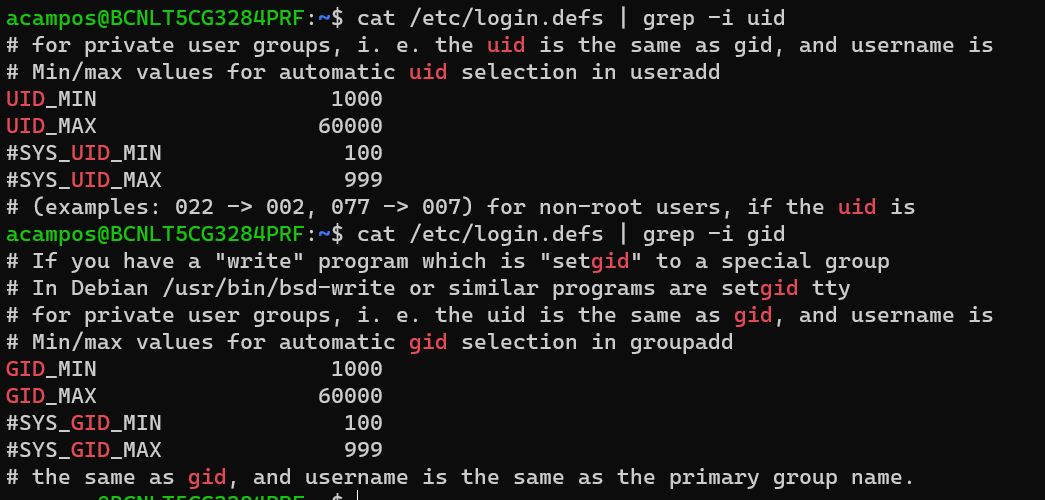
\includegraphics[scale=0.7]{pictures/defsbig.png}
    \centering
\end{figure}
\end{blocktemplateI}



So you can trim the output using AWK or cut:
\begin{codetemplate}{}
\begin{verbatim}
$ awk -F ":" '{ print $1 }' /etc/passwd
\end{verbatim}
\end{codetemplate}
\begin{codetemplate}{}
\begin{verbatim}
$ cut -d ":" -f1 /etc/passwd
\end{verbatim}
\end{codetemplate}

\begin{blocktemplate}{NOTE}
We will discuss passwords in the next sect, but expect to see an "x" in the password field of this file.
\end{blocktemplate}

\subsubsection{Understand the /etc/shadow file}
Long ago, password hashes were stored in the \verb|/etc/passwd| file. This file was world-readable, allowing inquisitive users to pull password hashes for other accounts from the file and run them through password-cracking utilities. Eventually, the password hashes were moved to a file readable only by root: \verb|/etc/shadow|. Today, the password field in the \verb|/etc/passwd| file is marked with an x.

\begin{blocktemplateI}{NOTE}
To know more about the passwords, the value we can see in the \verb|/etc/passwd| is a hashed value, produced by the crypt function in Linux when we set the passphrase for the user using the passwd command. The hashed passphrase follows a specific format:
\begin{codetemplate}{}
\begin{verbatim}
$id$salt$hashedpassword
\end{verbatim}
\end{codetemplate}
\begin{itemize}
    \item \textbf{id:} is the hashing method used when hashing the passphrase. For example, if the hash value is produced by yescrypt, the ID will be y, and 6 if the sha512crypt method is used. For a complete list of hashing methods and their ID, we can refer to the \href{https://manpages.debian.org/unstable/libcrypt-dev/crypt.5.en.html}{Official Documentation}.
    \item \textbf{salt:} adding random data to the input of a hash function to guarantee a unique output, the hash, even when the inputs are the same.
    \item \textbf{hashedpassword:} the password encrypted
\end{itemize}
\end{blocktemplateI}

\subsubsection{Add User to Linux System}
\paragraph{Basic Addition}
\begin{codetemplate}{}
\begin{verbatim}
$ sudo useradd [OPTIONS] user_name
\end{verbatim}
\end{codetemplate}
When invoked, \verb||useradd| creates a new user account according to the options specified on the command line and the default values set in the \verb|/etc/default/useradd| file.

\begin{blocktemplateII}{NOTE}
When executed without any option, useradd creates a new user account using the default settings specified in the /etc/default/useradd file.
\end{blocktemplateII}

\begin{blocktemplateIII}{WARNING}
Only root or users with sudo privileges can use the \verb|useradd| command to create new user accounts.
\end{blocktemplateIII}

\textbf{To check the user has been correctly created}
\begin{codetemplate}{}
\begin{verbatim}
$ id username
\end{verbatim}
\end{codetemplate}

\textbf{To be able to log in as the newly created user, you need to set the user password}
\begin{codetemplate}{}
\begin{verbatim}
$ sudo passwd username
\end{verbatim}
\end{codetemplate}
You will be prompted to enter and confirm the password. Make sure you use a strong password.

\paragraph{Addition with Home Directory Creation}
On most Linux distributions, when creating a new user account with useradd, \textbf{by default the user’s home directory is not created}.

\textbf{Use the} \verb|-m (--create-home)| \textbf{option to create the user home directory as} \verb|/home/username|
\begin{codetemplate}{}
\begin{verbatim}
$ sudo useradd -m username
\end{verbatim}
\end{codetemplate}
The command above creates the new user’s home directory and copies files from \verb|/etc/skel| directory to the user’s home directory. If you list the files in the /home/username directory, you will see the initialization files:
\begin{itemize}
    \item \verb|.bash_logout|
    \item \verb|.bashrc|
    \item \verb|.profile|
\end{itemize}

\begin{figure}[H]
    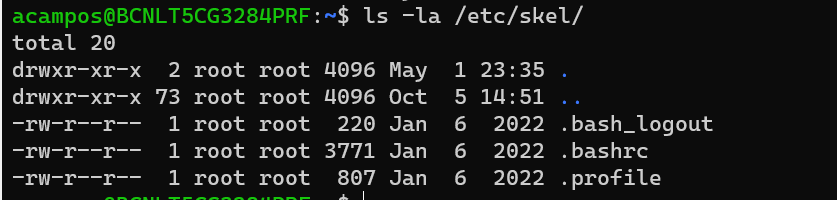
\includegraphics[scale=0.7]{pictures/etcskel.png}
    \centering
\end{figure}

\begin{blocktemplate}{NOTE}
Within the home directory, the user can write, edit and delete all files and directories.
\end{blocktemplate}

\textbf{To create another different home}
\begin{codetemplate}{}
\begin{verbatim}
$ sudo useradd -d /custom/home username
\end{verbatim}
\end{codetemplate}

\paragraph{Custom Shell}
\begin{codetemplate}{}
\begin{verbatim}
$ sudo useradd -s /custom/shell username
\end{verbatim}
\end{codetemplate}


\paragraph{Addition Specifing the UID}
By default, when a new user is created, the system assigns the next available UID from the range of user IDs specified in the \verb|/etc/login.defs| file.

\begin{figure}[H]
    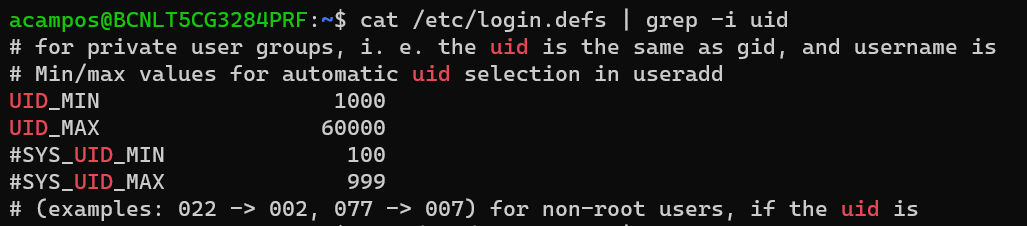
\includegraphics[scale=0.7]{pictures/loginsfile.png}
    \centering
\end{figure}

Invoke useradd with the -u (--uid) option to create a user with a specific UID. For example to create a new user named username with UID of 1500 you would type:
\begin{codetemplate}{}
\begin{verbatim}
$ sudo useradd -u 1500 username
\end{verbatim}
\end{codetemplate}

\begin{blocktemplateIII}{WARNING}
If the specified UID is already allocated to another user, you're alerted that the UID is unavailable and the operation aborts. Rerun it with a different UID number.
\end{blocktemplateIII}

\begin{blocktemplateI}{NOTE}
An easy way to look your user UID:
\begin{codetemplate}{}
\begin{verbatim}
$ id -u username
\end{verbatim}
\end{codetemplate}
\end{blocktemplateI}

\paragraph{Addition Specifing the GID}
When creating a new user, the default behavior of the useradd command is to create a group with the same name as the username, and same GID as UID.

The \verb|-g| (\verb|--gid|) option allows you to create a user with a specific initial login group. You can specify either the group name or the GID number. The group name or GID must already exist.
\begin{codetemplate}{}
\begin{verbatim}
$ sudo useradd -g group username
\end{verbatim}
\end{codetemplate}

\begin{blocktemplateIII}{WARNING}
If the specified group ID is already allocated to another group, you're alerted that the GID is unavailable and the operation aborts. Rerun it with a different group ID number.
\end{blocktemplateIII}

\begin{blocktemplateI}{NOTE}
An easy way to look your user primary group:
\begin{codetemplate}{}
\begin{verbatim}
$ id -gn username
\end{verbatim}
\end{codetemplate}
\end{blocktemplateI}

\paragraph{Addition Assigning Multiple Groups}

There are two types of groups in Linux operating systems Primary group and Secondary (or supplementary) group. Each user can belong to \textbf{exactly one primary} group and\textbf{ zero or more secondary groups}.

You to specify a list of supplementary groups which the user will be a member of with the \verb|-G| (\verb|--groups|) option.
\begin{codetemplate}{}
\begin{verbatim}
$ sudo useradd -g primary_group -G sec_group1, sec_group2, sec_group3 username
\end{verbatim}
\end{codetemplate}

\begin{blocktemplateI}{NOTE}
An easy way to look all your user configuration:
\begin{codetemplate}{}
\begin{verbatim}
$ id username
\end{verbatim}
\end{codetemplate}
\end{blocktemplateI}

\paragraph{Addition with more Configurations}
To create users with more different configurations, you can check the \href{https://linuxize.com/post/how-to-create-users-in-linux-using-the-useradd-command/}{documentation}.

\subsubsection{Switching User in Linux - su command}

Su allows you to change the existing user to some other user. Use the \verb|–l username| method to define a user account if you need to execute a command as someone other than root.

\subsubsection{Delete User in Linux System}
 Deleting a user requires deleting both the user account as well as the files that are connected with the user account. With this command you do both:
\begin{codetemplate}{}
\begin{verbatim}
$ userdel -r username
\end{verbatim}
\end{codetemplate}

\begin{blocktemplateIII}{WARNING}
The above command deletes the user whose username is provided. Make sure that the user is not part of a group. If the user is part of a group then it will not be deleted directly, hence we will have to first remove him from the group and then we can delete him.  
\end{blocktemplateIII}

\subsubsection{Manage User from Linux System}
\textbf{Change the home directory}
\begin{codetemplate}{}
\begin{verbatim}
$ usermod -d new_home_directory_path username
\end{verbatim}
\end{codetemplate}

\textbf{Change login name}
\begin{codetemplate}{}
\begin{verbatim}
$ sudo usermod -l new_login_name old_login_name
\end{verbatim}
\end{codetemplate}

\textbf{Change the user password}
\begin{codetemplate}{}
\begin{verbatim}
$ passwd
\end{verbatim}
\end{codetemplate}

\begin{blocktemplateIII}{WARNING}
It will require authentication with the old password, so you should know the old password to change it this way.

If you do not know the user password, you can use the sudo user to do it:
\textbf{Change the user password}
\begin{codetemplate}{}
\begin{verbatim}
$ sudo passwd username
\end{verbatim}
\end{codetemplate}
\end{blocktemplateIII}

\begin{blocktemplateI}{NOTE}
Even further, you can force Linux user to change password at their next login, check the \href{https://www.cyberciti.biz/faq/linux-set-change-password-how-to/}{documentation}
\end{blocktemplateI}

\textbf{Modify the UID of a user}
\begin{codetemplate}{}
\begin{verbatim}
$ usermod -u  new_uid username
\end{verbatim}
\end{codetemplate}

\textbf{Modify the group GID of a user}
\begin{codetemplate}{}
\begin{verbatim}
$ usermod -g  new_gid username
\end{verbatim}
\end{codetemplate}

\subsubsection{SSH Key-Based Authentication}
Secure Shell (SSH) key-based authentication provides a more secure alternative to password-based authentication. Users generate a public-private key pair, where the public key is stored on the server and the private key is kept securely on the user's device.

With SSH key-based authentication, users like Lisa, a system administrator at CTechCo, can authenticate without entering a password. Instead, the server verifies the user's identity based on the possession of the private key.

To configure SSH key-based authentication for Lisa, the following steps can be taken:

\begin{itemize}
    \item Generate an SSH key pair on Lisa's machine using the ssh-keygen command.
    \item Copy the public key to the server's \verb|/home/lisasmith/.ssh/authorized_keys| file.
    \item Configure the server to allow SSH key-based authentication.
\end{itemize}


\subsection{Managing Linux Groups}
In Linux, groups are collections of users. Creating and managing groups is one of the simplest ways to deal with multiple users simultaneously, especially when dealing with permissions. It's more efficient to group user accounts with similar access requirements than to manage permissions on a user-by-user basis.


\subsubsection{Understanding the /etc/group file}
Similar to the \verb|/etc/passwd| file above, the \verb|/etc/group| file contains group account information. This information can be essential for troubleshooting, security audits, and ensuring users can access the resources they need.

The fields in the \verb|/etc/group| file are:
\begin{codetemplate}{}
\begin{verbatim}
groupname:password:GID:group members
\end{verbatim}
\end{codetemplate}

\subsubsection{Add a Group in Linux}
To create a new group:
\begin{codetemplate}{}
\begin{verbatim}
$ sudo groupadd group_name
\end{verbatim}
\end{codetemplate}

To view the group you just added, run the command below:
\begin{codetemplate}{}
\begin{verbatim}
$ cat /etc/group | grep -i group_name
\end{verbatim}
\end{codetemplate}

\begin{blocktemplate}{NOTE}
When a group is created, a unique group ID gets assigned to that group. You can verify that the group appears (and see its group ID) by looking in the \verb|/etc/group| file.
\end{blocktemplate}

If you want to create a group with a specific group ID (GID), use the \verb|--gid| or \verb|-g| option:

\begin{codetemplate}{}
\begin{verbatim}
$ sudo groupadd -g 1009 group_name
\end{verbatim}
\end{codetemplate}

\begin{blocktemplateIII}{WARNING}
If the specified group ID is already allocated to another group, you're alerted that the GID is unavailable and the operation aborts. Rerun it with a different group ID number.
\end{blocktemplateIII}

\subsubsection{Change the group ID}
You can change the group ID of any group with the \verb|groupmod| command and the \verb|--gid| or \verb|-g| option:
\begin{codetemplate}{}
\begin{verbatim}
$ sudo groupmod -g 1011 demo1
\end{verbatim}
\end{codetemplate}

\subsubsection{Rename a group}
You can rename a group using \verb|groupmod| with the \verb|--new-name| or \verb|-n| option:
\begin{codetemplate}{}
\begin{verbatim}
$ sudo groupmod -n test demo1
\end{verbatim}
\end{codetemplate}

\subsubsection{How to Assign Users to Groups in Linux}

Once a group is created, users can be added to it in the following way:
\begin{codetemplate}{}
\begin{verbatim}
$ sudo usermod -aG group_name username
\end{verbatim}
\end{codetemplate}

To check the user has been successfully added:
\begin{codetemplate}{}
\begin{verbatim}
$ id username
\end{verbatim}
\end{codetemplate}

\subsubsection{How to Delete Users from Groups in Linux}
To remove a specific user from a group, you can use the gpasswd command to modify group information:
\begin{codetemplate}{}
\begin{verbatim}
$ sudo gpasswd --delete username group_name
\end{verbatim}
\end{codetemplate}

\subsubsection{How to delete a group}
When a group is no longer needed, you delete it by using the groupdel command:

\begin{codetemplate}{}
\begin{verbatim}
$ sudo groupdel demo
\end{verbatim}
\end{codetemplate}

\subsection{Sudo Command}
The sudo command allows you to run programs as the root user. Using sudo instead of login in as root is more secure because you can grant limited administrative privileges to individual users without them knowing the root password. \textbf{That's why the root user account in Ubuntu is disabled by default for security reasons, and users are encouraged to perform system administrative tasks using sudo}. The initial user created by the Ubuntu installer is already a member of the sudo group, so if you are running Ubuntu, chances are that the user you are logged in as is already granted with sudo privileges.

\subsubsection{Give sudo permissions with password}
By default, on most Linux distributions granting sudo access is as simple as adding the user to the sudo group defined in the sudoers file . Members of this group will be able to run any command as root. The name of the \textbf{group} may differ from distribution to distribution.

\begin{itemize}
    \item \verb|sudo:| Debian, Ubuntu and derivates groups for sudo permissions.
\begin{codetemplate}{}
\begin{verbatim}
$ usermod -aG sudo username
\end{verbatim}
\end{codetemplate}
    \item \verb|wheel:| RedHat, CentOs and Fedora group for sudo permissions
\begin{codetemplate}{}
\begin{verbatim}
$ usermod -aG wheel username
\end{verbatim}
\end{codetemplate}
\end{itemize}

We can see the permission groups allowed in the \verb|/etc/sudoers| file:

\begin{codetemplate}{}
\begin{verbatim}
$ sudo cat /etc/sudoers
\end{verbatim}
\end{codetemplate}

\begin{figure}[H]
    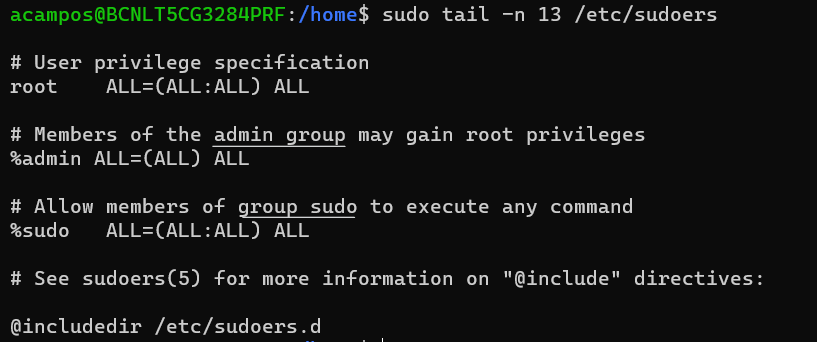
\includegraphics[width=\textwidth]{pictures/sudoers.png}
    \centering
\end{figure}

So in my Linux System, any user added to the groups \textbf{sudo} or \textbf{admin} will have all sudo permissions enabled.

\textbf{What would happen with a user that is not in these groups?}
\begin{figure}[H]
    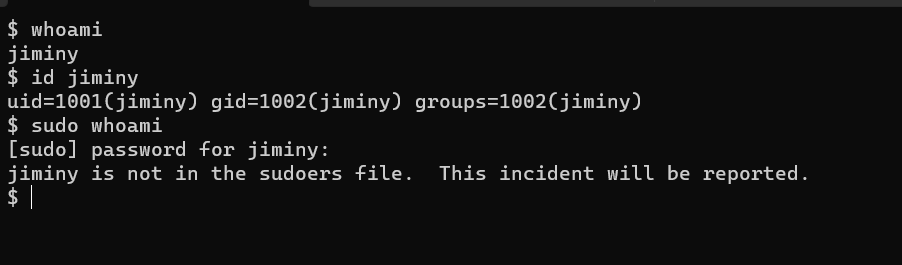
\includegraphics[width=\textwidth]{pictures/jiminy.png}
    \centering
\end{figure}

But if we add him to the admin group... Voilà!
\begin{figure}[H]
    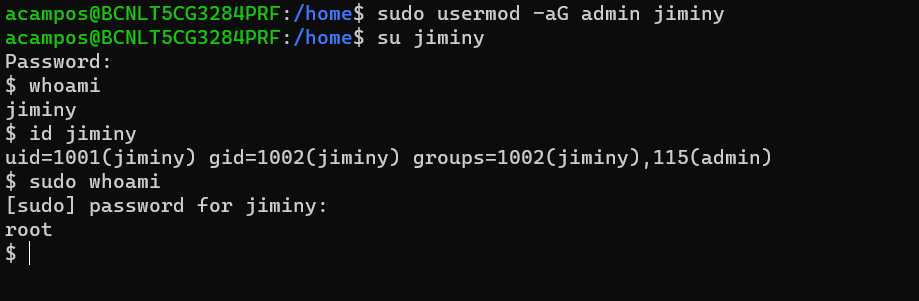
\includegraphics[width=\textwidth]{pictures/voliajiminy.png}
    \centering
\end{figure}

\begin{blocktemplateII}{NOTE}
The password you have to introduce to access to sudo permissions is the user password, in this case, the jiminy password.
\end{blocktemplateII}


\subsubsection{Give only some actions sudo permission}
To allow a specific user to run only certain programs as sudo, instead of adding the user to the sudo group, add the users to the \verb|/ect/sudoers| file. For example, to allow the user linuxize to run only the mkdir command:

\begin{blocktemplateIII}{WARNING}
Modifying \verb|/etc/sudoers| file can be very dangerous, so do it carefully. \textbf{Se puede liar muy parda!}
\\\\
Advices:
\begin{itemize}
    \item Use \textbf{sudo visudo}, because visudo will warn you that there’s a syntax error and asks to undo the changes.
    \item It is hardly recommended to make a copy of the file before
\begin{codetemplate}{}
\begin{verbatim}
$ sudo cp /etc/sudoers sudoerscopy
\end{verbatim}
\end{codetemplate}
\end{itemize}
\end{blocktemplateIII}
Just if you  know what you're doing, keep going:
\begin{codetemplate}{}
\begin{verbatim}
$ sudo visudo
\end{verbatim}
\end{codetemplate}

\begin{codetemplate}{/etc/sudoers}
\begin{verbatim}
linuxize  ALL=/bin/mkdir
\end{verbatim}
\end{codetemplate}

\begin{blocktemplate}{NOTE}
The file you are oppening with \verb|sudo visudo| is the \verb|/etc/sudoers| file with the Nano editor! If you are not used to Nano, you can open it with vim. But vim does not notify you if there are some syntax error in the file, nano does.
\begin{codetemplate}{}
\begin{verbatim}
$ sudo vim /etc/sudoers
\end{verbatim}
\end{codetemplate}
\end{blocktemplate}

\subsubsection{How to enable sudo without entering a password}
Modifying the \verb|/etc/sudoers| adding the user with the following:

\begin{blocktemplateIII}{WARNING}
Modifying \verb|/etc/sudoers| file can be very dangerous, so do it carefully. \textbf{Se puede liar muy parda!}
\\\\
Advices:
\begin{itemize}
    \item Use \textbf{sudo visudo}, because visudo will warn you that there’s a syntax error and asks to undo the changes.
    \item It is hardly recommended to make a copy of the file before
\begin{codetemplate}{}
\begin{verbatim}
$ sudo cp /etc/sudoers sudoerscopy
\end{verbatim}
\end{codetemplate}
\end{itemize}
\end{blocktemplateIII}

\begin{codetemplate}{}
\begin{verbatim}
$ sudo visudo
\end{verbatim}
\end{codetemplate}
\begin{codetemplate}{/etc/sudoers}
\begin{verbatim}
jiminy ALL=(ALL:ALL) NOPASSWD: ALL
\end{verbatim}
\end{codetemplate}

\begin{figure}[H]
    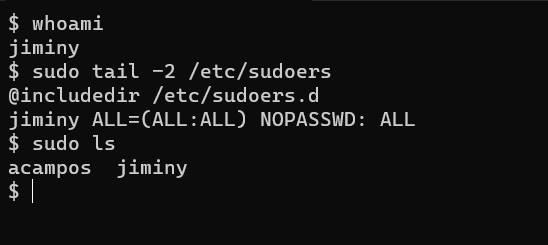
\includegraphics[scale=0.8]{pictures/jiminyboss.png}
    \centering
\end{figure}

Also you can modify it in the group configuration:
\begin{codetemplate}{/etc/sudoers}
\begin{verbatim}
# Members of the admin group may gain root privileges without pwd
%admin  ALL=(ALL) NOPASSWD: ALL
\end{verbatim}
\end{codetemplate}

\subsubsection{How to gain su permissions with sudo}
If you try to redirect the output of a command to a file that your user has no write permissions, you will get a “Permission denied" error.
\begin{codetemplate}{}
\begin{verbatim}
$ sudo echo "test" > /root/file.txt
# Output: bash: /root/file.txt: Permission denied
\end{verbatim}
\end{codetemplate}

This happens because the redirection \verb|“>"| of the output is performed under the user you are logged in, not the user specified with sudo. The redirection happens before the sudo command is invoked.

One solution is to invoke a new shell as root by using \verb|sudo sh -c|:

\begin{codetemplate}{}
\begin{verbatim}
$ sudo sh -c 'echo "test" > /root/file.txt'
\end{verbatim}
\end{codetemplate}

Another option is to pipe the output as a regular user to the tee command , as shown below:

\begin{codetemplate}{}
\begin{verbatim}
$ sudo echo "test" | sudo tee /root/file.txt
\end{verbatim}
\end{codetemplate}

\subsection{Su - root user}

As we comment in the previous section, Using sudo instead of login in as root is more secure because you can grant limited administrative privileges to individual users without them knowing the root password. \textbf{That's why the root user account in Ubuntu is disabled by default for security reasons, and users are encouraged to perform system administrative tasks using sudo}.

\subsubsection{First Approach - Enabling root account temporary}
If you only need the root account for a particular task or job, run the following command and supply the super user password to authenticate the action with sudo.
\begin{codetemplate}{}
\begin{verbatim}
$ sudo –i
\end{verbatim}
\end{codetemplate}

What behind the scenes this command makes is to enable the root user only in the current shell (associated Linux process), and when this shell is shot down (for example typing exit) and you come back to you user, the root will be disabled again.

\subsubsection{Enable root user}
\begin{codetemplate}{}
\begin{verbatim}
$ sudo –i passwd root
\end{verbatim}
\end{codetemplate}

You will have to enter the new password for the root user and go ahead.

\begin{figure}[H]
    
\includegraphics[scale=0.8]{pictures/su.png}
    \centering
\end{figure}

\subsubsection{Disable root user}
\begin{codetemplate}{}
\begin{verbatim}
$ sudo passwd -dl root
\end{verbatim}
\end{codetemplate}

\begin{figure}[H]
    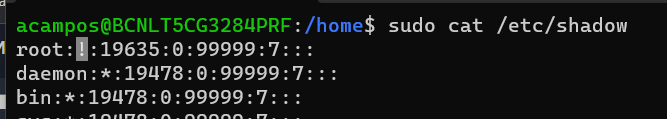
\includegraphics[scale=0.7]{pictures/nopwdsu.png}
    \centering
\end{figure}

\newpage
%-------------------------------------------------------------------------------------------------
\section{Basic Linux Commands}

\subsection{Linux System Information}
\textbf{Prints information about your machine’s kernel, name, and hardware}
\\ \textbf{The order is: }kernel name, network node hostname, kernel release, kernel version, machine hardware name, processor type, hardware platform and os.
\begin{codetemplate}{}
\begin{verbatim}
$ uname -a
\end{verbatim}
\end{codetemplate}

\textbf{To check Linux Distro}
\begin{codetemplate}{}
\begin{verbatim}
$ uname -or
\end{verbatim}
\end{codetemplate}

\textbf{To know more about Linux Distro}
\begin{codetemplate}{}
\begin{verbatim}
$ cat /etc/os-release
\end{verbatim}
\end{codetemplate}
\begin{codetemplate}{}
\begin{verbatim}
$ cat /etc/lsb-release
\end{verbatim}
\end{codetemplate}
\begin{codetemplate}{}
\begin{verbatim}
$ lsb_release -a
\end{verbatim}
\end{codetemplate}
\begin{codetemplate}{}
\begin{verbatim}
$ hostnamectl
\end{verbatim}
\end{codetemplate}

\subsection{Linux System Consumption}
\textbf{Displays running processes and the system’s resource usage}
\begin{codetemplate}{}
\begin{verbatim}
$ top
\end{verbatim}
\end{codetemplate}

Do the same but with some colorfull graphics
\begin{codetemplate}{}
\begin{verbatim}
$ htop
\end{verbatim}
\end{codetemplate}

\textbf{Displays the system’s overall disk space usage}
\begin{codetemplate}{}
\begin{verbatim}
$ df -h
\end{verbatim}
\end{codetemplate}

\textbf{Displays a folder/file disk space usage}
\begin{codetemplate}{}
\begin{verbatim}
$ df -h folder_name
\end{verbatim}
\end{codetemplate}

\textbf{Checks a file or directory’s storage consumption}
\begin{codetemplate}{}
\begin{verbatim}
$ du -h directory_name
\end{verbatim}
\end{codetemplate}

\begin{blocktemplate}{NOTE}
\verb|-h| flag shows an humanize output, it specifies K, M, G, etc. If you want to have the output in Kibibyte do not use the flag.
\end{blocktemplate}

\subsection{Linux Services}

\subsubsection{ps}
ps displays information about a selection of the active processes.  If you want a repetitive update of the selection and the displayed information, use top instead.
\textbf{Display a snapshot of the currently running processes}
\begin{codetemplate}{}
\begin{verbatim}
$ ps waux
\end{verbatim}
\end{codetemplate}
\begin{itemize}
    \item \textbf{w:} display the full command line of each process
    \item \textbf{a:} list processes from all users
    \item \textbf{u:} detailed information about each process
    \item \textbf{x:} list processes without controlling terminals
\end{itemize}

\subsubsection{systemctl}
\textbf{Systemctl} manages systemd services and other units such as sockets, devices, mount points, and timers in Linux systems. It is a powerful command-line tool used to query or send control commands to the system manager.

\textbf{Systemd} is a system and service manager for Linux operating systems

\textbf{Start a Service}
\begin{codetemplate}{}
\begin{verbatim}
$ systemctl start <service_name>
\end{verbatim}
\end{codetemplate}

\textbf{Stop a Service}
\begin{codetemplate}{}
\begin{verbatim}
$ systemctl stop <service_name>
\end{verbatim}
\end{codetemplate}

\textbf{Check the status of a Service}
\begin{codetemplate}{}
\begin{verbatim}
$ systemctl status <service_name>
\end{verbatim}
\end{codetemplate}

\textbf{Restart a Service:} if the service is very critical, check \verb|systemctl reload|
\begin{codetemplate}{}
\begin{verbatim}
$ systemctl restart <service_name>
\end{verbatim}
\end{codetemplate}

\textbf{Reload configuration of a Service:} very useful for critical services that cannot be restarted, it is like a soft restart.
\begin{codetemplate}{}
\begin{verbatim}
$ systemctl reload <service_name>
\end{verbatim}
\end{codetemplate}

\textbf{Enable a service to start on Boot}
\begin{codetemplate}{}
\begin{verbatim}
$ systemctl enable <service_name>
\end{verbatim}
\end{codetemplate}

\textbf{Disable a service to start on Boot}
\begin{codetemplate}{}
\begin{verbatim}
$ systemctl disable <service_name>
\end{verbatim}
\end{codetemplate}

\textbf{Show the running services}
\begin{codetemplate}{}
\begin{verbatim}
$ systemctl --type=service --state=running
\end{verbatim}
\end{codetemplate}

\subsection{Service}

The \textbf{service} command is commonly used in older versions of Linux distributions or those that haven't fully adopted systemd yet. It provides a simpler interface compared to systemctl, but it offers similar functionality for starting, stopping, restarting, and checking the status of services.

It is very similar to \textbf{systemctl}, with almost same functionalities, just reversing arguments

\textbf{Start a Service}
\begin{codetemplate}{}
\begin{verbatim}
$ service <service_name> start
\end{verbatim}
\end{codetemplate}

\textbf{Check the status of a Service}
\begin{codetemplate}{}
\begin{verbatim}
$ service <service_name> status
\end{verbatim}
\end{codetemplate}

\subsection{Journalctl}
journalctl and systemctl are command-line utilities in Linux systems that are commonly used for managing and monitoring system services and logs. They are part of the systemd suite of tools, which is a system and service manager for Linux operating systems.

\textbf{journalctl} is a command-line tool used to query and display logs from the systemd journal. The systemd journal is a component of systemd that collects and stores log messages from the kernel, services, and other system components in a structured binary format.
journalctl allows you to view and filter logs collected by the systemd journal. This includes logs from various services, system messages, kernel logs, and more.

\subsubsection{Usage}

Display all available logs:
\begin{codetemplate}{}
\begin{verbatim}
$ journalctl
\end{verbatim}
\end{codetemplate}

Display logs from current boot:
\begin{codetemplate}{}
\begin{verbatim}
$ journalctl -b 
\end{verbatim}
\end{codetemplate}

Display logs from previous boot:
\begin{codetemplate}{}
\begin{verbatim}
$ journalctl -b -1
\end{verbatim}
\end{codetemplate}

Display logs associated to a specific service:
\begin{codetemplate}{}
\begin{verbatim}
$ journalctl -u <service_name>
\end{verbatim}
\end{codetemplate}

Display latest logs:
\begin{codetemplate}{}
\begin{verbatim}
$ journalctl -e
\end{verbatim}
\end{codetemplate}

Detailed logs:
\begin{codetemplate}{}
\begin{verbatim}
$ journalctl -x
\end{verbatim}
\end{codetemplate}

Follow the logs in real time:
\begin{codetemplate}{}
\begin{verbatim}
$ journalctl -f
\end{verbatim}
\end{codetemplate}

Show logs since:
\begin{codetemplate}{}
\begin{verbatim}
$ journalctl --since "YYYY-MM-DD HH:MM:SS"
\end{verbatim}
\end{codetemplate}

Show logs until:
\begin{codetemplate}{}
\begin{verbatim}
$ journalctl --until "YYYY-MM-DD HH:MM:SS"
\end{verbatim}
\end{codetemplate}

Filter logs based on priority
\begin{codetemplate}{}
\begin{verbatim}
$ journalctl -p <priority>
\end{verbatim}
\end{codetemplate}
\begin{codetemplate}{}
\begin{verbatim}
$ journalctl -p err
\end{verbatim}
\end{codetemplate}

\begin{blocktemplate}{Note}
Most used:
\begin{codetemplate}{}
\begin{verbatim}
$ journalctl -xeu <service_name>
\end{verbatim}
\end{codetemplate}

But remember that most relevant logs \textbf{are in the specific log file of the service}.
\end{blocktemplate}

\subsection{Moving between directories}
\subsubsection{Introduction}
\begin{itemize}
    \item \verb+pwd:+ which directory we are
    \item \verb+cd == cd ~ :+ go to users \verb+$HOME+
    \item \verb+cd /+ : go to /
    \item \verb+cd .+ : does not do anything
    \item \verb+cd ..+ : go one directory back
    \item \verb+ls -l+ : list all directory content (not hidden)
    \item \verb+ls -la+ : list all directory content (hidden or not)
\end{itemize}

\subsubsection{ls -la Analyzing Results}
The first character on the left represents the type, possible values for this position are as follows:

\begin{itemize}
    \item \textbf{-:} file
    \item \textbf{d:} directory
    \item \textbf{l:} symbolic link
    \item \textbf{b:} binary (executable file)
\end{itemize}

The following 9 represent the file permissions and should be viewed in groups of 3.

\begin{itemize}
    \item Los \textbf{first 3} owner permissions 
    \item Los \textbf{3 in the middle} group permissions
    \item Los \textbf{last 3} rest of the world permissions
\end{itemize}
\begin{itemize}
    \item \textbf{r:} read
    \item \textbf{w:} write 
    \item \textbf{x:} execute
\end{itemize}

\begin{blocktemplateII}{Note}
The \verb+/etc/group+ is a text file which defines the groups to which users belong under Linux and UNIX operating system. Under Unix / Linux multiple users can be categorized into groups. Unix file system permissions are organized into three classes, user, group, and others. The use of groups allows additional abilities to be delegated in an organized fashion, such as access to disks, printers, and other peripherals    
\end{blocktemplateII}

\subsection{chmod}

You may need to know how to change permissions in numeric code in Linux, so to do this you use numbers instead of “r", “w", or “x". Cause Basically, you add up the numbers depending on the level of permission you want to give.

\begin{itemize}
    \item \textbf{0:} No Permission
    \item \textbf{1:} Execute
    \item \textbf{2:} Write
    \item \textbf{4:} Read
\end{itemize}

\underline{Examples:}

\begin{itemize}
    \item To give read, write, and execute permissions for everyone:
\begin{codetemplate}{}
\begin{verbatim}
$ chmod 777 folder/file_name
\end{verbatim}
\end{codetemplate}

    \item To give read, write, and execute permissions for the owner user only.
\begin{codetemplate}{}
\begin{verbatim}
$ chmod 700 folder/file_name
\end{verbatim}
\end{codetemplate}

    \item To give write and execute (3) permission for the owner user, w (2) for the group, and read, write, and execute for the rest of users.
\begin{codetemplate}{}
\begin{verbatim}
$ chmod 321 foldername
\end{verbatim}
\end{codetemplate}
\end{itemize}

\begin{figure}[H]
    \centering
    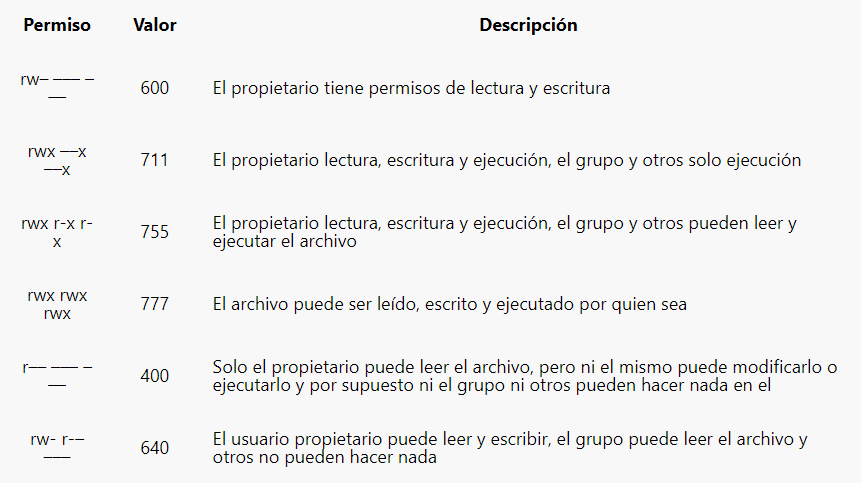
\includegraphics[scale=0.55]{pictures/chmod.PNG}
    \caption{Permissions}
    \label{chmod}
\end{figure}

\subsection{chown}
The \verb|chown| command allows you to change the user and/or group ownership of a given file, directory, or symbolic link.

In Linux, all files are associated with an owner and a group and assigned with permission access rights for the file owner, the group members, and others.

\begin{codetemplate}{}
\begin{verbatim}
$ chown [OPTIONS] USER[:GROUP] FILE(s)
\end{verbatim}
\end{codetemplate}

\textbf{USER} is the user name or the user ID (UID) of the new owner. \textbf{GROUP} is the name of the new group or the group ID (GID). FILE(s) is the name of one or more files, directories or links.

\begin{blocktemplate}{NOTE}
Numeric IDs should be prefixed with the + symbol.
\end{blocktemplate}

For example, the following command will change the ownership of a file named file1 to a new owner named \verb|linuxize|:
\begin{codetemplate}{}
\begin{verbatim}
$ chown linuxize file1
\end{verbatim}
\end{codetemplate}

\textbf{To change recursively}
\begin{codetemplate}{}
\begin{verbatim}
$ chown -R linuxize /var/www/
\end{verbatim}
\end{codetemplate}

\begin{blocktemplateII}{NOTE}
If the directory contains symbolic links you should add the flag \verb|-h|
\begin{codetemplate}{}
\begin{verbatim}
$ chown -hR linuxize /var/www/
\end{verbatim}
\end{codetemplate}
\end{blocktemplateII}

\textbf{Using a Reference File}
The \verb|--reference=ref_file| option allows you to change the user and group ownership of given files to be same as those of the specified reference file (\verb|ref_file|). 
\begin{codetemplate}{}
\begin{verbatim}
$ chown --reference=REF_FILE FILE
\end{verbatim}
\end{codetemplate}

\begin{blocktemplateIII}{WARNING}
If the reference file is a symbolic link chown will use the user and group of the target file.
\end{blocktemplateIII}

\subsection{Ctrl+R}

With this command we can search in the history the past commands we have run on the machine.

Be carefull using Ctrl+R, because for example if you click on tab, you will crash it:

\begin{itemize}
    \item \textbf{Intro:} to execute the command it is showing you
    \item \textbf{Ctrl+R:} to go to the command behind that matches the pattern
\end{itemize}

\subsection{Mkdir (create files)}
\begin{itemize}
    \item \verb+mkdir -p+: create a directory recursively, with different subfolders (mkdir -p first/second/third…)
    \item \verb+mkdir -m a=rwx+: create a directory which files are going to have the permissions specified
    \item \verb+rm -rf <file>+: remove recursively the file
    \item \verb+rm *.txt+: remove all the files which contains the string "txt" on the current directory
\end{itemize}

\subsection{Mv}
Rename SOURCE to DEST, or move SOURCE(s) to DIRECTORY.
\begin{codetemplate}{}
\begin{verbatim}
$ mv path/to/source path/to/dest
\end{verbatim}
\end{codetemplate}

\begin{itemize}
    \item \textbf{-t:} Moving different files to DEST
\begin{codetemplate}{}
\begin{verbatim}
$ mv -t path/to/dest path/to/source_1 path/to/source_2 ... path/to/source_n
\end{verbatim}
\end{codetemplate}

    \item \verb|-i:| prompts the user before overwriting an existing file.
    \item \verb|-f:| forces the move operation without prompting for confirmation, even if it means overwriting files.
    \item \verb|-n:| prevents overwritting existing files.
    \item \verb|-v:| verbose.
    \item \textbf{Move content from one folder to another}
\begin{codetemplate}{}
\begin{verbatim}
$ mv path/to/source/* /path/dest/folder/
\end{verbatim}
\end{codetemplate}
\end{itemize}

\subsection{Cp}
Copy SOURCE to DEST, or multiple SOURCE(s) to DIRECTORY.

\begin{codetemplate}{}
\begin{verbatim}
$ cp path/to/source path/to/dest
\end{verbatim}
\end{codetemplate}

\begin{itemize}
    \item \verb|-r / -R / --recursively:| Recursively.
\begin{codetemplate}{}
\begin{verbatim}
$ cp -r path/to/source path/to/dest
\end{verbatim}
\end{codetemplate}

    \item \verb|-t:| Copying different files to DEST.
\begin{codetemplate}{}
\begin{verbatim}
$ cp -t path/to/dest path/to/source_1 path/to/source_2 ... path/to/source_n
\end{verbatim}
\end{codetemplate}

    \item \verb|-p:| preserves the original file's attributes, such as the timestamp, ownership, and permissions.
    \item \verb|-f:| forces the copy operation without prompting for confirmation, even if it means overwriting files.
    \item \verb|-n:| prevents overwritting existing files.
    \item \verb|-v:| verbose.
    \item \textbf{Copy all the content from one folder to another:}
\begin{codetemplate}{}
\begin{verbatim}
$ cp -r path/to/source/* /path/dest/folder/
\end{verbatim}
\end{codetemplate}
\end{itemize}

\subsection{Rsync}
Rsync is a fast and extraordinarily versatile file copying tool.  It can copy locally,  to/from  another  host over any remote shell, or to/from a remote rsync daemon.  
It offers a large number of options that control every aspect of its behavior and permit very flexible specification of the set of files to be copied.  
It is famous  for its delta-transfer algorithm, which reduces the amount of data sent over the network by sending only the differences between the source files and the existing files in the destination.  
Rsync is widely used  for backups and mirroring and as an improved copy command for everyday use.
\begin{codetemplate}{}
\begin{verbatim}
$ rsync -av /path/to/source/ /path/to/destination/
\end{verbatim}
\end{codetemplate}

\begin{itemize}
    \item \verb|-a:| enables archive mode, which preserves symbolic links, file permissions, user and group ownerships, and timestamps.
    \item \verb|-v:| verbose.
    \item \verb|-P:| displays the progress of the transfer, including the percentage of the transfer completed, transfer speed, and estimated time remaining. Also keep partially transferred files if the transfer is interrupted.
    \item \verb|--partial:| keep partially transferred files if the transfer is interrupted.
    \item \verb|--progress:| displays the progress of the transfer, including the percentage of the transfer completed, transfer speed, and estimated time remaining.
    \item \verb|--delete:| deletes files in the destination directory that are not present in the source directory. This keeps the destination directory in exact sync with the source.
    \item \textbf{From localhost to remote host:} 
\begin{codetemplate}{}
\begin{verbatim}
$ rsync -avzP /path/to/local/source \
    remote_user@remote_ip:/path/to/remote/destination
\end{verbatim}
\end{codetemplate}

    \item \textbf{From remote host to localhost:} 
\begin{codetemplate}{}
\begin{verbatim}
$ rsync -avzP remote_user@remote_ip:/path/to/remote/source \
    /path/to/local/destination 
\end{verbatim}
\end{codetemplate}
\end{itemize}

\begin{blocktemplateII}{Note}
You can specify the key to use: \verb|-e "ssh -i /path/to/private_key"|
\end{blocktemplateII}
    

\subsection{Simbolik Links}
\subsubsection{What is a Symbolic Link?}
A symbolic link (also known as a symlink or soft link) is a type of file that points to another file or directory in the Linux filesystem. Unlike hard links, which reference the data on the disk directly, a symbolic link contains a path that points to the target file or directory.

\subsubsection{Why Use Symbolic Links?}
Convenience: They allow you to create shortcuts to files and directories.
Flexibility: If the target file is moved, you can update the symlink without modifying the files that use it.
Resource Efficiency: They can link to directories and files across different filesystems.

\subsubsection{Symbolic Links Management}
The \verb|ln| command is used to create links between files. The \verb|-s| option creates a symbolic link. The basic syntax is:
\begin{codetemplate}{}
\begin{verbatim}
$ ln -s [target] [link_name]
\end{verbatim}
\end{codetemplate}

The unlink command is used to remove symbolic links. It only works with single files, not directories.
\begin{codetemplate}{}
\begin{verbatim}
$ unlink [link_name]
\end{verbatim}
\end{codetemplate}

\begin{blocktemplateI}{Note}
Alternatively, you can use the \verb|rm| command to remove symbolic links. This can be used for both files and directories.
\begin{codetemplate}{}
\begin{verbatim}
$ rm -rf [link_name]
\end{verbatim}
\end{codetemplate}
\end{blocktemplateI}

\subsection{Aliases}
To know all the aliases we have in our system
\begin{codetemplate}
\begin{verbatim}
$ alias
\end{verbatim}
\end{codetemplate}

\begin{figure}[H]
    \centering
    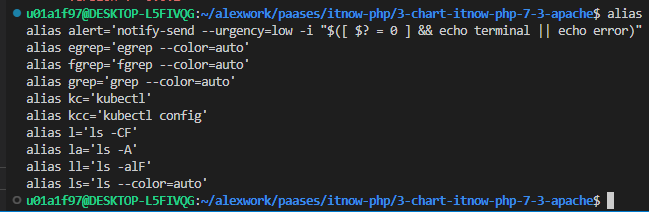
\includegraphics[scale=0.6]{pictures/image45.PNG}
    \caption{Default aliases}
\end{figure}

\subsubsection{Ephimeral Aliases}
To generate an ephimeral alias:
\begin{codetemplate}
\begin{verbatim}
$ alias <alias_name>="command arg1 arg2 ..."
\end{verbatim}
\end{codetemplate}
\underline{Examples}
\begin{codetemplate}
\begin{verbatim}
$ alias docker=podman
\end{verbatim}
\end{codetemplate}

\begin{codetemplate}
\begin{verbatim}
$ alias kcc="kubectl config"
\end{verbatim}
\end{codetemplate}

\subsubsection{Permanent Aliases}
To mantain alias in our system and do not lose them when we change of terminal we need to configure them on the shell config file we use:

\begin{itemize}
    \item Bash → \verb|~/.bashrc|
    \item ZSH → \verb|~/.zshrc|
    \item Fish → \verb|~/.config/fish/config.fish|
\end{itemize}

\begin{figure}[H]
    \centering
    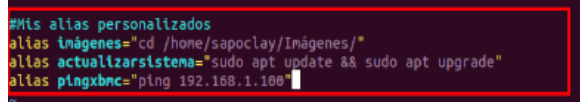
\includegraphics[scale=0.6]{pictures/image2.PNG}
    \caption{Alias in permanent files}
    \label{export}
\end{figure}

\subsection{Source}
\begin{codetemplate}
\begin{verbatim}
$ source filename [arguments]
\end{verbatim}
\end{codetemplate}

When you execute a command or a script from a shell, a subprocess (child process) of the shell is created to execute the command or script (parent process).

If the script that executes the child process creates or modifies any environment variable, those changes or variables disappear when the command or script finishes.

If we want those changes to remain, we can use the Bash command source. This command causes the process or command to execute without creating any child process, so that changes made to environment variables and others are maintained when the file finishes.

More information: \url{Source in Bash}

\subsection{Shutdown machines or terminals}
\begin{itemize}
    \item Shutdown the linux machine now
\begin{codetemplate}{}
\begin{verbatim}
$ sudo shutdown -r now
\end{verbatim}
\end{codetemplate}

    \item Just shutdown the terminal
\begin{codetemplate}{}
\begin{verbatim}
$ exec "$SHELL"
\end{verbatim}
\end{codetemplate}
\end{itemize}

\subsection{Others}
\textbf{To create a new empty file}
\begin{codetemplate}{}
\begin{verbatim}
$ touch main.py
\end{verbatim}
\end{codetemplate}

\textbf{Checks a file's type}
\begin{codetemplate}{}
\begin{verbatim}
$ file main.py
\end{verbatim}
\end{codetemplate}

\textbf{Prints command outputs in Terminal and a file}
\begin{codetemplate}{}
\begin{verbatim}
$ echo "Hello" | tee output.txt
\end{verbatim}
\end{codetemplate}

\href{https://www.hostinger.com/tutorials/linux-commands}{More basic interesting linux commands}

\newpage
%-------------------------------------------------------------------------------------------------
\section{Package Management Systems}

Package management systems in Linux handles the installation, updating, configuration, and removal of software packages. Each distribution has its own package management system, but they generally follow similar principles.

Key components of all package management systems:

\begin{itemize}
    \item \textbf{Repositories:} Central locations where software packages are stored and maintained
    \item \textbf{Packages:} Precompiled binaries or source code bundled with metadata, dependencies, and scripts necessary for installation.
    \item \textbf{Package Managers:} Tools that automate the process of handling packages.
\end{itemize}

\subsection{Apt - Debian}

Apt (Advanced Package Tool) package management system is built on top of the dpkg system, which is the underlying package management system for Debian-based distributions. It uses \textbf{APT Repositories}, servers that store software packages and provide metadata about those packages. Ubuntu repositories are organized into different sections like main, universe, restricted, and multiverse.

\subsubsection{Basic apt commands}

Update the local package index with the latest changes in the repositories:
\begin{codetemplate}
\begin{verbatim}
$ apt-get update
\end{verbatim}
\end{codetemplate}

Upgrades all installed packages to the latest versions available in the repositories:
\begin{codetemplate}
\begin{verbatim}
$ apt-get upgrade
\end{verbatim}
\end{codetemplate}

Simulates the upgrade:
\begin{codetemplate}
\begin{verbatim}
$ apt-get upgrade --dry-run
\end{verbatim}
\end{codetemplate}

Upgrade just a specific package:
\begin{codetemplate}
\begin{verbatim}
$ apt install --only-upgrade <package-name>
\end{verbatim}
\end{codetemplate}

Install the latest available version of a package:
\begin{codetemplate}
\begin{verbatim}
$ apt-get install <package_name>
\end{verbatim}
\end{codetemplate}

Install a specific version of a package:
\begin{codetemplate}
\begin{verbatim}
$ apt-get install <package_name>=<version>
\end{verbatim}
\end{codetemplate}
\begin{codetemplate}
\begin{verbatim}
$ apt-get install vim=2:8.1.2269-1ubuntu5
\end{verbatim}
\end{codetemplate}

List all installed packages and their versions on the system:
\begin{codetemplate}
\begin{verbatim}
$ apt-get list --installed
\end{verbatim}
\end{codetemplate}

Look for specific package installed and its version:
\begin{codetemplate}
\begin{verbatim}
$ apt-get list --installed | grep <package_name>
\end{verbatim}
\end{codetemplate}

Remove and purge package:
\begin{codetemplate}
\begin{verbatim}
$ apt-get remove <package_name>
\end{verbatim}
\end{codetemplate}
\begin{codetemplate}
\begin{verbatim}
$ apt-get purge <package_name>
\end{verbatim}
\end{codetemplate}

Remove unnecessary packages:
\begin{codetemplate}
\begin{verbatim}
$ apt-get clean
\end{verbatim}
\end{codetemplate}
\begin{codetemplate}
\begin{verbatim}
$ apt-get autoremove
\end{verbatim}
\end{codetemplate}

Look for the available versions of a package:
\begin{codetemplate}
\begin{verbatim}
$ apt-get update
\end{verbatim}
\end{codetemplate}
\begin{codetemplate}
\begin{verbatim}
$ apt-cache madison <package_name>
\end{verbatim}
\end{codetemplate}

Search for packages that match the provided keyword:
\begin{codetemplate}
\begin{verbatim}
$ apt-cache search <package_name>
\end{verbatim}
\end{codetemplate}

Show package details:
\begin{codetemplate}
\begin{verbatim}
$ apt-cache show <package_name>
\end{verbatim}
\end{codetemplate}

Check for broken dependencies:
\begin{codetemplate}
\begin{verbatim}
$ apt-get check
\end{verbatim}
\end{codetemplate}

\subsubsection{Managing Repositories}

The operating system creates two files to manage repositories:

\begin{itemize}
    \item \verb|/etc/apt/sources.list|: main configuration file for APT repositories. It contains a list of repository URLs where APT can find packages and updates. Mainly it includes official Ubuntu repositories that match your Ubuntu version and security repositories.
    \item \verb|/etc/apt/sources.list.d/:| repository updated by some packages when installed or updated to ensure their software is updated from their repositories. 
\end{itemize}

\begin{figure}[H]
    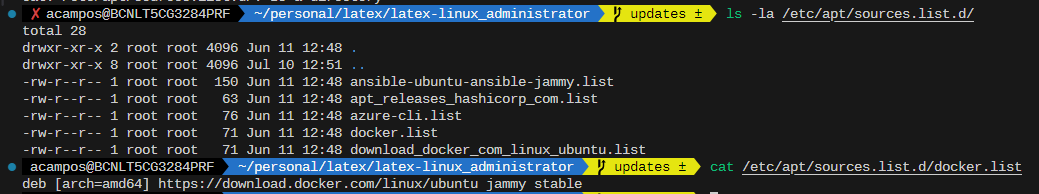
\includegraphics[width=\textwidth]{pictures/apt.png}
    \centering
\end{figure}

\begin{figure}[H]
    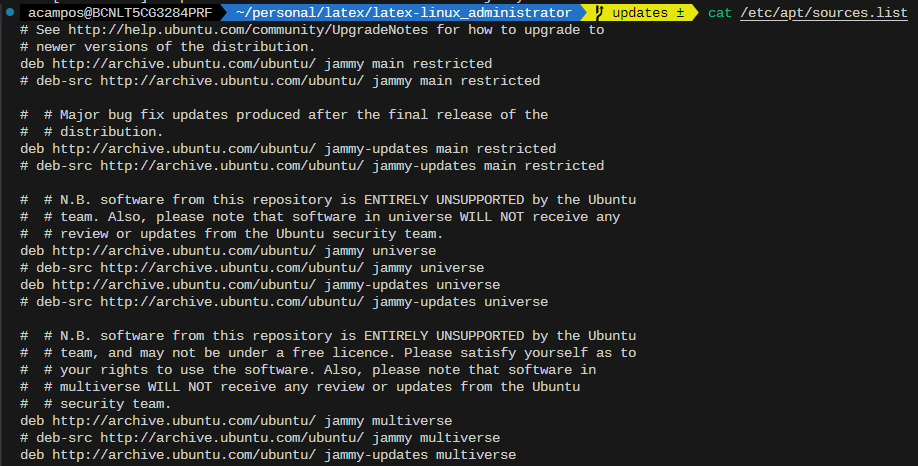
\includegraphics[width=\textwidth]{pictures/apt2.png}
    \centering
\end{figure}

When new repositories are added,  their GPG keys are fetched and added to the keyring \verb|/etc/apt/trusted.gpg.d/|. This ensures that APT can verify the integrity and authenticity of the packages from these repositories. 

By using /etc/apt/sources.list and /etc/apt/sources.list.d/, you can efficiently manage where your Ubuntu system looks for software packages and updates, ensuring that you have access to the latest and most secure versions of the software you need.

\begin{blocktemplateIII}{Warning}
However they can fuck up your \verb|apt update| because some of the repositories have been changed or the GPG key is not compatible. So you need to:
\begin{itemize}
    \item If the package is smart enough, just:
    \begin{itemize}
        \item \verb|sudo rm /etc/apt/sources.list.d/<package_name>.list|
        \item \verb|sudo apt-get update|
    \end{itemize}

    \item If not:
    \begin{itemize}
        \item \verb|sudo rm /etc/apt/sources.list.d/<package_name>.list|
        \item Add the new GPG key and install again the repository.
        \item \verb|sudo apt-get update|
    \end{itemize}
\end{itemize} 
\end{blocktemplateIII}

Repositories are added automagically, but to remove them:
\begin{codetemplate}
\begin{verbatim}
$ sudo rm /etc/apt/sources.list.d/<package_name>.list
\end{verbatim}
\end{codetemplate}

\subsection{Dnf - RedHat}

\subsubsection{Yum or Dnf?}
\textbf{Yum} (Yellowdog Updater, Modified) is an older package manager used for RPM-based distributions. It is known for its less efficient dependency resolution algorithm compared to \textbf{dnf}, which can result in slower performance, particularly with large repositories and metadata. While yum provides essential package management functions, it lacks some of the advanced features and flexibility found in dnf. However, it does offer backwards compatibility with older plugins and configurations, making it suitable for legacy systems.

On the other hand, \textbf{dnf} (Dandified Yum) is the modern successor to yum, introduced in Fedora 18 and later adopted by RHEL 8. It uses the libsolv library for faster and more efficient dependency resolution, significantly improving performance, especially with large repositories. dnf boasts advanced features, including better transaction handling, enhanced debugging capabilities, and improved support for extensions. It also supports modularity, allowing users to install different versions of software alongside each other. Despite its advancements, dnf maintains a high level of compatibility with yum commands, easing the transition for users.

\subsubsection{Basic dnf commands}
Update the local package index with the latest changes in the repositories:
\begin{codetemplate}
\begin{verbatim}
$ dnf check-update
\end{verbatim}
\end{codetemplate}

Upgrades all installed packages to the latest versions available in the repositories:
\begin{codetemplate}
\begin{verbatim}
$ dnf update
\end{verbatim}
\end{codetemplate}

Or which is the same:
\begin{codetemplate}
\begin{verbatim}
$ dnf upgrade
\end{verbatim}
\end{codetemplate}

Install the latest available version of a package:
\begin{codetemplate}
\begin{verbatim}
$ dnf install <package_name>
\end{verbatim}
\end{codetemplate}
    
Install a specific version of a package:
\begin{codetemplate}
\begin{verbatim}
$ dnf install <package_name>-<version>
\end{verbatim}
\end{codetemplate}

List all installed packages and their versions on the system:
\begin{codetemplate}
\begin{verbatim}
$ dnf list installed
\end{verbatim}
\end{codetemplate}

Look for specific package installed and its version:
\begin{codetemplate}
\begin{verbatim}
$ dnf list installed | grep <package_name>
\end{verbatim}
\end{codetemplate}

Look for the available versions of a package:
\begin{codetemplate}
\begin{verbatim}
$ dnf list --available <package-name>
\end{verbatim}
\end{codetemplate}
\begin{codetemplate}
\begin{verbatim}
$ dnf info <package-name>
\end{verbatim}
\end{codetemplate}
\begin{codetemplate}
\begin{verbatim}
$ dnf --showduplicates list <package-name>
\end{verbatim}
\end{codetemplate}

Update a specific package:
\begin{codetemplate}
\begin{verbatim}
$ dnf update <package_name>
\end{verbatim}
\end{codetemplate}

Remove a specific package and clean up depencencies:
\begin{codetemplate}
\begin{verbatim}
$ dnf remove package_name
\end{verbatim}
\end{codetemplate}
\begin{codetemplate}
\begin{verbatim}
$ dnf autoremove
\end{verbatim}
\end{codetemplate}

Remove unnecessary packages and dependencies:
\begin{codetemplate}
\begin{verbatim}
$ dnf autoremove
\end{verbatim}
\end{codetemplate}
\begin{codetemplate}
\begin{verbatim}
$ dnf clean all
\end{verbatim}
\end{codetemplate}

Check for broken dependencies:
\begin{codetemplate}
\begin{verbatim}
$ dnf check
\end{verbatim}
\end{codetemplate}

List enabled repositories:
\begin{codetemplate}
\begin{verbatim}
$ dnf repolist
\end{verbatim}
\end{codetemplate}

Enable/Disable Repositories:
\begin{codetemplate}
\begin{verbatim}
$ dnf config-manager --set-enabled <repository_id>
\end{verbatim}
\end{codetemplate}
\begin{codetemplate}
\begin{verbatim}
$ dnf config-manager --set-disabled <repository_id>
\end{verbatim}
\end{codetemplate}

\newpage
%-------------------------------------------------------------------------------------------------
\section{.bashrc, .bash\_profile, /etc/bashrc \& path}

\subsection{.bashrc vs .bash\_profile}

\begin{itemize}
    \item \verb|.bashrc| \textbf{[non interactive login]:} for changes to take effect, we need to open another interactive terminal (changes don't apply to the current one because this file is executed upon starting a new terminal session).
    \item \verb|.bash_profile| \textbf{[interactive login]:} it only executes when there's a login process, upon restarting the machine, when using ssh, sudo... But not when opening a new terminal.
\end{itemize}

\subsection{PATH}
\textbf{PATH} is an environmental variable in Linux that \textbf{tells the shell which directories to search for executable files} (i.e., ready-to-run programs) in response to commands issued by a user.

When you type a command into the command prompt in Linux, all you're doing is telling it to run a program. Even simple commands, like ls, mkdir, rm, and others are just small programs that usually live inside a directory on your computer called \verb|/usr/bin|. Other places to search for executables: \verb+/usr/local/bin+, \verb+/usr/local/sbin+, and \verb+/usr/sbin+. 

When you type a command into your Linux shell, it doesn't look in every directory to see if there's a program by that name. It only looks to the ones you specified in the \verb|$PATH| environment var.

Sometimes, you may wish to install programs into other locations on your computer, but be able to execute them easily without specifying their exact location. You can do this easily by adding a directory to your \verb|$PATH|.

View your PATH
\begin{codetemplate}{}
\begin{verbatim}
$ echo $PATH
\end{verbatim}
\end{codetemplate}

\subsection{Set your PATH}
\subsubsection{For current terminal}
\begin{codetemplate}{}
\begin{verbatim}
$ export PATH=$PATH:/place/to/the/binary/file
\end{verbatim}
\end{codetemplate}

\subsubsection{Permanently for interactive sessions}

But what happens if you restart your computer or create a new terminal instance? Your addition to the path is gone! This is by design. The variable \verb|$PATH| is set by your shell every time it launches. The exact way to do this depends on which shell you're running.

Add the following line to \verb|~/.bash_profile|, \verb|~/.bashrc|, or \verb|/.profile|

\begin{codetemplate}{}
\begin{verbatim}
$ export PATH=\$PATH:/place/with/the/file
\end{verbatim}
\end{codetemplate}

\begin{blocktemplateIII}{Nota}
Be very careful editing these files, so one error in the configuration of these files can make somo binaries crash (example: mkdir, ls, etc.)
\end{blocktemplateIII}

\newpage
%-------------------------------------------------------------------------------------------------
\section{Useful Tools}

\subsection{Cat}
Cat will allow us to view the contents of files without opening them, create files if they do not exist or redirect terminal outputs.

\begin{itemize}
    \item \textbf{Basic usage:} show the content of a file
\begin{codetemplate}{}
\begin{verbatim}
$ cat test
\end{verbatim}
\end{codetemplate}

    \item Show the content of both files test and test2
\begin{codetemplate}{}
\begin{verbatim}
$ cat test1 test2
\end{verbatim}
\end{codetemplate}

    \item Adds the content of test2 to the file test1, if there was content it overwrites, if there was nothing, it creates the new file
\begin{codetemplate}{}
\begin{verbatim}
$ cat test1 > test2
\end{verbatim}
\end{codetemplate}

    \item Appends the content of test2 into the file test1, if there is no test2, it will create it
\begin{codetemplate}{}
\begin{verbatim}
$ cat test1 >> test2
\end{verbatim}
\end{codetemplate}

    \item Show line number
\begin{codetemplate}{}
\begin{verbatim}
$ cat -n file
\end{verbatim}
\end{codetemplate}

    \item \textbf{Writte in a file the content we want, as we were with text editor} (Exit: Ctrl+D)
\begin{codetemplate}{}
\begin{verbatim}
$ cat > filename
\end{verbatim}
\end{codetemplate}
\end{itemize}

\begin{figure}[H]
    \centering
    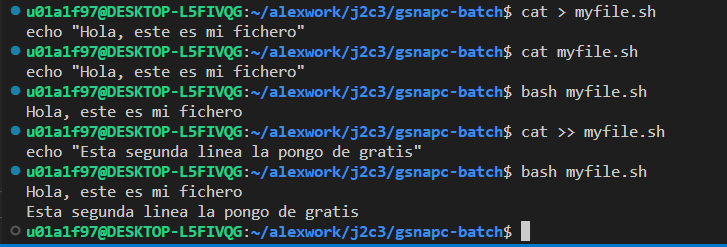
\includegraphics[scale=0.7]{pictures/image1.png}
    \caption{amazing cat}
\end{figure}

\subsection{Head \& Tail}

\textbf{Head:} print the first 10 lines of each FILE to standard output

\begin{itemize}
    \item Print the first NUM lines instead of the first 10
\begin{codetemplate}{}
\begin{verbatim}
$ head -n <number_of_lines> <filename>
\end{verbatim}
\end{codetemplate}
\end{itemize}

\textbf{Tail:}  print the last 10 lines of each FILE to standard output.

\begin{itemize}
    \item Print the last NUM lines instead of the last 10
\begin{codetemplate}{}
\begin{verbatim}
$ head -n <number_of_lines> <filename>
\end{verbatim}
\end{codetemplate}

    \item Attach the terminal following the evolution of the file
\begin{codetemplate}{}
\begin{verbatim}
$ head -f <filename>
\end{verbatim}
\end{codetemplate}
\end{itemize}

\subsection{Diff (File comparator)}
Command to compare FILES line by line.

\textbf{Basic usage}
\begin{codetemplate}{}
\begin{verbatim}
$ diff main.py main_old.py
\end{verbatim}
\end{codetemplate}

\textbf{Report only when files differ}
\begin{codetemplate}{}
\begin{verbatim}
$ diff -q ...
\end{verbatim}
\end{codetemplate}

\textbf{Report when two files are the same}
\begin{codetemplate}{}
\begin{verbatim}
$ diff -s ...
\end{verbatim}
\end{codetemplate}

\textbf{Ignore case}
\begin{codetemplate}{}
\begin{verbatim}
$ diff -i ...
\end{verbatim}
\end{codetemplate}

\textbf{Ignore changes in the amount of white space}
\begin{codetemplate}{}
\begin{verbatim}
$ diff -b ...
\end{verbatim}
\end{codetemplate}

\textbf{Ignore all white space}
\begin{codetemplate}{}
\begin{verbatim}
$ diff -w ...
\end{verbatim}
\end{codetemplate}

\textbf{Ignore changes where lines are all blank}
\begin{codetemplate}{}
\begin{verbatim}
$ diff -B ...
\end{verbatim}
\end{codetemplate}

\textbf{Output NUM (default 3) lines of copied contex}
\begin{codetemplate}{}
\begin{verbatim}
$ diff -c ...
\end{verbatim}
\end{codetemplate}

\textbf{Output side by side (2 columns)}
\begin{codetemplate}{}
\begin{verbatim}
$ diff -y ...
\end{verbatim}
\end{codetemplate}

\subsection{Grep (Global search for Regular Expressions and Print out)}

\begin{blocktemplate}{Nota}
grep, egrep, fgrep, rgrep - print lines that match patterns.
In addition, the variant programs egrep, fgrep and rgrep are the same as grep -E, grep -F, and grep -r, respectively.  These variants are deprecated, but are provided for backward compatibility.
\end{blocktemplate}

\subsubsection{Two flavors of grep usage}
\begin{enumerate}
    \item \textbf{Use grep to search text in a file / files}
\begin{codetemplate}{}
\begin{verbatim}
$ grep "texto-buscado" <archivo/archivos>
\end{verbatim}
\end{codetemplate}

    \item \textbf{Use grep to search text in the Terminal STDOUT}
\begin{codetemplate}{}
\begin{verbatim}
$ COMMAND [args...] | grep "texto-buscado"
\end{verbatim}
\end{codetemplate}
\end{enumerate}
The result of this is the occurrences of the pattern (by the line it is on) in the / stdout files. If there is no match, no output will be printed to the terminal.

\begin{blocktemplateII}{Note}
    The "" are necessary to convert to String. If what we introduce is already a String, they would not be necessary. Example:
\begin{itemize}
    \item \verb|grep alias file.txt|: We dont need ""
    \item \verb|grep "alias pepito" file.txt|: We need ""
\end{itemize}
\end{blocktemplateII}

\subsubsection{Useful Flags}

\textbf{line Number}
\begin{codetemplate}{}
\begin{verbatim}
$ grep -n ...
\end{verbatim}
\end{codetemplate}

\textbf{Count the number of coincident lines}
\begin{codetemplate}{}
\begin{verbatim}
$ grep -c ...
\end{verbatim}
\end{codetemplate}

\textbf{IgnoreCase}
\begin{codetemplate}{}
\begin{verbatim}
$ grep -i ...
\end{verbatim}
\end{codetemplate}

\textbf{Execute in silent mode, suppress all normal output}
\begin{codetemplate}{}
\begin{verbatim}
$ grep -q ...
\end{verbatim}
\end{codetemplate}

\textbf{Accept extended regular expressions}
\begin{codetemplate}{}
\begin{verbatim}
$ grep -E ...
\end{verbatim}
\end{codetemplate}

\textbf{Use PATTERNS for matching, you can specify multiple patterns to search for}
\begin{codetemplate}{}
\begin{verbatim}
$ grep -e 'pattern1' -e 'pattern2' file.txt
\end{verbatim}
\end{codetemplate}

\textbf{Match only full words}
\begin{codetemplate}{}
\begin{verbatim}
$ grep -w
\end{verbatim}
\end{codetemplate}

\textbf{Match only full lines}
\begin{codetemplate}{}
\begin{verbatim}
$ grep -x
\end{verbatim}
\end{codetemplate}

\textbf{Print non-matching liness}
\begin{codetemplate}{}
\begin{verbatim}
$ grep -v
\end{verbatim}
\end{codetemplate}

\textbf{Before Context or Aftercontext}
\begin{codetemplate}{}
\begin{verbatim}
$ grep "text" file -A NUMBER_A -B NUMBER_B
\end{verbatim}
\end{codetemplate}


\textbf{Recursive Search}
By default, grep cannot search for directories. If you try to do so, you will get an error ("It is a directory"). With the -R option, searching for files across directories and subdirectories becomes possible.
\begin{codetemplate}{}
\begin{verbatim}
$ grep -R
\end{verbatim}
\end{codetemplate}

\textbf{Print only names of FILEs with selected lines}
\begin{codetemplate}{}
\begin{verbatim}
$ grep -l
\end{verbatim}
\end{codetemplate}

\textbf{Print only names of FILEs with no selected lines}
\begin{codetemplate}{}
\begin{verbatim}
$ grep -L
\end{verbatim}
\end{codetemplate}


\subsection{Find}

Command to search for files in a directory hierarchy.


\textbf{Find all files and directories from "/" with the name "linux"}
\begin{codetemplate}{}
\begin{verbatim}
$ find / -name "linux"
\end{verbatim}
\end{codetemplate}

\textbf{Find all files and directories from "/" with the name "linux" and list them}
\begin{codetemplate}{}
\begin{verbatim}
$ find / -name "linux" -ls
\end{verbatim}
\end{codetemplate}

\textbf{Find just files"}
\begin{codetemplate}{}
\begin{verbatim}
$ find / -type f -name "linux"
\end{verbatim}
\end{codetemplate}

\textbf{Find just directories"}
\begin{codetemplate}{}
\begin{verbatim}
$ find / -type d -name "linux"
\end{verbatim}
\end{codetemplate}

\textbf{Find from our current directory all the files which name contains the substring "Thr"}
\begin{codetemplate}{}
\begin{verbatim}
$ find . -name "*Thr*" 
\end{verbatim}
\end{codetemplate}

\begin{figure}[H]
    \centering
    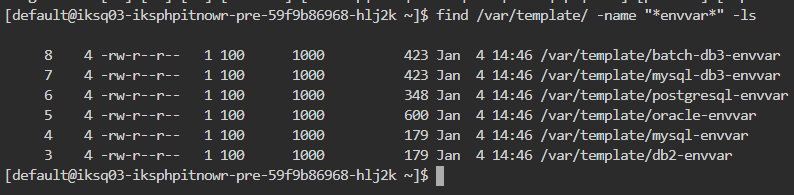
\includegraphics[scale=0.7]{pictures/image3.png}
    \caption{use of find}
\end{figure}

\begin{blocktemplateII}{NOTE}
The "" are optional, because they are just to define strings (process spaces and weird characters as part of the string)
\end{blocktemplateII}


\subsection{Sed (Stream Editor)}

 It is a very essential tool for text processing, specifically it is common used for text replacement. Con Sed podemos editar archivos, incluso sin abrirlos, de manera individual o masiva. Dicho sea, que esta forma, es mucho más rápida para encontrar y reemplazar algo en un archivo de manera manual.

 Print the content of "fichero.txt" replacing the first occurrence of the string "Microsoft Windows" by "GNU Linux" in the file "fichero.txt"
\begin{codetemplate}{}
\begin{verbatim}
$ sed "s/Microsoft Windows/GNU Linux/" fichero.txt
\end{verbatim}
\end{codetemplate}

Save the changes in the file:
\begin{codetemplate}{}
\begin{verbatim}
$ sed -i "s/Microsoft Windows/GNU Linux/" fichero.txt
\end{verbatim}
\end{codetemplate}

 Replace all the occurrences of the string "Microsoft Windows" by "GNU Linux" in the file "fichero.txt" and save.
 \begin{codetemplate}{}
\begin{verbatim}
$ sed -i "s/Microsoft Windows/GNU Linux/g" fichero.txt
\end{verbatim}
\end{codetemplate}

 Replace just the 3rd occurrence of "Microsoft Windows" by "GNU Linux" in the text and save
\begin{codetemplate}{}
\begin{verbatim}
$ sed "s/Microsoft Windows/GNU Linux/3g" fichero.txt
\end{verbatim}
\end{codetemplate}

Replace the string "Microsoft Windows" just in line 1:
\begin{codetemplate}{}
\begin{verbatim}
$ sed "1 s/Microsoft Windows/GNU Linux/" fichero.txt
\end{verbatim}
\end{codetemplate}

\begin{blocktemplate}{NOTE}
By default sed is \textbf{case SENSITIVE} but to change it by case insensitive, you can add \verb|I| at the end of the REGEX:
 \begin{codetemplate}{}
\begin{verbatim}
$ sed -i "s/Microsoft Windows/GNU Linux/gI" fichero.txt
\end{verbatim}
\end{codetemplate}
\end{blocktemplate}

\begin{blocktemplateIII}{WARNING}
Sed will replace all the string matches, without differentiating if it is completed or partial, for example:
\begin{figure}[H]
    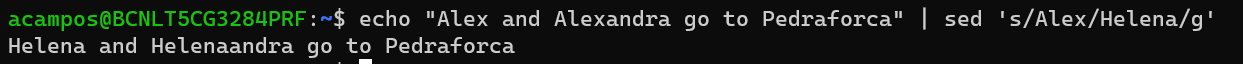
\includegraphics[width=\textwidth]{pictures/sed.png}
    \centering
\end{figure}

To replace the exact match you should use spaces, \textbf{in REGEX} \verb|space=\s|:
\begin{codetemplate}{}
\begin{verbatim}
$ sed "s/Alex\s/Claudia /g"
\end{verbatim}
\end{codetemplate}
\end{blocktemplateIII}

For more information:
\href{https://www.ochobitshacenunbyte.com/2019/05/28/uso-del-comando-sed-en-linux-y-unix-con-ejemplos/}{Uso del Comando Sed} 

\subsection{AWK}
Powerful text processing tool in Linux and Unix environments. It's primarily used for pattern scanning and processing. awk reads input line by line and divides each line into fields (by default, using whitespace as the delimiter). You can then specify patterns and actions to perform on those patterns.

\textbf{Basic:} Perform an action in the lines that match the pattern in the file
\begin{codetemplate}{}
\begin{verbatim}
$ awk '/pattern/ { action }' <filename>
\end{verbatim}
\end{codetemplate}

\textbf{Print the first field of each line in the file (separated by default by space)}
\begin{codetemplate}{}
\begin{verbatim}
$ awk '{ print $1 }' <filename>
\end{verbatim}
\end{codetemplate}

\textbf{Print the 3rd field of each line in the file (separated by ":")}
\begin{codetemplate}{}
\begin{verbatim}
$ awk -F ":" '{ print $3 }' <filename>
\end{verbatim}
\end{codetemplate}

\textbf{Print specific fields of each line in the file (separated by ":")}
\begin{codetemplate}{}
\begin{verbatim}
$ awk -F ":" '{ print $2, $3 }' <filename>
\end{verbatim}
\end{codetemplate}

\subsection{Tar Command}
The tar command on Linux is often used to create .tar.gz or .tgz archive files, or extract them into local directories.
\subsubsection{Compress}
\textbf{Basics}
\newline
Use the following command to compress an entire directory or a single file on Linux. It’ll also compress every other directory inside a directory you specify–in other words, it works recursively.
\begin{codetemplate}{}
\begin{verbatim}
$ tar -czvf name-of-archive.tar.gz /path/to/directory-or-file
\end{verbatim}
\end{codetemplate}

\textbf{Compress multiple files/directories in a unique archive}
\begin{codetemplate}{}
\begin{verbatim}
$ tar -czf FILENAME.tar.gz path/to/dir1 path/to/file1 path/to/dir2 ...
\end{verbatim}
\end{codetemplate}

\textbf{Exclude files or directories}
\begin{codetemplate}{}
\begin{verbatim}
$ tar -czf FILENAME.tar.gz path/to/dir1 \
--exclude=/path/to/dir1/excludeddir \
path/to/dir2 --exclude=/path/to/dir1/*.mp4
\end{verbatim}
\end{codetemplate}

\subsubsection{Extract}
\textbf{Basics}
\newline
Once you have an archive, you can extract it with the tar command. The following command will extract the contents of archive.tar.gz to the current directory.
\begin{codetemplate}{}
\begin{verbatim}
$ tar -xzvf archive.tar.gz
\end{verbatim}
\end{codetemplate}
\textbf{Choose the extract directory}
\newline
You may want to extract the contents of the archive to a specific directory. You can do so by appending the -C switch to the end of the command:
\begin{codetemplate}{}
\begin{verbatim}
$ tar -xzvf archive.tar.gz -C /path/to/directory/to/extract
\end{verbatim}
\end{codetemplate}

More information in: \href{https://www.howtogeek.com/248780/how-to-compress-and-extract-files-using-the-tar-command-on-linux/}{How-To Geek tar}

Here’s what those switches actually mean:

\begin{itemize}
    \item \textbf{-c:} \textbf{c}reate an archive
    \item \textbf{-z:} compress into g\textbf{z}ip
    \item \textbf{-v:} \textbf{v}erbose [removable]
    \item \textbf{-f:} allows you to specify the FILENAME \textbf{filename} of archive
\end{itemize}

\begin{blocktemplateIII}{Nota}
-f switch must be the last one, because is the flag which specifies the name of the file indicated after.
\end{blocktemplateIII}

\subsubsection{More flags}
\begin{itemize}
    \item \textbf{-x:} Extract the archive 
    \item \textbf{-t:} displays or lists files in archived file 
    \item \textbf{-u:} archives and adds to an existing archive file 
    \item \textbf{-A:} concatenates the archive files 
    \item \textbf{-j:} filter archive tar file using tbzip
    \item \textbf{-W:} verify a archive file
    \item \textbf{-r:} update or add file or directory in already existed .tar file
\end{itemize}

\subsection{Base64 Encoding}

Base64 encode or decode FILE, or standard input, to standard output.

\textbf{Code}
\begin{codetemplate}{}
\begin{verbatim}
$ echo -n $PASSWORD_CLEAR | base64
\end{verbatim}
\end{codetemplate}

\textbf{Decode}
\begin{codetemplate}{}
\begin{verbatim}
$ echo -n $PASSWORD_CODED | base64 -d
\end{verbatim}
\end{codetemplate}

\begin{figure}[H]
    \centering
    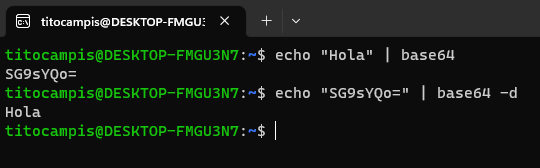
\includegraphics[width=\textwidth]{pictures/base64.png}
\end{figure}


\subsection{JQ}

To parse into a beatufiul json format:
\begin{codetemplate}{}
\begin{verbatim}
$ cat file.json | jq "."
\end{verbatim}
\end{codetemplate}

To show the content inside field in a beatufiul json format:
\begin{codetemplate}{}
\begin{verbatim}
$ cat file.json | jq ".field"
\end{verbatim}
\end{codetemplate}

\subsection{YQ}

Is the same as \textbf{jq} but to parse YAML files.

For more information, check \url{https://github.com/mikefarah/yq}

\newpage
%-------------------------------------------------------------------------------------------------
\section{Linux Default Text Editors}
\subsection{Vi}
Vi (VIsual editor) is the default editor that comes with the UNIX operating system. It is is a full screen editor and has two modes of operation:

\begin{itemize}
    \item \textbf{Command mode:} mode to write shortcurts which cause action to be taken on the file, as remove line, save, undo, redo, etc.
    \item \textbf{Insert mode:} mode which entered text is directly inserted into the file.
\end{itemize}

We are not going to dedicate more time to \textbf{vi}, because it is actually not used. Instead of \textbf{vi}, \textbf{vim} is used (Vi IMproved). Which we are going to analize in the next section.

\subsection{Vim}

\subsubsection{Introduction}

Vim (Vi IMproved) is an enhanced version of the original Vi editor, it builds upon the features of Vi while adding numerous enhancements and improvements. These enhancements include syntax highlighting, built-in support for scripting, extensive customizability, plugin support, portability and many additional commands and options.

While Vi is still used and appreciated for its simplicity and efficiency, Vim has become the de facto standard for many developers and system administrators due to its enhanced features and flexibility.

As well as vi, it has two modes of operation:

\begin{itemize}
    \item \textbf{Command mode:} mode to write shortcurts which cause action to be taken on the file, as remove line, save, undo, redo, etc.
    \item \textbf{Insert mode:} mode which entered text is directly inserted into the file.
\end{itemize}

When you enter vim, you enter in the \textbf{command mode}, so to change to the \textbf{insert mode}:

\begin{codetemplate}{}
\begin{verbatim}
i
\end{verbatim}
\end{codetemplate}

To go from \textbf{insert mode} to the \textbf{command mode}:
\begin{codetemplate}{}
\begin{verbatim}
Esc
\end{verbatim}
\end{codetemplate}

\subsubsection{Command Mode Shortcuts}

\textbf{Exit:}

\begin{itemize}
    \item Without save the changes
\begin{codetemplate}{}
\begin{verbatim}
:q!
\end{verbatim}
\end{codetemplate}
    \item Saving the changes
\begin{codetemplate}{}
\begin{verbatim}
:q
\end{verbatim}
\end{codetemplate}

    \item Forcing to save the changes
\begin{codetemplate}{}
\begin{verbatim}
:wq
\end{verbatim}
\end{codetemplate}
\end{itemize}


Undo
\begin{codetemplate}{}
\begin{verbatim}
u
\end{verbatim}
\end{codetemplate}

Redo
\begin{codetemplate}{}
\begin{verbatim}
r
\end{verbatim}
\end{codetemplate}
\begin{codetemplate}{}
\begin{verbatim}
Ctrl+r # On INSERT mode
\end{verbatim}
\end{codetemplate}

Remove a full line
\begin{codetemplate}{}
\begin{verbatim}
dd
\end{verbatim}
\end{codetemplate}

To remove the current word
\begin{itemize}
    \item With the spaces:
\begin{codetemplate}
\begin{verbatim}
daw
\end{verbatim}
\end{codetemplate}
    \item Without the spaces:
\begin{codetemplate}
\begin{verbatim}
diw
\end{verbatim}
\end{codetemplate}
\end{itemize}


Find occurrences
\begin{codetemplate}
\begin{verbatim}
/<words>
\end{verbatim}
\end{codetemplate}
\begin{itemize}
    \item To start finding the occurrences: Intro
    \item To go to the next occurrence: n
    \item \textbf{By dafault it is case sensitive, to make it insensitive:} before search, execute.
\begin{codetemplate}
\begin{verbatim}
:set ignorecase
\end{verbatim}
\end{codetemplate}
    \item To replace the first occurrence of a word
\begin{codetemplate}
\begin{verbatim}
:s/search/replace/
\end{verbatim}
\end{codetemplate}
    \item To replace all the occurrences of a word in the full file
\begin{codetemplate}
\begin{verbatim}
:%s/search/replace/g
\end{verbatim}
\end{codetemplate}
    item To replace all the occurrences of a word in the full file (with confirmation before each replacement)
\begin{codetemplate}
\begin{verbatim}
:%s/search/replace/gc
\end{verbatim}
\end{codetemplate}
\end{itemize}

Go to the start of the current line
\begin{codetemplate}
\begin{verbatim}
0
\end{verbatim}
\end{codetemplate}

Go to the end of the current line
\begin{codetemplate}
\begin{verbatim}
$
\end{verbatim}
\end{codetemplate}

Go to the beginning of the current line
\begin{codetemplate}
\begin{verbatim}
gg
\end{verbatim}
\end{codetemplate}

Go to the end of the current line
\begin{codetemplate}
\begin{verbatim}
G
\end{verbatim}
\end{codetemplate}

To configure the colors of the terminal
\begin{codetemplate}
\begin{verbatim}
:scolorscheme <name_of_scheme>
\end{verbatim}
\end{codetemplate}

\subsubsection{Vim Config}

\begin{codetemplate}{}
\begin{verbatim}
$ sudo vim ~/.vimrc
\end{verbatim}
\end{codetemplate}

\begin{codetemplate}{}
\begin{verbatim}
" Disable compatibility with vi which can cause unexpected issues.
set nocompatible

" Enable type file detection. Vim will be able to try to detect the type of file in use.
filetype on

" Enable plugins and load plugin for the detected file type.
filetype plugin on

" Load an indent file for the detected file type.
filetype indent on

" Set authomatic indentation
" set autoindent

" Turn syntax highlightin
syntax on

" Add numbers to each line on the left-hand side.
set number

" Highlight cursor line underneath the cursor horizontally.
set cursorline

" Highlight cursor line underneath the cursor vertically.
set cursorcolumn

" Set shift width to 4 spaces.
set shiftwidth=4

" Set tab width to 4 columns.
set tabstop=4

" Use space characters instead of tabs.
set expandtab

" Colorful (),[],{}
set showmatch

" While searching though a file incrementally highlight matching characters as you type.
set incsearch

" Ignore capital letters during search.
set ignorecase

" Use highlighting when doing a search.
set hlsearch

" Enable auto completion menu after pressing TAB.
set wildmenu

" Make wildmenu behave like similar to Bash completion.
set wildmode=list:longest

" Enable black theme
" set background=dark

" Tab helper
" set smarttab
\end{verbatim}
\end{codetemplate}

If you want to persistthis configuration when using \verb|sudo vim| you will need to do something a little bit tricky:

\begin{itemize}
    \item Create an alias in your \verb|~/.bashrc| file:
\begin{codetemplate}{}
\begin{verbatim}
alias svim="sudo -E vim"
\end{verbatim}
\end{codetemplate}

    \item Use always
\begin{codetemplate}{}
\begin{verbatim}
$ svim <file>
\end{verbatim}
\end{codetemplate}
\end{itemize}

\subsection{Nano}
Nano is a simple and easy-to-use text editor for Unix-like operating systems. It's especially popular among beginners due to its straightforward interface and command set. Unlike more complex editors like Vim or Emacs, Nano provides an intuitive environment where users can create and edit files without a steep learning curve. It features on-screen command reminders, which make it accessible for those who are new to command-line text editing.

Save the file
\begin{codetemplate}{}
\begin{verbatim}
Ctrl + O
\end{verbatim}
\end{codetemplate}

Exit Nano
\begin{codetemplate}{}
\begin{verbatim}
Ctrl + X
\end{verbatim}
\end{codetemplate}

Undo the last operation
\begin{codetemplate}{}
\begin{verbatim}
Alt + U
\end{verbatim}
\end{codetemplate}

Redo the last operation
\begin{codetemplate}{}
\begin{verbatim}
Alt + E
\end{verbatim}
\end{codetemplate}

Search within the file
\begin{codetemplate}{}
\begin{verbatim}
Ctrl + W
\end{verbatim}
\end{codetemplate}

Search and replace within the file
\begin{codetemplate}{}
\begin{verbatim}
Ctrl + \
\end{verbatim}
\end{codetemplate}

Cut the current line
\begin{codetemplate}{}
\begin{verbatim}
Ctrl + K
\end{verbatim}
\end{codetemplate}

Paste the current line
\begin{codetemplate}{}
\begin{verbatim}
Ctrl + U
\end{verbatim}
\end{codetemplate}

Move to the begining of the current line
\begin{codetemplate}{}
\begin{verbatim}
Ctrl + A
\end{verbatim}
\end{codetemplate}

Move to the end of the current line
\begin{codetemplate}{}
\begin{verbatim}
Ctrl + E
\end{verbatim}
\end{codetemplate}

Move to the begining of the file
\begin{codetemplate}{}
\begin{verbatim}
Alt + ^
\end{verbatim}
\end{codetemplate}

Move to the end of the file
\begin{codetemplate}{}
\begin{verbatim}
Alt + $
\end{verbatim}
\end{codetemplate}

Delete the current word
\begin{codetemplate}{}
\begin{verbatim}
Alt + D
\end{verbatim}
\end{codetemplate}


\newpage
%-------------------------------------------------------------------------------------------------
\section{Network}

\subsection{OSI Model}

The Open Systems Interconnection (OSI) model is a reference model from the International Organization for Standardization (ISO) that "provides a common basis for the coordination of standards development for the purpose of systems interconnection. In the OSI reference model, the communications between systems are split into seven different abstraction layers: Physical, Data Link, Network, Transport, Session, Presentation, and Application.

\begin{figure}[H]
    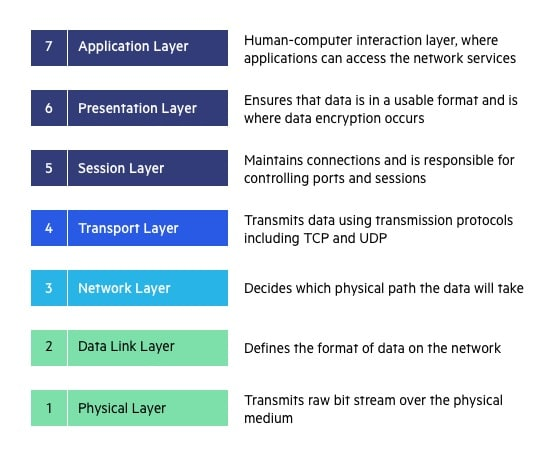
\includegraphics[scale=0.6]{pictures/OSI-7-layers.jpg}
    \centering
\end{figure}

\subsection{MAC Adress vs IP Address}

\subsubsection{Introduction}

Suppose someone has to deliver a package to someone else. To effectively send the courier, the sender must provide two details about the recipient. The two items are the receiver's name and address, which may include a house number, street, city, state, and pin code (to identify the right person to deliver the courier specifically). If we apply this example to networking, the MAC address will be the address of the particular node where we want to send the data, and the IP address will be the address of the network connection where several devices may be present.

A MAC address and an IP address both help identify a device specifically on the internet. The IP address is generated by the ISP (Internet Service Provider), whereas the MAC address is provided by the Network Interface Controller (NIC)manufacturer. There are significant differences between a MAC address and an IP address. The IP address of a device is crucial for determining a network's connection (using which the device is connecting to the network). On the other hand, the MAC address guarantees the computer device's precise location. It enables us to uniquely identify a certain device on the access network.

Every device connected to a network has a Media Access Control (MAC) address that uniquely identifies it, much like every house has a unique postal address. Meanwhile IP addresses are just as significant as a person's identification number or card. 

\subsubsection{MAC Address (Media Control Address)}

A MAC address, which is also known as a hardware or physical address, is an unique alphanumeric identifier consisting of 12 characters. MAC address is allocated to a network interface controller (NIC) and functions as a network address when communications occur within a network segment. Ethernet, Wi-Fi, and Bluetooth are just a few of the IEEE 802 networking technologies that frequently employ this application. Six groups of two hexadecimal digits between 00 and FF (48 bits in length) constitute MAC addresses. They can be separated by ":", "-", ",", " " or not separated at all. An example of MAC address:
\begin{itemize}
    \item 02:AB:6D:9C:EF:42
    \item 02-AB-6D-9C-EF-42
    \item 02 AB 6D 9C EF 42
\end{itemize}

The first 24 bits of the MAC address, the first 3 octets (first 3 hexadecimal groups) are the ID number of the adapter manufacturer, here we have examples of OUIs (Organisationally Unique Identifier):

\begin{itemize}
    \item \textbf{Cisco:} CC:46:D
    \item \textbf{Google:} 3C:5A:B4 
    \item \textbf{HP:} 3C:D9:2B
    \item \textbf{Intel:} 00:A0:C9
\end{itemize}

The serial number that the manufacturer assigned to the adapter is represented by the second half of a MAC address (24 more bits)

\begin{figure}[H]
    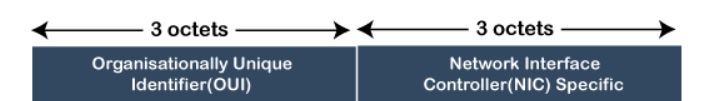
\includegraphics[width=\textwidth]{pictures/mac.png}
    \centering
\end{figure}

MAC address  operate at the Data Link Layer (Layer 2) of the OSI model. They are used to identify devices within a local network (LAN). It is unique: every network interface card (NIC) is assigned a unique MAC address by the manufacturer, ensuring that no two devices on the same network have the same MAC address.

Within a local network, devices communicate with each other using MAC addresses. For instance, when a device wants to send data to another device on the same network, it uses the destination device's MAC address. As it is operating at OSI Layer 2, data is encapsulated into Ethernet frames, which include the source and destination MAC addresses.

\textbf{How to know my MAC address?}


Windows (powershell): execute the following command and look for the "Physical Address" under the network adapter you're using. 
\begin{codetemplate}{}
\begin{verbatim}
$ ipconfig /all
\end{verbatim}
\end{codetemplate}

Linux: execute the following command and check for ethX for Ethernet or wlanX for Wi-Fi
\begin{codetemplate}{}
\begin{verbatim}
$ ip addr
\end{verbatim}
\end{codetemplate}

Router, Mobile, Windows (without terminal), Linux (without terminal): check the device configuration.

\subsubsection{IP Address}

The term "Internet Protocol", for which the abbreviation IP stands, is a set of guidelines that control the format of data exchanged via a local or public network.

An IP address is an identification tool for network connections. A link in a network receives what is known as a "logical address" from the network. IP addresses define how internet routers behave and allow you to regulate how devices communicate over the Internet.

An internet protocol address (IP address) is a numerical representation of a network interface that serves as its sole means of identification such as 192.97.23.57.

The two IP versions that are now in use are IPv4 and IPv6. The original IPv4 protocol is still in use today on the internet and in many corporate networks. On the other hand, the IPv4 protocol was limited to $2^{32}$ addresses. Due to the way addresses were assigned, there would be a situation where there wouldn't be enough unique addresses for all internet-connected devices. That's why the most recent version is Internet Protocol version 6 (IPv6). To accommodate the demand for more Internet addresses, this new IP address version is being used. It was developed to overcome IPv4 issues. With a 128-bit address space, it supports 340 billion distinct address spaces. IPng (Internet Protocol next generation) is another name for IPv6.

An IP address is used to manage the connection between gadgets that send and receive data over a network. Without an IP address, it is impossible to communicate with any device connected to the internet. IP addresses allow computing devices (such PCs and tablets) to communicate with websites and streaming services, as well as information websites of the identity of the connecting user.

IP Address works operate at the Network Layer (Layer 3) of the OSI model. They are used for logical addressing and routing of packets across different networks, including the global internet, so data is encapsulated into IP packets, which include the source and destination IP addresses.

\subsubsection{Why Both MAC and IP Addresses Are Needed}

Having both MAC and IP addresses allows for the separation of physical hardware identification (MAC) from logical network addressing (IP). This separation simplifies network management, mobility, and security. 

Devices can move between networks and retain their unique MAC address, while their IP address can change based on the network they are connected to. This flexibility supports mobile devices and scalable network architectures.

\textbf{Local vs Global Scope:}
\begin{itemize}
    \item \textbf{MAC Address:} Used for communication within a local network segment (Layer 2). It is essential for Ethernet communication and ensures that data reaches the correct device on the same network.
    \item \textbf{IP Address:} Used for communication between different networks (Layer 3). It enables data to be routed across the internet and large networks.
\end{itemize}

\textbf{Routing and Address Resolution:}

\begin{itemize}
    \item \textbf{Routing:} IP addresses are used by routers to make forwarding decisions and route data across multiple networks to its final destination.
    \item \textbf{Address Resolution Protocol (ARP):} When a device wants to communicate with another device on the same local network, it uses ARP to map the destination IP address to the corresponding MAC address. This mapping is necessary because data frames on Ethernet networks require MAC addresses.
\end{itemize}

\subsection{Public IP}

\subsubsection{Introduction}
A public IP address uniquely identifies your network on the internet. It allows other networks and devices on the internet to locate and communicate with your network. When you send data over the internet (e.g., browsing websites, streaming videos), it needs a destination and return path. The public IP address serves as the return address for the data requested by devices within your local network.

The Public IP is set at router level, not at device level, and any time you access a website, your request is sent from your device to your router, which then uses the public IP address to send the request out to the internet. The response from the website is sent back to your router's public IP address, which then routes the response back to your device and vice versa.

The router uses NAT to translate private IP addresses (used within your local network) into the public IP address. This allows multiple devices on your local network to share a single public IP address for accessing the internet.

So if you host a service (e.g., a web server) on a device on your network, you will need to define a NAT route in your router in order to other devices on the internet use your public IP to connect to your server.

\subsubsection{How to get my public ip?}

I can do it with different methods:

\begin{codetemplate}{}
\begin{verbatim}
$ curl ifconfig.me
\end{verbatim}
\end{codetemplate}

\begin{codetemplate}{}
\begin{verbatim}
$ dig +short myip.opendns.com @resolver1.opendns.com
\end{verbatim}
\end{codetemplate}

Each of these commands contacts an external service that echoes back your public IP address. This IP address is what others on the internet see as your point of contact.

\subsubsection{Who is this IP assigned to me?}

Your router's public IP address is assigned by your Internet Service Provider (ISP). Usually, if your IP is not for bussiness or point to point specific connection, in which case the assignment of the IP is static. The assignment of the IP is dynamic using DHCP.

The dynamic IP Address Assignment using DHCP works like folowing:

\begin{enumerate} 
    \item Your ISP uses Dynamic Host Configuration Protocol (DHCP) to assign IP addresses. This means that your router is given a dynamic public IP address from a pool of available addresses.
    \item The IP address is typically leased to your router for a certain period. Once the lease expires, the ISP can assign the same IP address or a different one.
\end{enumerate}

\subsection{DHCP}

\subsubsection{Introduction}

DHCP (Dynamic Host Configuration Protocol) is a network management protocol used to dynamically assign an IP address to any device, or node, on a network so it can communicate using IP. DHCP automates and centrally manages these configurations rather than requiring network administrators to manually assign IP addresses to all network devices. DHCP can be implemented on small local networks, as well as large enterprise networks.

DHCP assigns new IP addresses in each location when devices are moved from place to place, which means network administrators do not have to manually configure each device with a valid IP address or reconfigure the device with a new IP address if it moves to a new location on the network.

Versions of DHCP are available for use in IP version 4 (IPv4) and IP version 6 (IPv6).

It is a client-server protocol in which servers manage a pool of unique IP addresses, as well as information about client configuration parameters.  It dynamically assigns IP addresses to DHCP clients and allocates TCP/IP configuration information to DHCP clients. This information includes subnet mask information, default gateway IP addresses and domain name system (DNS) addresses. DHCP-enabled clients send a request to the DHCP server whenever they connect to a network.

\subsubsection{How IP's are assigned?}

\begin{enumerate}
    \item \textbf{DHCP Request:} when a device (e.g., a computer or smartphone) connects to your network, it sends out a DHCP request asking for an IP address.
    \item \textbf{DHCP Offer:} the DHCP server responds with a DHCP offer, which includes an available IP address, subnet mask, gateway address, and DNS server information.
    \item \textbf{DHCP Acknowledgment:} the device acknowledges the offer, and the DHCP server finalizes the lease, assigning the IP address to the device for a specified period.
\end{enumerate}

\newpage
\subsection{Private IP}

\subsubsection{Introduction}

We have seen that the router is your device gateway to the internet, but how your router knows to which device redirect the requests? This is because all your devices: phone, tablet, smart tv, laptop... Have private IP addresses inside your local network, assigned directly by your router.

Your router is the responsible for assigning private IP addresses to devices on your local network. It does this using the DHCP service, which is typically built into your router making it the DHCP server on your private network. When a device connects to the network, it requests an IP address from the DHCP server (the router), which then assigns an available address from a predefined range.

The private network (subnet) created by your router is typically not random. Most routers come with a default subnet configuration, often something like 192.168.0.0/24 or 192.168.1.0/24. These default subnets are predefined by the manufacturer to ensure ease of setup and compatibility with most home networking needs.

\begin{figure}[H]
    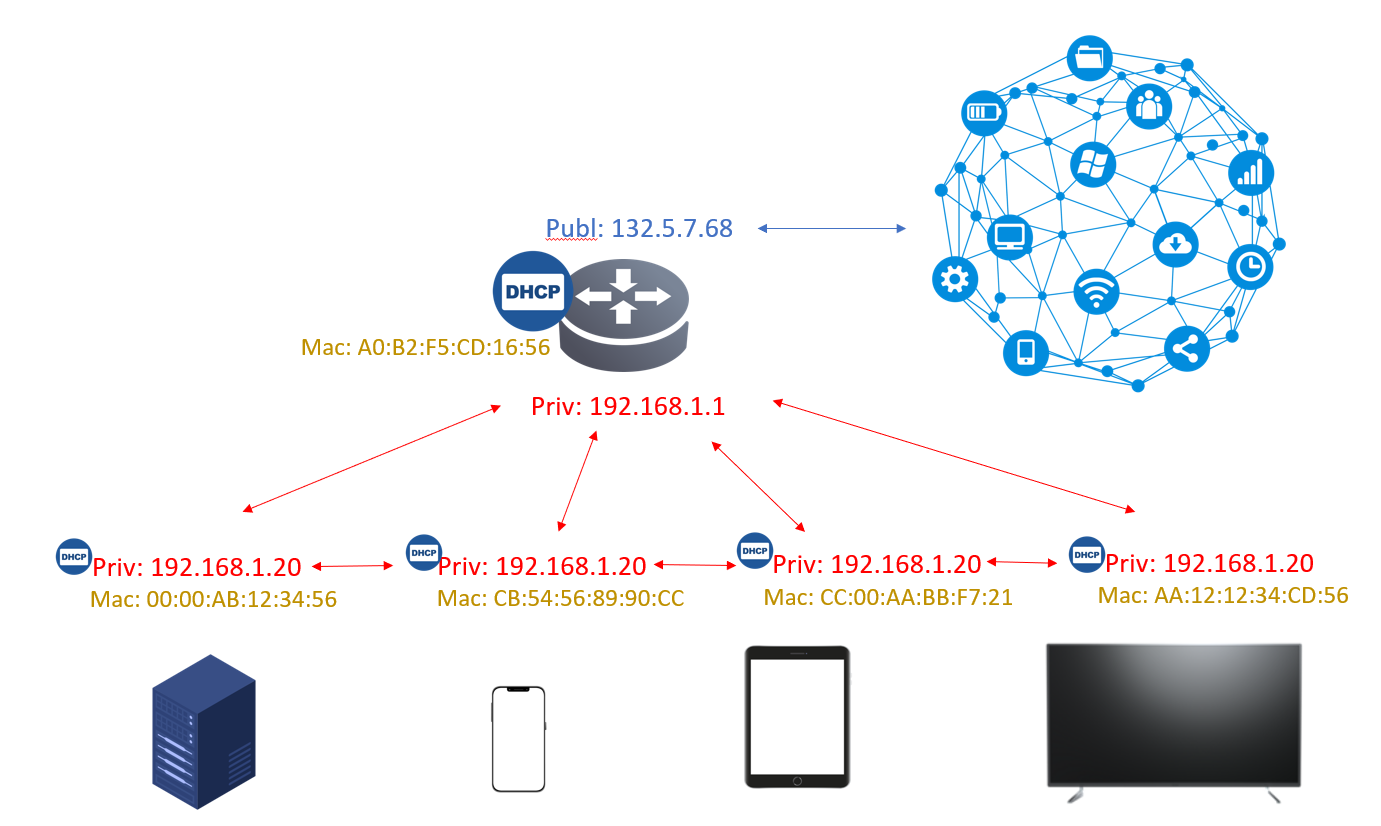
\includegraphics[width=\textwidth]{pictures/network.png}
    \centering
\end{figure}

\subsubsection{Advantages of have Private IP adresses}

\begin{itemize}
    \item \textbf{Address Space Conservation:} private IP addresses allow multiple devices to share a single public IP address (the one in the router), conserving the limited number of available public IP addresses.
    \item \textbf{Network Segmentation:} private IP addresses enable you to create a local network that can communicate internally without directly exposing each device to the internet.
    \item \textbf{Security:} : by using private IP addresses, devices within your local network are protected from direct access by external users on the internet.
\end{itemize}

\subsubsection{Can the private subnet be changed?}

Yes, you can change the subnet configuration of your router. This is useful if you have specific networking requirements or to avoid conflicts with other networks (e.g., when setting up a VPN or connecting to another network with the same default subnet).
\\\\
\textbf{How to Change It}
\begin{enumerate}
    \item \textbf{Access Router Settings:} open a web browser and enter the router's IP address (commonly 192.168.1.1 or 192.168.0.1) to access the router’s administration interface.
    \item \textbf{Login:} enter the admin username and password (default credentials are often found on the router or in the manual).
    \item \textbf{Navigate to Network Settings:} look for sections like "LAN Setup," "Network Configuration," or similar.
    \item \textbf{Change Subnet:} you can change the IP address range, such as changing from 192.168.1.0/24 to 192.168.2.0/24 or any other valid private IP range.
    \item \textbf{Save and Reboot:} save the changes and reboot the router for the new settings to take effect.
\end{enumerate}

\begin{blocktemplate}{NOTE}
You can change a lo of things in the router configuration following these instructions, the IP's assigned to some devices, static IP assignment instead of using DHCP, NAT rules, etc.
\end{blocktemplate}

\subsubsection{Private IP Address Ranges}

Private IP addresses are defined by the Internet Engineering Task Force (IETF) in RFC 1918. They are reserved for use within private networks and are not routable on the public internet. The commonly used private IP address ranges are:

\begin{itemize}
    \item 10.0.0.0 to 10.255.255.255
    \item 172.16.0.0 to 172.31.255.255
    \item 192.168.0.0 to 192.168.255.255
\end{itemize}

\subsubsection{Example of Private IP Assignment}
\begin{enumerate}
    \item \textbf{Router Configuration:} Your router might be configured to use the range 192.168.1.2 to 192.168.1.254 for DHCP.
    \item \textbf{Device Connection:} when your smartphone, laptop, tablet connects to the Wi-Fi, it sends a DHCP request asking for an IP address.
    \item Then the router's DHCP server assigns it 192.168.1.10 (for example) along with other network information.
\end{enumerate}



\subsection{FQDN} \label{FQDN}
El término Fully Qualified Domain Name (FQDN) se refiere a la dirección completa y única necesaria para tener presencia en Internet. Está compuesta por el nombre de host y el de dominio y se utiliza para localizar hosts específicos en Internet y acceder a ellos mediante la resolución de nombres. Este nombre de dominio único que contiene toda la información necesaria para poder acceder a una máquina a través de una red pública, como puede ser internet. A través de un FQDN un equipo es capaz de conectarse con cualquier otro.

La estructura del FQDN viene determinada por el sistema de nombres de dominio (DNS) y está conformada por etiquetas. Cada etiqueta se corresponde con el nombre de un nivel en el espacio de nombres de dominio y está separada de la siguiente por un punto. Ha de constar de entre 1 y 63 caracteres, que pueden ser números, letras y guiones (aunque realmente los guiones no se pueden usar al comenzar una etiqueta) y el total de caracteres del FQDN no debe exceder los 255. 

El Fully Qualified Domain Name consta como mínimo de tres etiquetas: el dominio de nivel superior, el nombre de dominio y el nombre de host. Se lee al revés.

\begin{figure}[H]
    \centering
    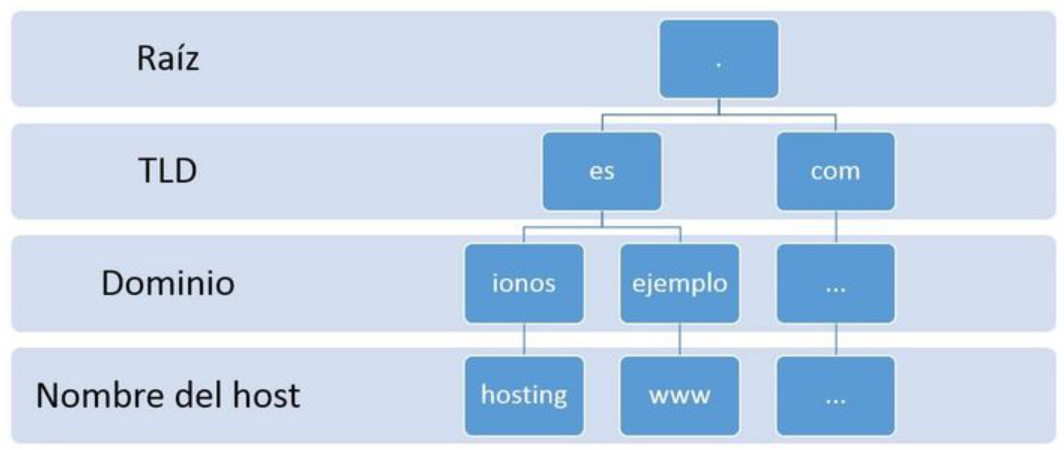
\includegraphics[scale=0.4]{pictures/image11.PNG}
    \label{FQDN Image}
    \caption{Representación esquemática de la estructura del Fully Qualified Domain Name}
\end{figure}

\textbf{Ejemplo de un FQDN}
\begin{verbatim}
[Nombre de host].[Dominio].[TLD]
\end{verbatim}
\begin{verbatim}
hosting.ionos.es
\end{verbatim}
\begin{enumerate}
    \item La etiqueta del dominio raíz tras el punto permanece vacía
    \item El \textbf{dominio de primer nivel:} en nuestro ejemplo es "\textit{.es}", dominio de nivel superior geográfico, también conocido por las siglas ccTLD (country code-top level domain). Frente a ellos se encuentran losTLD genéricos como .com o .org, también designados gTLD (generic top-level domain).
    \item El \textbf{dominio de segundo nivel}, también conocido como nombre de dominio.  En el ejemplo se corresponde con "\textit{ionos}".
    \item El \textbf{domino de tercer nivel}, en el extremo izquierdo, tenemos el nombre del host, en nuestro ejemplo "\textit{hosting}".
\end{enumerate}

Los FQDN se suelen utilizar en cualquier interacción en Internet, ya que son más fáciles de recordar que las direcciones IP. Otro ejemplo www.wordpress.com


Para más información consultad: \href{https://www.ionos.es/digitalguide/dominios/gestion-de-dominios/fully-qualified-domain-name/}{FQDN}
/ \href{https://www.hostinger.es/tutoriales/fqdn}{FQDN 2}

\subsection{DNS Resolution Process}

\subsubsection{Checking the Local Cache}
When you try to access an fqdn (like www.google.com), your machine first checks its local DNS cache to see if it already knows the IP address. This cache is typically managed by a service such as systemd-resolved, dnsmasq, or nscd.

\begin{figure}[H]
    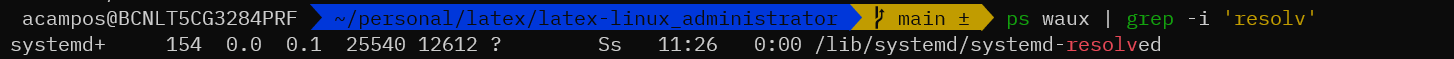
\includegraphics[width=\textwidth]{pictures/resolved.png}
    \centering
\end{figure}

\subsubsection{Hosts File}
If the address is not found in the cache, it then checks the \verb|/etc/hosts| file, which can have static mappings of hostnames to IP addresses.

\begin{codetemplate}{/etc/hosts}
\begin{verbatim}
127.0.0.1       localhost
8.8.8.8         www.dns-google.com
8.8.4.4         www.dns-google-2.com
9.9.9.9         quad9-dns.net
89.163.78.34    my.webpage.com
\end{verbatim}
\end{codetemplate}

\begin{blocktemplate}{Note}
In windows this file is in \verb|C:\Windows\System32\drivers\etc\hosts|
\end{blocktemplate}

\subsubsection{DNS Resolver Configuration}
If the fqdn is not found in the \verb+/etc/hosts+ file, the system uses DNS servers defined in the \verb+/etc/resolv.conf+ file. This file contains the IP addresses of the DNS servers that the system will query to resolve the domain name.

A typical \verb+/etc/resolv.conf+ might look like this:
\begin{codetemplate}{/etc/resolv.conf}
\begin{verbatim}
nameserver 9.9.9.9
nameserver 8.8.8.8
nameserver 8.8.4.4
\end{verbatim}
\end{codetemplate}

So the system sends a DNS query to one of the DNS servers listed in /etc/resolv.conf. The query asks for the IP address associated to the fqdn.
\begin{blocktemplateII}{Note}
The IP addresses 8.8.8.8, 8.8.4.4, and 9.9.9.9 are addresses for public DNS servers provided by different organizations. 8.8.8.8 and 8.8.4.4 are public DNS servers operated by Google. They are part of the Google Public DNS service, which was launched in December 2009. The service aims to make the web faster and more secure by providing a reliable and fast DNS resolution service.
\begin{itemize}
    \item 8.8.8.8: Primary DNS server
    \item 8.8.4.4: Secondary DNS server
\end{itemize}

9.9.9.9  is a public DNS server operated by Quad9, a nonprofit organization. Quad9 was launched in 2017 with the goal of improving internet security and privacy.

You also have the CloudFlare one in 1.1.1.1.
\end{blocktemplateII}

\subsubsection{Recursive DNS Resolution inside the DNS Server}
The DNS server might not know the answer immediately and may perform a recursive resolution process:

\begin{itemize}
    \item \textbf{Root DNS Servers:} The DNS server first contacts a root DNS server (one of the root name servers).
    \item \textbf{Top-Level Domain (TLD) Servers:} The root server responds with a referral to a TLD server (for .com domains, it would be a .com TLD server).
    \item \textbf{Authoritative DNS Servers:} The TLD server then provides a referral to the authoritative DNS server for google.com.
    \item \textbf{Final Resolution:} The authoritative DNS server for the fqdn responds with the IP address for the fqdn    
\end{itemize}

\subsubsection{Caching the Result}
Once the IP address is retrieved, it is sent back to your machine, which can now connect to the fqdn. This result is also cached locally to speed up future requests.

\subsection{DNS check Tools}

\subsubsection{nslookup}

nslookup (Name Server LOOKUP) is a network utility used for querying the Domain Name System (DNS) to obtain domain name or IP address mapping information. It is a command-line tool available on many operating systems, including Windows, macOS, and Linux. nslookup helps troubleshoot DNS-related issues by allowing users to query DNS servers and view the details of DNS records.

Basic usage
\begin{codetemplate}{}
\begin{verbatim}
$ nslookup example.com
\end{verbatim}
\end{codetemplate}

Specify a DNS Server to resolv the fqdn
\begin{codetemplate}{}
\begin{verbatim}
$ nslookup example.com 9.9.9.9
\end{verbatim}
\end{codetemplate}

Reverse Lookup: find the domain name associated with an IP address
\begin{codetemplate}{}
\begin{verbatim}
$ nslookup 8.8.4.4
\end{verbatim}
\end{codetemplate}

\subsubsection{dig}

dig (Domain Information Groper) is a network administration command-line tool for querying the Domain Name System (DNS). It is commonly used to retrieve information about DNS records, troubleshoot DNS issues, and verify DNS configurations. dig is widely used on Unix-like operating systems such as Linux and macOS, and it can also be installed on Windows.

Basic usage
\begin{codetemplate}{}
\begin{verbatim}
$ dig example.com
\end{verbatim}
\end{codetemplate}

Specify a DNS Server to resolv the fqdn
\begin{codetemplate}{}
\begin{verbatim}
$ dig @9.9.9.9 example.com
\end{verbatim}
\end{codetemplate}

Reverse Lookup: find the domain name associated with an IP address
\begin{codetemplate}{}
\begin{verbatim}
$ dig -x 8.8.4.4
\end{verbatim}
\end{codetemplate}

\textbf{Analysing the dig ouput}
\begin{itemize}
    \item \textbf{QUESTION SECTION:} The query you made.
    \item \textbf{ANSWER SECTION:} The resolved IP address(es) for www.google.com.
    \item \textbf{SERVER:} The DNS servers that are authoritative for the domain.
    \item \textbf{ADDITIONAL SECTION:} Any additional information provided by the DNS server.
\end{itemize}

Short answer
\begin{codetemplate}{}
\begin{verbatim}
$ dig +short example.com
\end{verbatim}
\end{codetemplate}

Verbose answer
\begin{codetemplate}{}
\begin{verbatim}
$ dig +trace example.com
\end{verbatim}
\end{codetemplate}

\subsection{Local Cache Services}

\subsubsection{systemd-resolved}

\verb+systemd-resolved+ is a system service provided by the systemd suite of system and service management tools for Linux operating systems. It is responsible for network name resolution, which means converting human-friendly domain names (like "example.com") into IP addresses that computers can use to communicate over a network. It is in charge of Caching and split DNS support for faster DNS resolution and optimized network usage.

The configuration files for \verb+systemd-resolved+:

\begin{itemize}
    \item \verb+/etc/systemd/resolved.conf+: Main configuration file for systemd-resolved. It contains settings for DNS servers, domains, and other options.
    \item \verb+/etc/resolv.conf+: typically, if you are using \verb+systemd-resolved+, it is a symbolic link pointing to    \verb+/run/systemd/resolve/resolv.conf+ or \verb+/run/systemd/resolve/stub-resolv.conf+. This file is what applications traditionally read to find DNS settings when they are not cached.
\end{itemize}

Check if \verb|systemd-resolved| is running
\begin{codetemplate}{}
\begin{verbatim}
$ ps waux | grep -i 'systemd-resolved'
\end{verbatim}
\end{codetemplate}
\begin{codetemplate}{}
\begin{verbatim}
$ sudo systemctl status systemd-resolved
\end{verbatim}
\end{codetemplate}

\subsubsection{dnsmasq}

dnsmasq is a lightweight, easy-to-configure DNS forwarder and DHCP server. It is designed to provide DNS, DHCP, TFTP, and PXE services for small networks. Here's a detailed look at dnsmasq:

Functions and features:

\begin{itemize}
    \item \textbf{DNS Forwarding:} forwards DNS queries to upstream DNS servers and caches the responses locally to speed up subsequent queries.
    \item \textbf{DNS Caching:} Caches DNS responses to improve performance and reduce load on upstream DNS servers.
    \item \textbf{DNS Masquerading:} Can provide custom DNS responses for local network addresses, which is useful for internal name resolution.
    \item \textbf{DHCP Server:} acts as a DHCP server, dynamically assigning IP addresses to devices on a local network. It supports DHCPv4 and DHCPv6.
    \item \textbf{TFTP Server:} provides Trivial File Transfer Protocol (TFTP) services, which are often used for network booting.
    \item \textbf{PXE Boot:} Supports network booting using PXE (Preboot Execution Environment), which is useful for diskless workstations or automated OS installations.
\end{itemize}

Main configuration file from \verb+dnsmasq+, it includes settings for DNS servers, DHCP ranges, TFTP options, and more: \verb|/etc/dnsmasq.conf|

Check if \verb|systemd-resolved| is running
\begin{codetemplate}{}
\begin{verbatim}
$ ps waux | grep -i 'dnsmasq'
\end{verbatim}
\end{codetemplate}
\begin{codetemplate}{}
\begin{verbatim}
$ sudo systemctl status dnsmasq
\end{verbatim}
\end{codetemplate}

\subsection{SSH}

\subsubsection{What is SSH?}

SSH, also known as Secure Shell or Secure Socket Shell, is a network protocol that gives users, particularly system administrators, a secure way to access a computer over an unsecured network.  Secure Shell provides strong password authentication and public key authentication, as well as encrypted data communications between two computers connecting over an open network, such as the internet.

In addition to providing strong encryption, SSH is widely used by network administrators to manage systems and applications remotely, enabling them to log in to another computer over a network, execute commands and move files from one computer to another.


The most basic use of SSH is to connect to a remote host for a terminal session. The form of that command is the following:
\begin{itemize}
    \item IP:
\begin{codetemplate}{}
\begin{verbatim}
$ ssh user_name@host_IP
\end{verbatim}
\end{codetemplate}
    \item Hostname:
\begin{codetemplate}{}
\begin{verbatim}
$ ssh user_name@SSHserve.example.com
\end{verbatim}
\end{codetemplate}   
\end{itemize}


The SSH key command instructs your system that you want to open an encrypted Secure Shell Connection. \verb|user_name| represents the account you want to access. For example, you may want to access the \verb|root| user or \verb|acampos| user.

\begin{blocktemplate}{Note}
To connect via ssh using a user, it is needed to have this user created in the host server.

\begin{itemize}
    \item \textbf{host server:} refers to the remote server you are trying to access.
    \item \textbf{client server:} refers to the server you are using to access the host.
\end{itemize}
\end{blocktemplate}

For the first time negotiating a connection between the client server and the host server, the user will be prompted with the remote host's public key fingerprint and prompted to connect.

\begin{codetemplate}{}
\begin{verbatim}
The authenticity of host 'sample.ssh.com' cannot be established.
 DSA key fingerprint is 01:23:45:67:89:ab:cd:ef:ff:fe:dc:ba:98:76:54:32:10.
 Are you sure you want to continue connecting (yes/no)?
\end{verbatim}
\end{codetemplate}

Answering yes to the prompt will cause the session to continue, and the host key is stored in the client server local system's \verb|known_hosts| file. This is a hidden file, stored by default in a hidden directory, called \verb|/.ssh/known_hosts|, in the user's home directory. Once the host key has been stored in the \verb|known_hosts| file, the client system can connect directly to that server again without need for any approvals; the host key authenticates the connection.

\begin{figure}[H]
    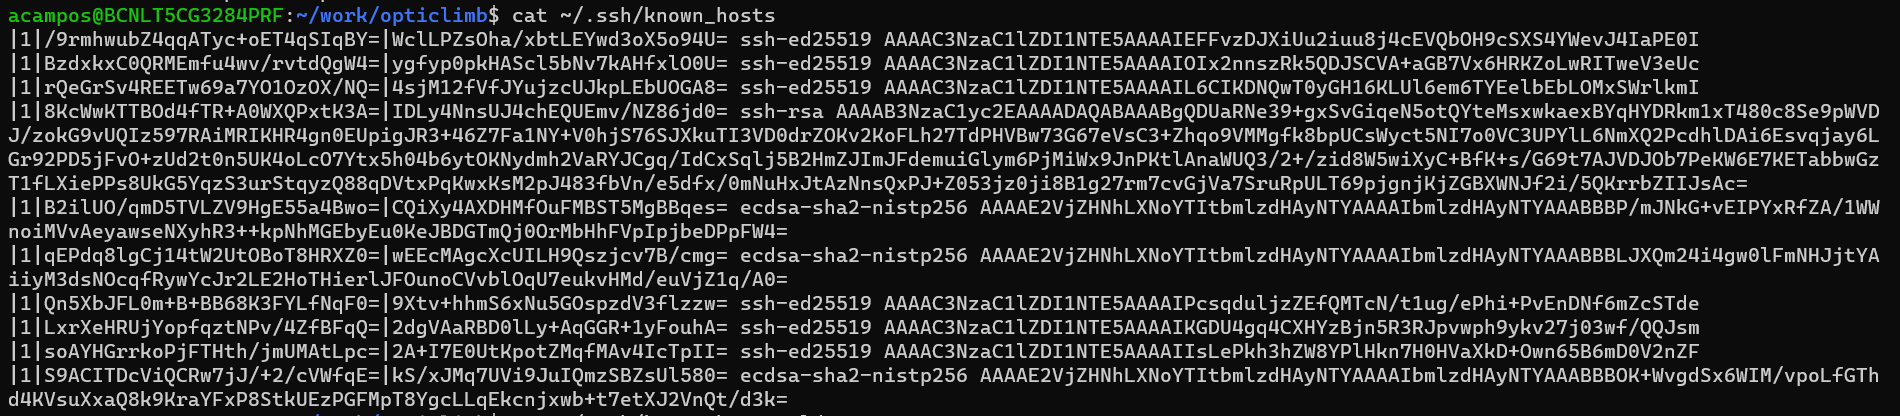
\includegraphics[width=\textwidth]{pictures/ssh1.png}
    \centering
\end{figure}

Present in all data centers, SSH ships by default with every Unix, Linux and Mac server. SSH connections have been used to secure many different types of communications between a local machine and a remote host, including secure remote access to resources, remote execution of commands, delivery of software patches, and updates and other administrative or management tasks, manage routers, server hardware, virtualization platforms, operating systems (OSes), and inside systems management and file transfer applications.

Secure Shell is used to connect to servers, make changes, perform uploads and exit, either using tools or directly through the terminal. SSH keys can be employed to automate access to servers and often are used in scripts, backup systems and configuration management tools.

\begin{blocktemplateI}{Note}

SSH operates on \textbf{TCP port 22} by default (though SSH port can be changed if needed). The host server listens on port 22 (or any other SSH assigned port) for incoming connections. It organizes the secure connection by authenticating the client and opening the correct shell environment if the verification is successful.
\\\\
It is hardly recommended to change the port in which the host server listen, because to let port 22 is more easily to enter the machine without authorization.
\end{blocktemplateI}

\subsubsection{Authenticate SSH connections using user-password}

By default SSH protocol doesn't use public key cryptography for authenticating hosts and users. It still uses the \textbf{Linux user-password authentication method}, so you only have to pass the \verb|username| of the Linux user via the ssh command and introduce the \verb|password| of this user:

\begin{codetemplate}{}
\begin{verbatim}
$ ssh -p custom_port linux_username@hostname_or_ip
\end{verbatim}
\end{codetemplate}

\begin{blocktemplate}{Note}
 If you run the command without specifying user, ssh will take the client server Linux current \verb|username|.
\end{blocktemplate}

\subsubsection{Authenticate SSH connections using Asimetric Key authentication method}

Generally, the SSH service is configured to use Asimetric Key cryptography for authenticating hosts and users. SSH introduced Asimetric Key authentication as a more secure alternative to the older \verb|.rhosts| authentication. It improved security by avoiding the need to have password stored in files, and eliminated the possibility of a compromised server stealing the user's password.

However, SSH keys are authentication credentials just like passwords. Thus, they must be managed somewhat analogously to user names and passwords. They should have a proper termination process so that keys are removed when no longer needed.

\paragraph{Generate public and private keys on the client server side}

For that reason, we should generate SSH public and private key on our client and authorize them into the host.

Depending on the technology of the host you want to connect, you need to create the keys:

\begin{itemize}
    \item \textbf{rsa:} an old algorithm based on the difficulty of factoring large numbers. A key size of at least 2048 bits is recommended for RSA; 4096 bits is better. All SSH clients support this algorithm.
\begin{codetemplate}{}
\begin{verbatim}
$ ssh-keygen -t rsa -b 4096 -f ~/.ssh/key_name -C "your_email@example.com" 
\end{verbatim}
\end{codetemplate}
    \item \textbf{ed25519:} this is a new algorithm added in OpenSSH. Support for it in clients is not yet universal.
\begin{codetemplate}{}
\begin{verbatim}
$ ssh-keygen -t ed25519 -f ~/.ssh/key_name -C "your_email@example.com"
\end{verbatim}
\end{codetemplate}
\end{itemize}

\begin{blocktemplateI}{Note}
Main differences between RSA and Ed25519:
\begin{itemize}
    \item \textbf{Algorithm Type:} RSA is based on the difficulty of factoring large numbers, while Ed25519 uses elliptic curve cryptography.
    \item \textbf{Key Size:} RSA typically uses 2048 or 4096-bit keys; Ed25519 uses a fixed 256-bit key.
    \item \textbf{Security Level:} Ed25519 offers similar security to a 3072-bit RSA key with a smaller key size.
    \item \textbf{Performance:} Ed25519 is much faster in signing, verification, and key generation compared to RSA.
    \item \textbf{Adoption:} RSA is widely adopted and compatible with many systems; Ed25519 is gaining popularity, especially in modern protocols.
    \item \textbf{Use Cases:} RSA is common in SSL/TLS and email encryption, while Ed25519 is favored in SSH, DNSSEC, and other performance-critical applications.
\end{itemize}
\end{blocktemplateI}

They will ask your for passphrase, depending on your security needs you can put one or not. If you introduce one, it will ask for them each time the keys are used.

\begin{blocktemplateIII}{WARNING}
For SSH to recognize the SSH keys they should be stored in:
\begin{codetemplate}{}
\begin{verbatim}
~/.ssh/
\end{verbatim}
\end{codetemplate}
\begin{figure}[H]
    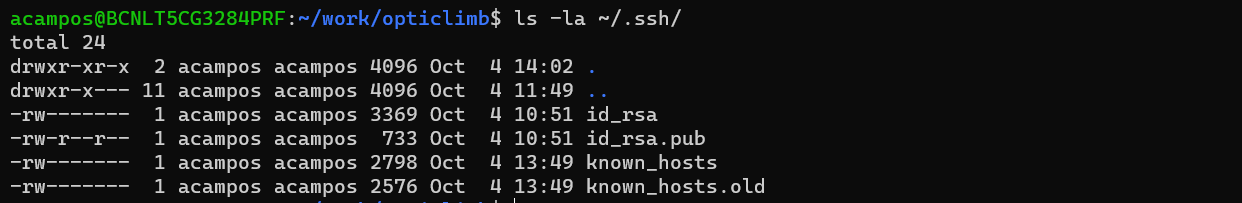
\includegraphics[width=\textwidth]{pictures/ssh2.png}
    \centering
\end{figure}
Also, \textbf{rsa keys} should have the \textbf{permissions} you see in the image above, if not, it will not be valid to authenticate in any server. If you have generated the keys, they are generated with the correct permissions, but if you have copied, it can be wrong.
\end{blocktemplateIII}

\begin{blocktemplateII}{Note}
If you have multiple rsa keys, it is hardly recommended to create a \verb+known_hosts+ file for each account you have because it makes diagnosing issues easier when you have multiple keys. Ideally the name of this file is similar enough to the key name that you aren't confused later.

\begin{codetemplate}{}
\begin{verbatim}
$ touch known_hosts_keyname
\end{verbatim}
\end{codetemplate}
\end{blocktemplateII}

For more information, check the documentation of \href{https://docs.github.com/en/authentication/connecting-to-github-with-ssh/generating-a-new-ssh-key-and-adding-it-to-the-ssh-agent}{how to do if for github servers}.

\paragraph{Optional - Set up the ssh config file}

The \verb+~/.ssh/config+ can contain specific configuration for each host. For example:

\begin{codetemplate}{~/.ssh/config}
\begin{verbatim}
# Github
Host github.com
  Hostname github.com
  User git
  AddKeysToAgent yes
  UseKeychain yes
  IdentityFile ~/.ssh/github_key
  UserKnownHostsFile ~/.ssh/konwn_hosts_github
  IdentitiesOnly yes

# Bitbucket
Host bitbucket.org
  HostName bitbucket.org
  User git
  AddKeysToAgent yes
  UseKeychain yes
  IdentityFile ~/.ssh/bitbucket_key
  UserKnownHostsFiles ~/.ssh/known_hosts_bitbucket
  IdentitiesOnly yes
\end{verbatim}
\end{codetemplate}

Here is the breakdown of what each line means:

\begin{itemize}
    \item \textbf{Host} is a pattern matcher that is used to differentiate between these sets of configurations. Keep it the same as the HostName so it matches hosts in connections correctly without additional specification.
    \item Host The URL on the \textbf{HostName} line is the base URL where the repository resides. For example, if you have a personal account on github with personal projects, the URL will be github.com.
    \item \textbf{User} for git based systems will be git. The value of User will be different if you connect to something else (i.e. ec2-user for connecting to an Amazon AWS EC2 instance)
    \item \textbf{IdentityFile} asks for the location of the identity key we made. Type in the respective path here.
    \item \textbf{AddKeysToAgent} allows a private key that is used during authentication to be added to ssh-agent if it is running
    \item \textbf{UseKeychain} (macOS only) allows the computer to remember the password each time it restarts
    \item \textbf{UserKnownHostsFile} specifies an exact location to store all hosts you connect to when you're using that profile. Provide the respective paths here and choose a unique known hosts file name (see step 2 above) so that troubleshooting and key maintenance over time is easier.
    \item \textbf{IdentitiesOnly} specifies that only the keys provided must be used to connect to a host, even if another service like the ssh-agent offers a key for use.
\end{itemize}




\paragraph{Upload the Public Key into the authorized\_keys of the host server}
To use public key authentication, the public key must be \textbf{installed in the} \verb|authorized_keys| file of the server. This can be conveniently done using the \verb|ssh-copy-id tool|. Like this:

\begin{codetemplate}{}
\begin{verbatim}
$ ssh-copy-id -i ~/.ssh/my_ssh_key.pub user_name@hostname
\end{verbatim}
\end{codetemplate}

\begin{blocktemplateIII}{WARNING}
With the command above, we will append the host \textbf{pubkey} in the \verb|authorized_keys| file of the server.
\end{blocktemplateIII}

The authorized keys to enable an specific user accessing the server through ssh are stored in:

\begin{codetemplate}{}
\begin{verbatim}
~/.ssh/authorized_keys
\end{verbatim}
\end{codetemplate}
    
So you can copy your public key directly to this directory inside the server.

\begin{blocktemplateII}{Note}
For git you should do it different, just adding your public ssh key in the GUI, accessing to your profile settings. You can follow the \href{https://docs.github.com/en/authentication/connecting-to-github-with-ssh/adding-a-new-ssh-key-to-your-github-account}{Official Documentation}
\end{blocktemplateII}

\paragraph{Configure the ssh service into the host server}

To enable the SSH connection, the host server we want to connect should have the ssh service running and configured. 

We can check if the sshd (ssh daemon) service is running. SSH Daemon listens for incoming SSH connections and handles authentication, encryption, and communications: 

\begin{codetemplate}{}
\begin{verbatim}
$ systemctl status sshd
\end{verbatim}
\end{codetemplate}

\begin{blocktemplateIII}{WARNING}
So not confuse it with the ssh service,  which is the one used on the client-side to establish a secure connection to an SSH server. 
\end{blocktemplateIII}

The configuration file for the SSH Daemon is:
\begin{codetemplate}{}
\begin{verbatim}
/etc/ssh/sshd_config
\end{verbatim}
\end{codetemplate}

As we said before, by default SSH protocol doesn't use public key cryptography for authenticating hosts and users. So to enable it, we will need to modify this file in order to decoment the line:
\begin{codetemplate}{/etc/ssh/sshd\_config}
\begin{verbatim}
PubkeyAuthentication yes
\end{verbatim}
\end{codetemplate}

And then restart the sshd service:
\begin{codetemplate}{}
\begin{verbatim}
$ systemctl restart sshd
\end{verbatim}
\end{codetemplate}

\begin{blocktemplateII}{NOTE}
As well you can disable the password authentication:
\begin{codetemplate}{/etc/ssh/sshd\_config}
\begin{verbatim}
PasswordAuthentication no
\end{verbatim}
\end{codetemplate}
\end{blocktemplateII}

To see all the configurable parameters in the \verb|/etc/ssh/sshd_config| you can check

\begin{itemize}
    \item \href{https://www.ssh.com/academy/ssh/sshd_config}{All configurable parameters in sshd file}
    \item Your template in ansible
\end{itemize}


\paragraph{Use the Asimetric Key authentication method using -i}

By default, when you try to stablish ssh connection, if the host server enables PubkeyAuthentication, your ssh service will try to authenticate with all this pub keys:
\begin{itemize}
    \item \verb|~/.ssh/id_ecdsa.pub|
    \item \verb|~/.ssh/id_ecdsa_sk.pub|
    \item \verb|~/.ssh/id_ed25519.pub|
    \item \verb|~/.ssh/id_ed25519_sk.pub|
    \item \verb|~/.ssh/id_xmss.pub|
    \item \verb|~/.ssh/id_xmss_sk.pub|
    \item \verb|~/.ssh/id_dsa.pub|
    \item \verb|~/.ssh/id_rsa.pub|
\end{itemize}

If you want to enforce the client server ssh service use just one, or a custom one different from those shown, you should:
\begin{codetemplate}{}
\begin{verbatim}
$ ssh -p <Port_Number> -i /path/to/the/priv_key
\end{verbatim}
\end{codetemplate}

\begin{blocktemplate}{NOTE}
You should have both keys on the same folder, public and private, if not, it will fail.
\end{blocktemplate}

\paragraph{Use the ssh-agent for Asimetric Key}

SSH agent is program which runs in the background and stores your decrypted private keys for SSH authentication. It helps you manage your SSH keys securely without having to enter their passphrase every time you use them. It is very useful as well when your keys have passphrase.

So in order to use to store your ssh private keys you should:

\begin{enumerate}
    \item Check if it is running (it is not enabled when Boot by default so if you dont do it manually when boot the terminal it won't be running)
\begin{codetemplate}{}
\begin{verbatim}
$ ps waux | grep -e "ssh-agent"
\end{verbatim}
\end{codetemplate}

    \item If it is not running (you dont have any process with ssh-agent), initiate it:
\begin{codetemplate}{}
\begin{verbatim}
$ eval "$(ssh-agent -s)"
\end{verbatim}
\end{codetemplate}

    \item Add your private keys to the agent
\begin{codetemplate}{}
\begin{verbatim}
$ ssh-add /path/to/the/priv/key
\end{verbatim}
\end{codetemplate}

    \item Run your ssh normally (without specifing private key -i)
\end{enumerate}

\subsubsection{SSH Extra Arguments}

\textbf{Custom Port (by default is 22)}
\begin{codetemplate}{}
\begin{verbatim}
$ ssh -p <Port_Number>
\end{verbatim}
\end{codetemplate}

\textbf{Use specific pub\_key to authenticate}
\begin{codetemplate}{}
\begin{verbatim}
$ ssh -i /path/to/the/priv_key ...
\end{verbatim}
\end{codetemplate}

\textbf{Disable Check on the hosts file for this host}
\begin{codetemplate}{}
\begin{verbatim}
$ ssh -o StrictHostKeyChecking=no ...
\end{verbatim}
\end{codetemplate}

\textbf{Verbose Mode}
\begin{codetemplate}{}
\begin{verbatim}
$ ssh -v ...
\end{verbatim}
\end{codetemplate}

\textbf{Set timeout}
\begin{codetemplate}{}
\begin{verbatim}
$ ssh -o ConnectTimeout=30 ...
\end{verbatim}
\end{codetemplate}

\textbf{Using Proxy to establish the connection}
\begin{codetemplate}{}
\begin{verbatim}
$ ssh -o ProxyCommand="ssh -p <Proxy_Port_Number> -W %h:%p \
    -q <username>@<proxy_hostname_or_ip>"
\end{verbatim}
\end{codetemplate}

\subsubsection{SFTP}

\subsubsection{Introduction}
FTP, or "File Transfer Protocol" was a popular unencrypted method of trans-
ferring files between two remote systems.

SFTP, which stands for SSH File Transfer Protocol, or Secure File Transfer
Protocol, is a separate protocol packaged with SSH that works in a similar way
but over a secure connection. The advantage is the ability to leverage a secure
connection to transfer files and traverse the filesystem on both the local and
remote system.

In almost all cases, SFTP is preferable to FTP because of its underlying security
features and ability to piggy-back on an SSH connection. FTP is an insecure
protocol that should only be used in limited cases or on networks you trust.

\textbf{Basic Usage}
\begin{codetemplate}{}
\begin{verbatim}
$ sftp -P <Port_Number> <username>@<hostname_or_ip>
\end{verbatim}
\end{codetemplate}

\textbf{Set timeout}
\begin{codetemplate}{}
\begin{verbatim}
$ sftp -o ConnectTimeout=30 ...
\end{verbatim}
\end{codetemplate}

You will be asked to insert the password if the sshd service is configured with password, so there is a way to insert it wihout be asked.

\textbf{Send te password without interaction}
\begin{codetemplate}{}
\begin{verbatim}
$ sshpass -p "your_password" sftp -P ...
\end{verbatim}
\end{codetemplate}

\subsubsection{Commands inside the SFTP}

Once you are inside the sftp you can execute the follogin commands:

\paragraph{Navigate}

\textbf{Ask for help}
\begin{codetemplate}{}
\begin{verbatim}
sftp> help
\end{verbatim}
\end{codetemplate}

\textbf{Navigate through directories}
\begin{codetemplate}{}
\begin{verbatim}
sftp> pwd
\end{verbatim}
\end{codetemplate}

\begin{codetemplate}{}
\begin{verbatim}
sftp> ls -la
\end{verbatim}
\end{codetemplate}

\begin{codetemplate}{}
\begin{verbatim}
sftp> cd /the/path/you/want
\end{verbatim}
\end{codetemplate}

Create a directory
\begin{codetemplate}{}
\begin{verbatim}
sftp> mkdir folder
\end{verbatim}
\end{codetemplate}

\begin{blocktemplateI}{NOTE}
You wont be able to remove it from sftp, you need to access the server via ssh and remove it
\end{blocktemplateI}

\textbf{Displays a folder/file disk space usage inside host server}
\begin{codetemplate}{}
\begin{verbatim}
sftp> df -h folder_name
\end{verbatim}
\end{codetemplate}

\textbf{Execute commands in your local machine (client server)}

If you include "!" before your command, you will execute this command on your local linux machine
\begin{codetemplate}{}
\begin{verbatim}
sftp> !ls
\end{verbatim}
\end{codetemplate}

\paragraph{Get}

\textbf{Get file from host server to client server}
\begin{codetemplate}{}
\begin{verbatim}
sftp> get /path/to/the/remote/file /path/to/the/local/file
\end{verbatim}
\end{codetemplate}

\textbf{Get directory from host server to client server}
\begin{codetemplate}{}
\begin{verbatim}
sftp> get -Pr /path/to/the/remote/directory /path/to/the/local/directory
\end{verbatim}
\end{codetemplate}

\begin{blocktemplateI}{NOTE}
The \verb|-P| is to maintain the appropriate permissions and access times
\end{blocktemplateI}

\paragraph{Put}

\textbf{Upload client server file to host server}
\begin{codetemplate}{}
\begin{verbatim}
sftp> put /path/to/the/local/file /path/to/the/remote/file
\end{verbatim}
\end{codetemplate}

\textbf{Upload directory from cliient server to host server}
\begin{codetemplate}{}
\begin{verbatim}
sftp> put -Pr /path/to/the/local/directory /path/to/the/remote/directory
\end{verbatim}
\end{codetemplate}

\begin{blocktemplateI}{NOTE}
The \verb|-P| is to maintain the appropriate permissions and access times
\end{blocktemplateI}

\paragraph{Exit}
\begin{codetemplate}{}
\begin{verbatim}
sftp> bye
\end{verbatim}
\end{codetemplate}

\begin{codetemplate}{}
\begin{verbatim}
sftp> exit
\end{verbatim}
\end{codetemplate}

\begin{codetemplate}{}
\begin{verbatim}
sftp> !
\end{verbatim}
\end{codetemplate}

\subsubsection{Being sudo with SFTP?}


In general, the sudo command is not directly applicable to SFTP (SSH File Transfer Protocol) because SFTP is a protocol specifically designed for transferring files securely over SSH (Secure Shell). However, if you want to perform administrative tasks on a remote server using SFTP, you typically need to have the appropriate permissions granted to your SSH user account.

If you need to perform administrative tasks on files through SFTP, you would typically ensure that the user account you're logging in with has the necessary permissions to read, write, and modify those files. 

\begin{codetemplate}{}
\begin{verbatim}
$ ssh ... username@remote_server
\end{verbatim}
\end{codetemplate}

\begin{codetemplate}{}
\begin{verbatim}
$ sudo command_to_execute
\end{verbatim}
\end{codetemplate}

\begin{codetemplate}{}
\begin{verbatim}
$ sftp ... username@remote_server
\end{verbatim}
\end{codetemplate}

\subsection{Localhost Networking}
\subsubsection{Ports Exposed}

Para saber que puertos tiene escuchando nuestro localhost:

\begin{enumerate}
    \item Using \verb|lsoft|
\begin{codetemplate}{}
\begin{verbatim}
$ sudo lsof -i -P -n
\end{verbatim}
\end{codetemplate}
\begin{codetemplate}{}
\begin{verbatim}
$ sudo lsof -i -P -n | grep -i listen
\end{verbatim}
\end{codetemplate}

    \item Using \verb|netstat|
\begin{codetemplate}{}
\begin{verbatim}
$ netstat -putona | grep numero-de-puerto
\end{verbatim}
\end{codetemplate}

\begin{itemize}
    \item \textbf{p:} muestra las conexiones para el protocolo especificado que puede ser TCP o UDP
    \item \textbf{u:} lista todos los puertos UDP
    \item \textbf{t:} lista todos los puertos TCP
    \item \textbf{o:} muestra los timers
    \item \textbf{n:} muestra el numero de puerto
    \item \textbf{a:} visualiza todas las conexiones activas del sistema
\end{itemize}
\end{enumerate}

\begin{blocktemplate}{NOTE}
\verb|netstat| command shows the system’s network information, like routing and sockets.
\end{blocktemplate}

\subsubsection{Localhost Adresses}

\textbf{De puertas para adentro}
\begin{enumerate}
    \item \textbf{Ipv4:}
    \begin{itemize}
        \item localhost
        \item 127.0.0.1
    \end{itemize}
    \item \textbf{Ipv6}
    \begin{itemize}
        \item 0:0:0:0:0:0:0:1
        \item ::1
    \end{itemize}
\end{enumerate}

\textbf{De puertas para fuera}
\begin{itemize}
    \item \verb|ifconfig|: displays the system’s network interfaces and their configurations. In this case our localhost direction to outside is 172.21.220.125/20 (172.21.220.125 with mask 255.255.240.0)
\begin{codetemplate}{}
\begin{verbatim}
$ ifconfig
\end{verbatim}
\end{codetemplate}
\begin{figure}[H]
    \centering
    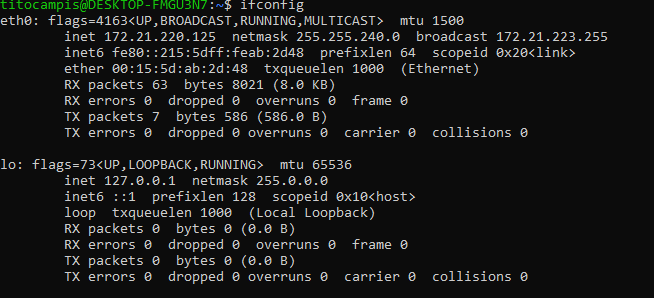
\includegraphics[scale=0.45]{pictures/image35.PNG}
    \caption{ifconfig}
\end{figure}
    
    \item \verb|ip -br addr list eth0|
    \begin{figure}[H]
    \centering
    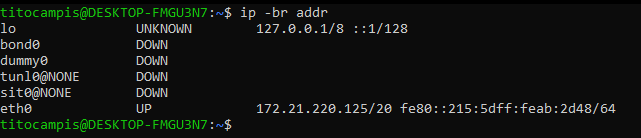
\includegraphics[scale=0.45]{pictures/image36.PNG}
    \caption{ip -br}
\end{figure}
\end{itemize}

\begin{blocktemplateIII}{Nota}
\begin{codetemplate}{Netmask}
\begin{verbatim}
24 (number of 1's):
255.255.255.0
11111111 11111111 11111111 00000000

20 (number of 1's):
255.255.240.0
11111111 11111111 11110000
\end{verbatim}
\end{codetemplate}
\end{blocktemplateIII}

\subsection{Certificates}


\newpage
%-------------------------------------------------------------------------------------------------
\section{Network Tools}

\subsection{Ping}

Ping is a network utility used to test the reachability of a host on an Internet Protocol (IP) network and measure the round-trip time for packets sent from the source to the destination host and back. It works by sending Internet Control Message Protocol (ICMP) echo request packets to the target host and waiting for ICMP echo reply packets in response.

\textbf{Basic Usage}
\begin{codetemplate}{}
\begin{verbatim}
$ ping <hostname_or_ip>
\end{verbatim}
\end{codetemplate}

\textbf{Sned specific number of packages}
\begin{codetemplate}{}
\begin{verbatim}
$ ping -c <number_of_packages> ...
\end{verbatim}
\end{codetemplate}

\textbf{Set interval between sending ping requests in seconds}
\begin{codetemplate}{}
\begin{verbatim}
$ ping -i <interval_seconds> ...
\end{verbatim}
\end{codetemplate}

\textbf{Set timeout for packages}
\begin{codetemplate}{}
\begin{verbatim}
$ ping -t <timeout_seconds> ...
\end{verbatim}
\end{codetemplate}

\textbf{Set timeout for ping (deadline in seconds)}
\begin{codetemplate}{}
\begin{verbatim}
$ ping -W <timeout_seconds> ...
\end{verbatim}
\end{codetemplate}

\textbf{Stopping ping}
\begin{codetemplate}{}
\begin{verbatim}
$ Ctrl+C
\end{verbatim}
\end{codetemplate}

\begin{blocktemplateIII}{WARNING}
Use ping to "ping" an IP address doesn't necessarily mean that you can access services like SSH, HTTP, database, HTTPS, or others on that IP. Ping operates at the ICMP (Internet Control Message Protocol) level, which is a lower level than the protocols used by services like SSH (Secure Shell), HTTP or database (TCP), HTTPS (HTTP over SSL/TLS), or others.
\\\\
So ping is not a good method to check the connection to an specific service running on a host. You can use it to check if you can resolve / reach a host, but not to check if you can reach a database inside this host. Because the network and firewall rules are usually deffined by protocol, they use to allow ICMP echo requests (which is what ping uses) for diagnostic purposes, but blocks other types of traffic such as SSH, TCP, HTTP, HTTPS... for security reasons. 
\end{blocktemplateIII}

\subsection{Curl}

Curl (Client for URL's) is a command-line tool and library for transferring data with URLs. It is mainly intended for testing HTTP and HTTPS connections, but it supports various protocols more: FTP, FTPS, SCP, SFTP, LDAP, TELNET, and more. 

Curl is widely used for testing web services, downloading / uploading files, and automating data transfers in scripts and applications. 

It is a powerful tool for accessing and transferring data over networks, with support for multiple protocols and versatile capabilities. But for network connectivity, it is not so suitable tool, because there are many protocols not supported by curl. 

It can happen that with curl we get a connection error and it is not because the connection itself is not open, but because we are not using the correct protocol.

\textbf{Basic Usage}
\begin{codetemplate}{}
\begin{verbatim}
$ curl <url> 
\end{verbatim}
\end{codetemplate}

\textbf{Using proxy}
\begin{codetemplate}{}
\begin{verbatim}
$ curl -x <proxy_url> <url> 
\end{verbatim}
\end{codetemplate}

\textbf{Forcing no proxy}
\begin{codetemplate}{}
\begin{verbatim}
$ curl --noproxy "*" <url>
\end{verbatim}
\end{codetemplate}


\textbf{With specific timeout in seconds}
\begin{codetemplate}{}
\begin{verbatim}
$ curl --connect-timeout 5 ...
\end{verbatim}
\end{codetemplate}

\textbf{Not show content, only info}
\begin{codetemplate}{}
\begin{verbatim}
$ curl -I ...
\end{verbatim}
\end{codetemplate}

\textbf{Follow redirects}

To have more context, when you make an HTTP request to a server, it might respond with a redirect status code (such as 301 Moved Permanently or 302 Found) along with the new URL to which the request should be redirected. By default, tools like curl won't automatically follow these redirects; instead, they'll stop and return the redirect response to the user.

When you use the -L option with curl, it instructs curl to follow HTTP redirects automatically. So, when curl encounters a redirect response (e.g., a 301 or 302 status code), it will automatically make a new request to the URL specified in the redirect response.

\begin{codetemplate}{}
\begin{verbatim}
$ curl -L ...
\end{verbatim}
\end{codetemplate}

\textbf{Force the protocol}
\begin{codetemplate}{}
\begin{verbatim}
$ -0,       --http1.0            Use HTTP 1.0
            --http1.1            Use HTTP 1.1
            --http2              Use HTTP 2
            --http2-prior-knowledge Use HTTP 2 without HTTP/1.1 Upgrade
            --http3              Use HTTP v3
\end{verbatim}
\end{codetemplate}

\textbf{Download a file via https}
\begin{codetemplate}{}
\begin{verbatim}
$ curl -O https://url/paht/to/file
\end{verbatim}
\end{codetemplate}

\textbf{Download a file to specific path}
\begin{codetemplate}{}
\begin{verbatim}
$ curl -o /path/to/the/filename https://url/paht/to/file
\end{verbatim}
\end{codetemplate}

\textbf{Upload a file using https protocol}
\begin{codetemplate}{}
\begin{verbatim}
$ curl -F "file=@/path/to/local/file.txt" https://example.com/upload
\end{verbatim}
\end{codetemplate}

\textbf{Upload a file using ftp protocol}
\begin{codetemplate}{}
\begin{verbatim}
$ curl -T /path/to/local/file.txt ftp://ftp.example.com/upload/
\end{verbatim}
\end{codetemplate}

\textbf{Target different port than 443 or 8080}
\begin{codetemplate}{}
\begin{verbatim}
$ curl domain:port
\end{verbatim}
\end{codetemplate}

\textbf{Verbose}
\begin{codetemplate}{}
\begin{verbatim}
$ curl -v 
\end{verbatim}
\end{codetemplate}

\textbf{HTTPS Protocol (port 443)}
\begin{codetemplate}{}
\begin{verbatim}
$ curl https://hostname
\end{verbatim}
\end{codetemplate}
\begin{codetemplate}{}
\begin{verbatim}
$ curl hostname:443
\end{verbatim}
\end{codetemplate}

\textbf{Allow insecure connections, skip certificate validation}
\begin{codetemplate}{}
\begin{verbatim}
$ curl -k hostname
\end{verbatim}
\end{codetemplate}

\textbf{Authentication}
\begin{codetemplate}{}
\begin{verbatim}
$ curl -u user_name:pwd hostname 
\end{verbatim}
\end{codetemplate}

\textbf{Pass Headers}
\begin{codetemplate}{}
\begin{verbatim}
$ curl -H "Content-Type:application/json" hostname 
\end{verbatim}
\end{codetemplate}

\textbf{GET HTTP Requests}
\begin{codetemplate}{}
\begin{verbatim}
$ curl -XGET -H hostname 
\end{verbatim}
\end{codetemplate}

\textbf{PUT HTTP Requests}
\begin{codetemplate}{}
\begin{verbatim}
$ curl -XPUT hostname 
\end{verbatim}
\end{codetemplate}

\textbf{POST HTTP Requests}
\begin{codetemplate}{}
\begin{verbatim}
$ curl -XPOST hostname 
\end{verbatim}
\end{codetemplate}

\textbf{POST HTTP Requests}
\begin{codetemplate}{}
\begin{verbatim}
$ curl -XDELETE hostname 
\end{verbatim}
\end{codetemplate}

\subsection{Nmap}

Nmap, short for Network Mapper, is a powerful open-source tool primarily used for network discovery and security auditing. It's designed to provide a comprehensive overview of the devices and services running on a network.

It helps in identifying hosts, devices, and services running on a network. It provides essential information such as IP addresses, MAC addresses, and open ports. One of its core functionalities is port scanning, which involves probing a target host to determine which ports are open, closed, or filtered. This information is crucial for understanding the network's security posture and potential vulnerabilities.

Nmap can detect the version and type of services running on open ports. This capability allows administrators to assess the software stack of networked devices and identify outdated or vulnerable services. Nmap can often determine the operating system (OS) running on a target host based on subtle differences in network stack implementations and responses to specific probes. This feature aids in network mapping and security assessment.

\textbf{Basic TCP port scan on a specific host}
\begin{codetemplate}{}
\begin{verbatim}
$ nmap <hostname_or_ip>
\end{verbatim}
\end{codetemplate}

\textbf{Discover a host on a network}
\begin{codetemplate}{}
\begin{verbatim}
$ nmap -sn <hostname_or_ip>
\end{verbatim}
\end{codetemplate}

\textbf{Scan specific ports}
\begin{codetemplate}{}
\begin{verbatim}
$ nmap -p <port_name> <hostname_or_ip>
\end{verbatim}
\end{codetemplate}
\begin{codetemplate}{}
\begin{verbatim}
$ nmap -p 80,443,... <hostname_or_ip>
\end{verbatim}
\end{codetemplate}

\textbf{Scan range of ports}
\begin{codetemplate}{}
\begin{verbatim}
$ nmap -p 80-443 <hostname_or_ip>
\end{verbatim}
\end{codetemplate}

\textbf{Scan all ports}
\begin{codetemplate}{}
\begin{verbatim}
$ nmap -p- <hostname_or_ip>
\end{verbatim}
\end{codetemplate}

\textbf{Scan the 100 more used ports}
\begin{codetemplate}{}
\begin{verbatim}
$ nmap -F <hostname_or_ip>
\end{verbatim}
\end{codetemplate}

\textbf{Detect the operating system of the target host}
\begin{codetemplate}{}
\begin{verbatim}
$ nmap -O <hostname_or_ip>
\end{verbatim}
\end{codetemplate}

\textbf{Do not check using ping if the host is up, just try the connection to ports}

It is really useful when the host blocking our pings
\begin{codetemplate}{}
\begin{verbatim}
$ nmap -Pn <hostname_or_ip>
\end{verbatim}
\end{codetemplate}

\textbf{Scan all the ports opened of the target host}
\begin{codetemplate}{}
\begin{verbatim}
$ nmap -sT -T Aggressive <hostname_or_ip>
\end{verbatim}
\end{codetemplate}

\begin{blocktemplateII}{NOTE}
The services shown in the output of nmap are not exact, it is what is commonly exposed on the port, but it cannot know what is exactly exposed on the ports.
\end{blocktemplateII}

\subsection{Netcat}

Netcat, often referred to as the "Swiss Army Knife" of networking tools, is a versatile utility for reading from and writing to network connections using TCP/IP protocols. It can act both as a client and a server. It can establish connections, listen for connections, and transfer data in various ways.

\textbf{Check if a port is open on a remote server}
\begin{codetemplate}
\begin{verbatim}
$ nc -zv <hostname_or_ip> <port_number>
\end{verbatim}
\end{codetemplate}

\begin{codetemplate}
\begin{verbatim}
$ nc -zv <hostname_or_ip> 80,443,...
\end{verbatim}
\end{codetemplate}


\textbf{Check range of ports}
\begin{codetemplate}{}
\begin{verbatim}
$ nc -zv <hostname_or_ip> 80-443
\end{verbatim}
\end{codetemplate}

\textbf{Send a file}
\begin{codetemplate}{}
\begin{verbatim}
$ nc <hostname_or_ip> <port> > filename
\end{verbatim}
\end{codetemplate}

\textbf{Receive a file}
\begin{codetemplate}{}
\begin{verbatim}
$ nc <hostname_or_ip> <port> < filename
\end{verbatim}
\end{codetemplate}

\textbf{Starts a netcat process that listens for incoming connections on a port}

Listen mode (-l)
\begin{codetemplate}{}
\begin{verbatim}
$ nc -l <port>
\end{verbatim}
\end{codetemplate}

\textbf{Attempt to establish a TCP connection to the specified hostname and port}

If successful, it will provide a channel for communication between the two machines
\begin{codetemplate}{}
\begin{verbatim}
$ nc <hostname_or_ip> <port>
\end{verbatim}
\end{codetemplate}

\textbf{Starts a netcat listener that listens for incoming connections and executes /bin/bash (a Bash shell) upon connection, providing the connecting client with an interactive shell.}

Listen mode (-l). It can pose serious security risks if not properly secured, as it allows arbitrary command execution on the system. 
\begin{codetemplate}{}
\begin{verbatim}
$ nc -lp <port> -e /bin/bash
\end{verbatim}
\end{codetemplate}

\subsection{Telnet}

Telnet stands for "teletype network," and it's a network protocol used to access and manage devices remotely over a network. It's one of the oldest protocols used on the internet, dating back to the late 1960s.

Telnet operates by establishing a connection between a local computer (the client) and a remote computer (the server). Once the connection is established, users can interact with the remote system as if they were physically present at the terminal of that system.

\textbf{Check port on a host}
\begin{codetemplate}
\begin{verbatim}
$ telnet <hostname_or_ip> <port>
\end{verbatim}
\end{codetemplate}

If the server is running and accepting connections, Telnet will establish a connection, and you'll see a blank screen. You can then manually send an HTTP request to the server and observe the response:

\begin{codetemplate}
\begin{verbatim}
GET / HTTP/1.1
Host: example.com
\end{verbatim}
\end{codetemplate}

After sending the request, the server should respond with the appropriate HTTP response, indicating whether the server is working correctly.

\begin{blocktemplateIII}{WARNING}
Remember that Telnet transmits data in plain text, so it's not secure for transmitting sensitive information like passwords. For secure remote access, it's recommended to use protocols like SSH instead.
\end{blocktemplateIII}

\subsection{Proxy variables definition for binaries}
Configuring the proxy in the system environment variables with a specific naming convention will cause many system binaries to use them to establish their connections. For example: docker, curl, nslookup...

Include the following variables in the file \verb|/etc/bash.bashrc|:\begin{codetemplate}{}
\begin{verbatim}
# Configure Default Proxy
export http_proxy=http://yourproxyserver.com
export https_proxy=http://yourproxyserver.com
export HTTP_PROXY=http://yourproxyserver.com
export HTTPS_PROXY=http://yourproxyserver.com
export NO_PROXY=localhost
export no_proxy=localhost
\end{verbatim}
\end{codetemplate}

\newpage
%-------------------------------------------------------------------------------------------------
\section{Terminal}

\subsection{Ctrl+r}

\verb|Ctrl+r| initiates a reverse search through your command history. This allows you to quickly find and execute a previously used command without having to retype it completely.

Press \verb|Ctrl+r| repeatedly to cycle backward through the matching commands.

If you overshoot and want to go forward, you can use \verb|Ctrl+s|

To edit the command: \verb|right arrow|

To execute the command:
\begin{codetemplate}
\begin{verbatim}
Enter
\end{verbatim}
\end{codetemplate}
\begin{codetemplate}
\begin{verbatim}
Ctrl+j
\end{verbatim}
\end{codetemplate}

To exit the search:
\begin{codetemplate}
\begin{verbatim}
Esc
\end{verbatim}
\end{codetemplate}
\begin{codetemplate}
\begin{verbatim}
Ctrl+g
\end{verbatim}
\end{codetemplate}

\subsection{Tmux}

Tmux, short for "Terminal Multiplexer," is a powerful command-line tool that enhances the capabilities of your terminal sessions. It allows you to organize multiple terminal windows or sessions within a single terminal window, effectively turning your terminal into a multi-pane workspace.

With Tmux, you can create multiple independent terminal sessions within a single window. This means you can work on different tasks or projects simultaneously without cluttering your desktop with multiple terminal windows.

As well tmux enable separate the execution from terminal, so if you lose the connection, what you launched continues executing.

\subsubsection{Tmux Socket}
A socket in tmux is essentially a file that facilitates communication between the tmux server (the backend process) and tmux clients (the user interfaces that you interact with).

By default, tmux uses a socket named default located in a directory like \verb|/tmp/tmux-1000/default| where 1000 is your user ID. When you start tmux without specifying a socket, it uses this default socket.

Start tmux with a specific socket:
\begin{codetemplate}
\begin{verbatim}
$ tmux -L <session_name>
\end{verbatim}
\end{codetemplate}

\begin{blocktemplateII}{Note}
By default, tmux uses a socket named default located in a directory like \verb|/tmp/tmux-1000/default|.
When you run \verb|tmux -L session_name| tmux will create a new socked named \verb|<session_name>| located in a directory like \verb|/tmp/tmux-0/<session_name>|.
\\\\
Without creating a session in a different socket from default, configuring the tmux session it is not possible. 
\end{blocktemplateII}

    

\subsubsection{Arguments}

\textbf{List the current running sessions}
\begin{codetemplate}
\begin{verbatim}
$ tmux ls
\end{verbatim}
\end{codetemplate}

\textbf{-L [socket\_name]}

\begin{codetemplate}
\begin{verbatim}
$ tmux -L <session_name>
\end{verbatim}
\end{codetemplate}

List all tmux sessions on a specific socket:
\begin{codetemplate}
\begin{verbatim}
$ tmux -L <session_name> ls
\end{verbatim}
\end{codetemplate}

\textbf{-2}

Tells Tmux to start in 256-color mode. Tmux supports both 256-color and 16-color modes for terminal color support. The -2 option enables the 256-color mode.

\begin{codetemplate}
\begin{verbatim}
$ tmux -2
\end{verbatim}
\end{codetemplate}

\textbf{Configure}
\begin{codetemplate}
\begin{verbatim}
$ tmux -f /path/to/file -2 -L <session_name>
\end{verbatim}
\end{codetemplate}

\begin{blocktemplateIII}{Warning}
When you start tmux without \verb|-L|, if there is already a tmux server running, new sessions will join the existing server and will not create a new one unless you specify a different server socket using the \verb|-L| option.
\end{blocktemplateIII}

\textbf{Configuration File}

Tmux by default uses two configuration files, and it's able to merge the content of them. By default, user configuration overrides conflicting configurations:
\begin{itemize}
    \item \verb|/etc/tmux.conf:| system-wide configuration file.
    \item \verb|~/.tmux.conf:| user-specific configuration file.
\end{itemize}

What we can do for custom configurations, is:
\begin{itemize}
    \item Configure your user-specific file.
    \item Generate a file in \verb|/tmp/custom-tmux.conf|
\end{itemize}

My custom config for tmux is:
\begin{codetemplate}{/tmp/custom-tmux.conf}
\begin{verbatim}
###########################################
# MAIN OPS
###########################################

setw -g mode-keys vi

# bind to ctrl-a instead o ctrl-b
set-option -g prefix C-a
unbind C-b
bind-key C-a last-window

setw -g monitor-activity on
set -g visual-activity on


###########################################
# STATUS BAR
###########################################
# general
set -g status-interval 10
#set -g display-time 3000
set -g status-bg black
set -g status-fg yellow
# left
set -g status-left-length 30
set -g status-left " #[fg=green]#H "
# right
#set -g status-right-bg green
set -g status-right-length 120
#set -g status-right "#[bg=colour99, fg=colour230]#(free -m|egrep -i "^mem")#(uptime)"
set -g status-right "#[bg=colour99, fg=colour230]#(uptime)"
#set -g status-right "#(uptime | awk -F\: '{print $5}') ; #(date)"

# Statusbar properties.
#set -g status-right-fg red
#set -g status-right "#(uptime | awk -F\: '{print $5}') ; #(date)"

###########################################
# PANES
###########################################
set-option -g display-panes-active-colour red
set-option -g display-panes-colour colour246
set-option -g display-panes-time 1000

#set-option -g pane-active-border-style "fg=green bold"
#set-option -g pane-border-status top
#set-option -g pane-border-format "Pane #D Index #P"
set -g display-panes-time 800 # slightly longer pane indicators display time
set -g display-time 1000      # slightly longer status messages display time



###########################################
# MOUSE
###########################################
#set -g mode-mouse on
#set -g mode-mouse off
\end{verbatim}
\end{codetemplate}

In tmux, when we want to go to \textbf{command mode}, by default we need to use \textbf{Ctrl+b}. But we are going to configurate it as \verb|screen|, with \textbf{Ctrl+a}, it is configured in the config file.


\textbf{attach}

Attach to tmux session X, it is used when you want to join an already created tmux session:

\begin{codetemplate}
\begin{verbatim}
$ tmux -f /path/to/file -2 -L attach <session_name>
\end{verbatim}
\end{codetemplate}

Deattach other sessions
\begin{codetemplate}
\begin{verbatim}
$ tmux -L <session_name> -d
\end{verbatim}
\end{codetemplate}

If you want to deattach the other sessions and attach yourself:
\begin{codetemplate}
\begin{verbatim}
$ tmux -f /path/to/file -2 -L attach <session_name> -d
\end{verbatim}
\end{codetemplate}

\textbf{kill}

Kill all tmux sessions:
\begin{codetemplate}
\begin{verbatim}
$ tmux kill-server
\end{verbatim}
\end{codetemplate}

Kill just a custom session:
\begin{codetemplate}
\begin{verbatim}
$ tmux -L mycustomsocket kill-session
\end{verbatim}
\end{codetemplate}
    
\subsubsection{Commands Inside tmux}
\textbf{General}
\begin{table}[H]
\begin{tabular}{| c  |c  |}
\hline
\textbf{Command} & \textbf{What it does?} \\ \hline
CTRL-a c & New tmux "tab"/session \\
CTRL-a n & Next "tab" \\
CTRL-a p & Prev "tab" \\
CTRL-a \verb|#N| & Next "tab" \\
CTRL-a repag & Go up into the logs \\
exit & exit current tab \\
CTRL-d & exit current tab \\
CTRL-a , & change current tab name \\
CRTL-a d & de-attach tmux \\
CTRL-a \verb|&| & Destroy current tab \\
\hline
\end{tabular}
\end{table}

\textbf{Sppliting}
\begin{table}[H]
\begin{tabular}{| c  |c  |}
\hline
\textbf{Command} & \textbf{What it does?} \\ \hline
CTRL-a “ & New tmux "tab"/session \\
CTRL-a \% & Next "tab" \\
CTRL-a \verb|<arrow-keys>| & Prev "tab" \\
CTRL-a CTRL-\verb|<arrow-keys>| & Resize "tabs" \\
exit & exit current tab \\
CTRL-a x & exit current tab \\
CTRL-a CTRL-o & change current tab name \\
CTRL-a q & de-attach tmux \\
CTRL-a META-o & de-attach tmux \\
CTRL-a space \verb|&| & Destroy current tab \\
\hline
\end{tabular}
\end{table}

\subsection{Ohmyzsh}

\subsubsection{Introduction}

Oh My Zsh is an open-source, community-driven framework for managing your Zsh (Z shell) configuration. Zsh is a powerful and highly customizable shell, and Oh My Zsh simplifies the process of configuring and maintaining it. Oh My Zsh provides a robust set of features including:

\begin{itemize}
    \item Themes: A wide variety of themes to personalize your terminal prompt.
    \item Plugins: An extensive collection of plugins that enhance functionality, such as Git integration, syntax highlighting, auto-suggestions, and more.
    \item Customization: Easy to customize with your own functions, aliases, and plugins to suit your workflow.
\end{itemize}

\subsubsection{How to install it?}

\textbf{zsh installed}
\\\\
Ensure you have Zsh installed on your system. You can check by running:
\begin{codetemplate}
\begin{verbatim}
zsh --version
\end{verbatim}
\end{codetemplate}

If Zsh is not installed, you can install it using your package manager. For example:
\begin{itemize}
    \item On Debian-based systems (like Ubuntu)
\begin{codetemplate}
\begin{verbatim}
sudo apt install zsh
\end{verbatim}
\end{codetemplate}
    \item On Red Hat-based systems (like Fedora)
\begin{codetemplate}
\begin{verbatim}
sudo dnf install zsh
\end{verbatim}
\end{codetemplate}
\end{itemize}

\textbf{Install ohmyzsh}
\\\\
The simplest way to install Oh My Zsh is by using the installation script. Open your terminal and run the following command:
\begin{codetemplate}
\begin{verbatim}
sh -c "$(curl -fsSL https://raw.githubusercontent.com/ohmyzsh/ohmyzsh/master/tools/install.sh)"
\end{verbatim}
\end{codetemplate}

The installation script will clone the Oh My Zsh repository into your home directory (\verb|~/.oh-my-zsh|), set Zsh as your default shell, and create a new Zsh configuration file (\verb|~/.zshrc|).

\textbf{Follow the on-screen prompts to complete the installation and restart your terminal}

\subsubsection{Post-Installation}

\textbf{Selecting a Theme}
\\\\
You can change your theme by editing the \verb|ZSH_THEME| variable in your \verb|~/.zshrc| file. For example:
\begin{codetemplate}
\begin{verbatim}
ZSH_THEME="agnoster"
\end{verbatim}
\end{codetemplate}

\textbf{Set colors for LS\_COLORS}
\begin{codetemplate}
\begin{verbatim}
eval `dircolors ~/.dircolors`
\end{verbatim}
\end{codetemplate}

\textbf{Plugins}
Which plugins would you like to load? Standard plugins can be found in \verb|$ZSH/plugins/|
Custom plugins may be added to \verb|$ZSH_CUSTOM/plugins/|

\begin{blocktemplate}{NOTE}
Choose wisely, as too many plugins slow down shell startup.
\end{blocktemplate}

\begin{codetemplate}
\begin{verbatim}
plugins=(
    git
    zsh-autosuggestions
    zsh-syntax-highlighting
    history
        sudo
        web-search
        copypath
        copyfile
)
\end{verbatim}
\end{codetemplate}


\newpage
%-------------------------------------------------------------------------------------------------
\section{Linux Secondary Storage}

\subsection{Introduction}

In the realm of computer storage, there are \textbf{two primary types:} the primary storage and the secondary storage.

\textbf{Primary storage} usually refers to the volatile memory that temporarily stores data while the system operates, such as random access memory (RAM).

On the other hand, \textbf{secondary storage} refers to the non-volatile type that provides long-term storage for digital data.

\subsection{Drives}
A drive, in the context of Linux, refers to a \textbf{physical storage device} that can store data. Specifically, it refers to a \textbf{single physical unit of digital storage media}, such as a hard disk drive or a solid-state drive (SSD). Unlike partitions and volumes, the word itself doesn't imply any form of logical division or grouping of storage.

\begin{blocktemplateI}{Note}
Etymologically, the word comes from the physical driver that rotates the disks of the storage for seeking purposes. In early days, non-volatile computer storage consisted of spools of magnetic strips mounted onto a tap driver. As the storage technology advanced, the drive mechanism seems to have stuck around as we can see in the floppy disk and hard disk drive.
\\\\
Although newer storage device such as SSD no longer has a moving driver, the word “drive” is still used. Specifically, people continue to use the word “drive” to refer to the actual physical storage device, be it a spinning hard disk drive or an SSD.
\end{blocktemplateI}


Linux represents the drives as pseudo files with the \textbf{prefix sdx under /dev directory}. For example:

\begin{itemize}
    \item First physical drive we attach to the system: \verb|/dev/sda|
    \item Second physical drive we attach to the system: \verb|/dev/sdb|
    \item Third physical drive we attach to the system: \verb|/dev/sdc|
    \item ...
\end{itemize}

\subsection{Partitions}
Partition is a \textbf{logical division or subdivision} of a physical storage drive. Specifically, given a single physical storage drive, we can \textbf{divide it into several smaller independent and isolated units of storage}, known as partitions.

The key distinction between a partition and a drive lies in their relationship and functionality. While a drive represents the physical storage device itself, a partition is an abstraction layer on top of that drive, serving as a logical division within it.

For example, we can divide a single 1TB physical SSD we have in the system into two different partitions. Then, the system can treat the two partitions as separate storage mediums, each with 500GB of storage space, if we partition the drive equally.

One benefit of partitioning a physical storage drive is that the \textbf{partitions are independent and isolated}. The isolation of different partitions means that we can install different operating systems onto the same drive under different partitions.

Besides that, with the partitions being separate storage entities, we can also format the partitions with a different file system from one another. This means we can afford to install multiple operating systems onto the same physical storage drive by partitioning.

Linux represents the drives as pseudo files with the prefix sdxi under /dev directory. For example:
\begin{itemize}
    \item First partition of physical drive a: \verb|/dev/sda1|
    \item Second partition of physical drive a: \verb|/dev/sda2|
    \item First partition of physical drive c: \verb|/dev/sdc1|
    \item ...
\end{itemize}

\subsection{Filesystems}
A filesystem is a method and data structure that an operating system uses to manage files on a disk or partition. It defines how data is stored, organized, and retrieved. Without a filesystem, an operating system cannot keep track of the files and data stored on a disk, making it impossible to read or write data efficiently.

Why do we need filesystems? When you create a new partition, it's essentially a blank space on the disk with no structure or organization. Formatting the partition with a filesystem prepares it to store data in a structured way that the operating system can understand. Here are the reasons why formatting is necessary:

\begin{itemize}
    \item \textbf{Preparation of Storage Space:} formatting sets up the initial structure on the partition, creating a table of contents for files and directories. This allows the operating system to keep track of where files are located on the disk.
    \item \textbf{Organization of Data:} a filesystem provides a structured way to store and organize data in files and directories. This structure allows easy navigation and management of files.
    \item \textbf{Data Management:} filesystems manage how data is stored and retrieved. They ensure that files do not overlap and that free space on the disk is utilized efficiently.
    \item \textbf{Access Control:} filesystems often include permissions and access control mechanisms to ensure that only authorized users can access or modify specific files.
    \item \textbf{Data Integrity:} filesystems provide mechanisms to detect and correct errors. Some advanced filesystems also offer features like journaling, which helps in recovering from crashes or power failures.
    \item \textbf{Metadata Management:} filesystems store metadata, which includes information about files such as their names, sizes, creation dates, and permissions. This metadata is crucial for the operating system to manage files properly.
\end{itemize}

\subsection{LVM}

\subsubsection{Introduction}
Logical Volume Management (LVM) is a system for managing disk storage space in a more flexible manner than traditional partitioning methods. It allows system administrators to create, resize, and move storage volumes dynamically without the need for downtime. LVM is particularly useful in environments where storage requirements are constantly changing and flexibility is paramount.

\subsubsection{LVM Structure}
The structure of a Logical Volume Manager disk environment is illustrated below. \textbf{Logical Volume Management enables the combining of multiple individual hard drives and/or disk partitions into a single volume group (VG)}. That volume group can then be \textbf{subdivided into logical volumes (LV)} or used as a single large volume. Regular \textbf{file systems}, such as EXT3 or EXT4, can then be created on a logical volume.

In Figure below, two complete physical hard drives and one partition from a third hard drive have been combined into a single volume group. Two logical volumes have been created from the space in the volume group, and a filesystem, such as an EXT3 or EXT4 filesystem has been created on each of the two logical volumes.

\begin{figure}[H]
    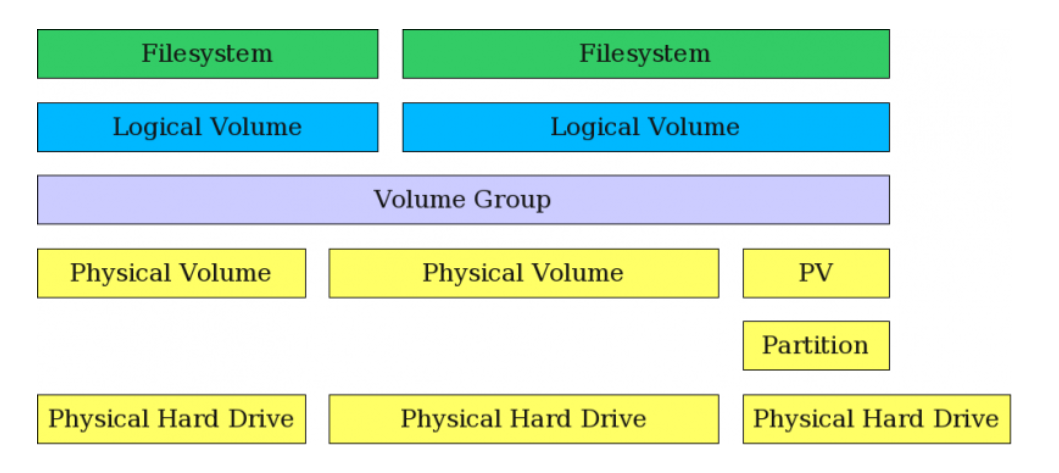
\includegraphics[width=\textwidth]{pictures/pvs.png}
    \centering
\end{figure}

\begin{itemize}
    \item \textbf{Physical Volumes (PV's):} basic storage devices that LVM manages. They can be an entire hard drive, a partition on a hard drive, or a RAID array. PVs are initialized for use by LVM using the \verb|pvcreate| command, which writes metadata to the physical volume so that it can be used by LVM.
    \item \textbf{Volume Groups (VG's):} pool of storage that consists of one or more physical volumes. When you create a VG, you aggregate the storage capacity of all included PVs, making it available for creating logical volumes. The VG acts as a container for logical volumes.
    \item \textbf{Logical Volumes (LV's):} virtual block device that can be used like a regular partition. LVs are created from the storage pool provided by a volume group. You can create, resize, and manage logical volumes without worrying about the underlying physical storage details.
    \item \textbf{Filesystems:} Once a logical volume is created, it must be formatted with a filesystem before it can be used to store files. After formatting, the filesystem can be mounted to a directory in the operating system, making it accessible for reading and writing data.
\end{itemize}

\subsection{Tools to Manage Secondary Storage}

\subsubsection{Lsblk - List block devices}
\textbf{lsblk} is a command-line utility in Linux used to list information about all available or the specified block devices. It shows details about block devices (like hard drives), their partitions, and other types of storage volumes.

\verb|lsblk:| will list all block devices in a tree format showing the hierarchy of devices and their partitions.

\begin{itemize}
    \item \verb|-a| (\verb|--all|): Show all devices, including empty ones.
    \item \verb|-d| (\verb|--nodeps|): Don't print device holders or slaves.
    \item \verb|-f| (\verb|--fs|): Output information about filesystems.
    \item \verb|-o| (\verb|--output|): Define which columns to output.
    \item \verb|-l| (\verb|--list|): Use list format instead of tree format.
    \item \verb|-p| (\verb|--paths|): Print full device paths.
    \item \verb|-r| (\verb|--raw|): Use the raw output format.
    \item \verb|-t| (\verb|--topology|): Show topology information.
    \item \verb|-J| (\verb|--json|): Use JSON output format.
\end{itemize}

\begin{figure}[H]
    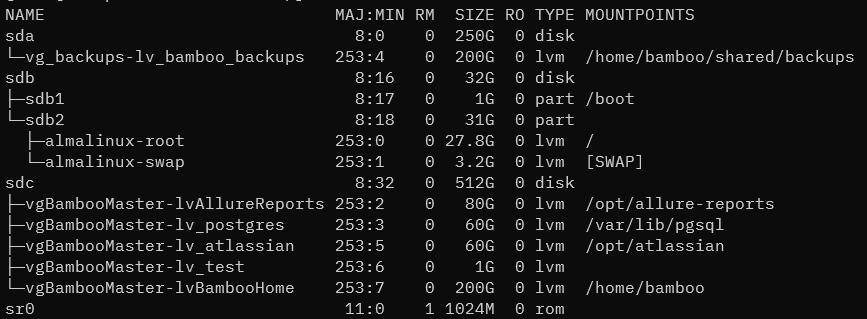
\includegraphics[width=\textwidth]{pictures/lsblk.png}
    \centering
\end{figure}

\begin{figure}[H]
    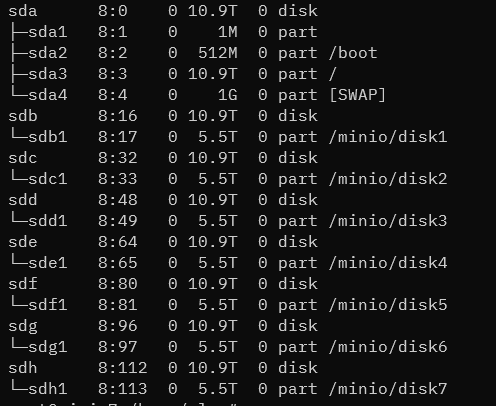
\includegraphics[scale=0.7]{pictures/lsblkm.png}
    \centering
\end{figure}

\subsubsection{Fdisk - Managing Partitions}
\textbf{fdisk} is a command-line utility in Linux used for disk partitioning. It's a powerful tool that allows users to create, delete, resize, and manage disk partitions on hard drives.

\textbf{fdisk} stands for "Fixed Disk" and is primarily used to manipulate partition tables on hard drives. It supports various partition table formats, with the most common being the Master Boot Record (MBR) and GUID Partition Table (GPT).

\verb|fdisk -l:| lists the partition tables of all disk drives, showing the details of each disk and its partitions and volumes:
\begin{itemize}
    \item Disk size
    \item Sector size
    \item Partition type
    \item Partition size
\end{itemize}

\verb|fdisk -l /dev/sdx:| Show the partition table with details of a specific disk.

\textbf{Interactive mode:} \verb|fdisk /dev/sda|
\begin{itemize}
    \item \verb|m|: display the help menu.
    \item \verb|p|: print the partition table.
    \item \verb|n|: add a new partition.
    \item \verb|d|: delete an existing partition.
    \item \verb|t|: change a partition type.
    \item \verb|w|: write the changes into the disk and exit.
    \item \verb|q|: quit without saving changes.
\end{itemize}

\begin{blocktemplateIII}{Warning}
\verb|g| inside \textbf{fdisk} will erase any existing partition table and data on the disk. So it prepares the disk to be partitiones by creating a new a new empty GPT (GUID Partition Table) partition table. 
\end{blocktemplateIII}

\underline{Usage Example:} Iinstall a new partition on drive \verb|/dev/sda| of 5.47TiB:

\begin{enumerate}
    \item Become sudo: \verb|sudo su|
    \item List system disks information: \verb|lsblk|
    \item Start interactive disk \verb|/dev/sda| modification: \verb|fdisk /dev/sda|
\begin{figure}[H]
    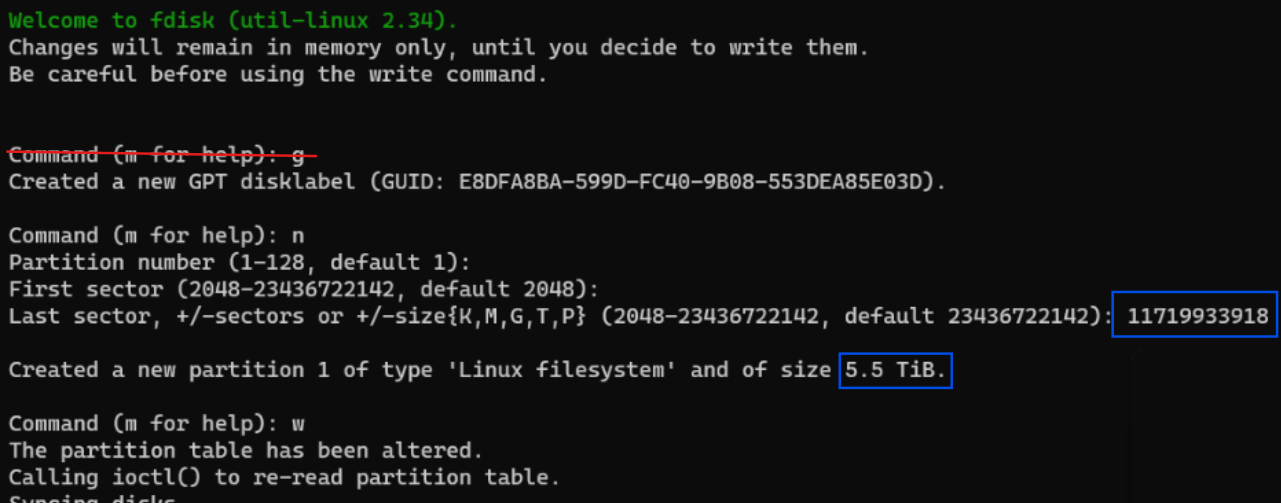
\includegraphics[width=\textwidth]{pictures/fdiskk.png}
    \centering
\end{figure}

    \item Write the changes: \verb|w|
    \item Check the partition has been created: \verb|lsblk| or \verb|fdisk -l /dev/sda|
    \item Format the partition with a filesystem: \verb|mkfs.ext4 /dev/sda1|
    \item Mount the filesystem to a directory in order can be used: \verb|mount /dev/sda1 /mnt/mydata|
    \item Check the filesystems: \verb|df -h|
\end{enumerate}

\subsubsection{LVM - Managing Volumes on Linux}

\paragraph{For PVs}

Displays information about all physical volumes (PVs):
\begin{codetemplate}
\begin{verbatim}
pvdisplay
\end{verbatim}
\end{codetemplate}

Show detailed information about a physical volume:
\begin{codetemplate}
\begin{verbatim}
pvdisplay [options] [PhysicalVolumePath]
\end{verbatim}
\end{codetemplate}

Initialize a partition or drive as a physical volume, making it ready to be used in a volume group:
\begin{codetemplate}
\begin{verbatim}
pvcreate /dev/sda
\end{verbatim}
\end{codetemplate}
\begin{codetemplate}
\begin{verbatim}
pvcreate /dev/sda
\end{verbatim}
\end{codetemplate}

\paragraph{For VGs}

Displays information about volume groups. It shows detailed information such as:
\begin{itemize}
    \item Volume group name
    \item Volume group Size
    \item Free space in the volume group
    \item Number of physical volumes (PVs) in the volume group
    \item Number of logical volumes (LVs) in the volume group
\end{itemize}
\begin{codetemplate}
\begin{verbatim}
vgdisplay
\end{verbatim}
\end{codetemplate}

Displays information about volume groups in a brief format:
\begin{codetemplate}
\begin{verbatim}
vgs
\end{verbatim}
\end{codetemplate}

Displays information about a volume groups:
\begin{codetemplate}
\begin{verbatim}
vgdisplay <vg_name>
\end{verbatim}
\end{codetemplate}

Create a new volume group by combining one or more physical volumes:
\begin{codetemplate}
\begin{verbatim}
vgcreate <vg_name> <pv_name1> <pv_name2> ... <pv_namen>
\end{verbatim}
\end{codetemplate}

Adds one or more physical volumes to an existing volume group:
\begin{codetemplate}
\begin{verbatim}
vgextend <vg_name> <pv_name>
\end{verbatim}
\end{codetemplate}

Removes one or more physical volumes from a volume group:
\begin{codetemplate}
\begin{verbatim}
vgreduce <vg_name> <pv_name>
\end{verbatim}
\end{codetemplate}
    
Removes a volume group from the system: 
\begin{codetemplate}
\begin{verbatim}
vgremove <vg_name>
\end{verbatim}
\end{codetemplate}

\begin{blocktemplateIII}{Warning}
The volume group must be empty (all logical volumes must be removed first).
\end{blocktemplateIII}

Renames an existing volume group:
\begin{codetemplate}
\begin{verbatim}
vgrename old_volume_group new_volume_group
\end{verbatim}
\end{codetemplate}

Scans all disks for volume groups and rebuilds the LVM cache:
\begin{codetemplate}
\begin{verbatim}
vgscan
\end{verbatim}
\end{codetemplate}

Checks the consistency of volume group metadata:
\begin{codetemplate}
\begin{verbatim}
vgck <vg_name>
\end{verbatim}
\end{codetemplate}

\paragraph{For LVs}

Display information about logical volumes. It shows details such as:
\begin{itemize}
    \item Logical volume name
    \item Volume group name
    \item Size of the logical volume
    \item Attributes and status of the logical volume
\end{itemize}
\begin{codetemplate}
\begin{verbatim}
lvdisplay
\end{verbatim}
\end{codetemplate}

Display information about a LV:
\begin{codetemplate}
\begin{verbatim}
lvdisplay /dev/my_volume_group/my_logical_volume
\end{verbatim}
\end{codetemplate}

Display information about logical volumes in a brief format:
\begin{codetemplate}
\begin{verbatim}
lvs
\end{verbatim}
\end{codetemplate}

Create a new logical volume within a specified volume group:
\begin{codetemplate}
\begin{verbatim}
lvcreate -L 10G -n my_logical_volume my_volume_group
\end{verbatim}
\end{codetemplate}

To extend the size of a lv:
\begin{codetemplate}
\begin{verbatim}
lvextend -L +5G /dev/my_volume_group/my_logical_volume
\end{verbatim}
\end{codetemplate}

To reduce the size of a lv:
\begin{codetemplate}
\begin{verbatim}
lvreduce -L -5G /dev/my_volume_group/my_logical_volume
\end{verbatim}
\end{codetemplate}

Resizes a logical volume, either increasing or decreasing its size. This combines lvextend and lvreduce:
\begin{codetemplate}
\begin{verbatim}
lvresize -L +15G /dev/my_volume_group/my_logical_volume
\end{verbatim}
\end{codetemplate}
\begin{codetemplate}
\begin{verbatim}
lvresize -L -15G /dev/my_volume_group/my_logical_volume
\end{verbatim}
\end{codetemplate}

To remove a logical volume:
\begin{codetemplate}
\begin{verbatim}
lvremove /dev/my_volume_group/my_logical_volume
\end{verbatim}
\end{codetemplate}

To rename a logical volume:
\begin{codetemplate}
\begin{verbatim}
lvrename /dev/my_volume_group/my_logical_volume
\end{verbatim}
\end{codetemplate}

Scan all logical volumes in the system and rebuilds the LVM cache:
\begin{codetemplate}
\begin{verbatim}
lvscan
\end{verbatim}
\end{codetemplate}

Change the attributes of a logical volume, such as making it active or inactive.:
\begin{codetemplate}
\begin{verbatim}
lvchange -a y /dev/my_volume_group/my_logical_volume
\end{verbatim}
\end{codetemplate}

\subsubsection{Filesystem}
Report the amount of disk space used and available on filesystems:
\begin{codetemplate}
\begin{verbatim}
df -h
\end{verbatim}
\end{codetemplate}

\begin{itemize}
    \item \verb|-h|: output human-readable by showing sizes in KB, MB, GB, etc.
\end{itemize}

Estimates file space usage:
\begin{codetemplate}
\begin{verbatim}
du -h
\end{verbatim}
\end{codetemplate}

Create a filesystem on a storage device (e.g., a partition or a logical volume) specifying the type of filesystem:
\begin{codetemplate}
\begin{verbatim}
mkfs -t ext4 /dev/sdX1
\end{verbatim}
\end{codetemplate}

Attach a filesystem to the filesystem hierarchy at a specified mount point:
\begin{codetemplate}
\begin{verbatim}
mount /dev/sdxi /path/to/my_mount_point
\end{verbatim}
\end{codetemplate}

\begin{codetemplate}
\begin{verbatim}
mount /dev/vgName/lvName /path/to/my_mount_point
\end{verbatim}
\end{codetemplate}

Detach a filesystem from the filesystem hierarchy.

\begin{codetemplate}
\begin{verbatim}
umount /path/to/my_mount_point
\end{verbatim}
\end{codetemplate}

\textbf{/etc/fstab} file contains a list of entries that define how disk partitions, filesystems, and other block devices should be automatically mounted at boot time.

Example entry in \verb|/etc/fstab| file:
\begin{codetemplate}{/etc/fstab}
\begin{verbatim}
# <file system> <mount point> <type> <options> <dump> <pass>
/dev/vgName/lvName /path/to/my_mount_point ext4 defaults 0 2
\end{verbatim}
\end{codetemplate}

\begin{itemize}
    \item \textbf{Dump}
    \begin{itemize}
        \item 0: The filesystem will not be backed up by the dump command.
        \item 1: The filesystem will be backed up by the dump command.
    \end{itemize}
    \item \textbf{Pass:} which filesystems should be checked at boot time.
    \begin{itemize}
        \item 0: The filesystem will not be checked.
        \item 1: The filesystem will be checked first. This should be used for the root filesystem (/).
        \item 2: The filesystem will be checked after the filesystems with a pass value of 1. This is typically used for all other filesystems.
    \end{itemize}
\end{itemize}

To mount all filesystems specified in verb|/etc/fstab| without rebooting:
\begin{codetemplate}
\begin{verbatim}
mount -a
\end{verbatim}
\end{codetemplate}



\newpage
%-------------------------------------------------------------------------------------------------
\section{Others}

\subsection{Docker Desktop}

\begin{itemize}
    \item Docker desktop corre en nuestro Ubuntu desde Windows. Por tanto, si queremos que el Docker de nuestro Ubuntu tenga los certificados necesarios para conectarse a los recursos de nuestra empresa, debemos tener los certificados descargados, actualizados e instalados en nuestro sistema Windows nativo.
    \item Desde un terminal rellenamos el contenido del fichero de configuración de docker \verb|~/.docker/config.json|:
\begin{codetemplate}{\~/.docker/config.json}
\begin{verbatim}
{
  "auths": {
    "docker-registry.cloud.yourcompany.com": {}
  },
  "credsStore": "desktop.exe",
  "proxies": {
    "default": {
      "httpProxy": "http://urltoproxy",
      "httpsProxy": "http://urltoproxy/"
    }
  }
}
\end{verbatim}
\end{codetemplate}

    \item En Docker Engine modificar el fichero que ahí introducimos por el siguiente:
\begin{codetemplate}{}
\begin{verbatim}
{
  "builder": {
    "gc": {
      "defaultKeepStorage": "20GB",
      "enabled": true
    }
  },
  "experimental": false,
  "features": {
    "buildkit": false
  },
  "insecure-registries": [
    "docker-registry.cloud.yourcompany.com"
  ]
}
\end{verbatim}
\end{codetemplate}

    \item Ejecutar el comando para logearnos contra el registry que hayamos escogido:
\begin{codetemplate}{}
\begin{verbatim}
$ docker login -u USER -p PASSWORD docker-registry.cloud.yourcompany.com
\end{verbatim}
\end{codetemplate}

    \item Probar el acceso al registry:
\begin{codetemplate}{}
\begin{verbatim}
$ docker pull docker-registry.cloud.yourcompany.com/catalog/paas/j
\end{verbatim}
\end{codetemplate} 
\end{itemize}

\subsection{Helm}
\textbf{Compilar}
\newline Estando en el directorio que contiene el fichero Chart.yaml:
\begin{codetemplate}{}
\begin{verbatim}
$ helm lint .
\end{verbatim}
\end{codetemplate}

\textbf{Prueba de despliegue Resources en Cluster with file}
\begin{codetemplate}{}
\begin{verbatim}
$ helm install -f ./values_ssp.yaml . --debug \
--name-template standalone-11 --dry-run > output.yaml
\end{verbatim}
\end{codetemplate}

\textbf{Prueba de despliegue Resources en Cluster with file}
\begin{codetemplate}{}
\begin{verbatim}
$ helm install -f ./values_ssp.yaml . --debug \
--name-template standalone-11
\end{verbatim}
\end{codetemplate}

\subsection{JSONPath}
JSONPath is a query language for JSON, similar to XPath for XML. AlertSite API endpoint monitors let you use JSONPath in assertions to specify the JSON fields that need to be verified.

\subsubsection{Basic Usage}
A JSONPath expression specifies a path to an element (or a set of elements) in a JSON structure. \\ \\
\textbf{Dot Notation}
\begin{codetemplate}{}
\begin{verbatim}
$.store.book[0].title
\end{verbatim}
\end{codetemplate}

\textbf{Bracket Notation}
\begin{codetemplate}{}
\begin{verbatim}
$["store"]["book"][0]["title"]
\end{verbatim}
\end{codetemplate}

\textbf{Mix}
\begin{codetemplate}{}
\begin{verbatim}
["store"].book[0].title
\end{verbatim}
\end{codetemplate}

\begin{blocktemplate}{Nota}
Note that dots are only used before property names not in brackets.
\end{blocktemplate}

\begin{blocktemplateII}{Nota 2}
The leading "\textbf{\textit{\$}}" represents the root object or array and can be omitted. For example, \textbf{\textit{\$.foo.bar}} and \textbf{\textit{foo.bar}} are the same, and so are \textbf{\textit{\$[0].status}} and \textbf{\textit{[0].status}}.
\end{blocktemplateII}

\begin{blocktemplateIII}{Nota 3}
Using Bracket Notation be care to put \textbf{single quotes}, because double quotes are not accepted:
\begin{verbatim}
["name"]
\end{verbatim}
\end{blocktemplateIII}

\begin{blocktemplateIII}{Nota 4}
JSONPath expressions, including property names and values, are case-sensitive.
\end{blocktemplateIII}

\textbf{Syntax Elements}
\begin{itemize}
    \item \verb|$|: The root object or array.
    \item \verb|.property = ["property"]|: Selects the specified property in a parent object.
    \item \verb|[n]|: Select the n-th element from an array. Indexes are 0-based.
    \item \verb|[index1,index2,…]|: Selects array elements with the specified indexes. Returns a list.
    \item \verb|..property|: Recursive descent: Searches for the specified property name recursively and returns an array of all values with this property name. Always returns a list, even if just one property is found.
    \item \verb|*|: Wildcard selects all elements in an object or an array, regardless of their names or indexes. For example, address. "*" means all properties of the address object, and book[*] means all items of the book array.
    \item \verb|[:n]|: Selects the first n elements of the array. Returns a list.
    \item \verb|[-n]|: Selects the last n elements of the array. Returns a list.
\end{itemize}

\subsubsection{Filters}
We can use some expression to filter the output of the JSON in function of parameters introduced in the syntax.
\\
\\
\textbf{Syntax Elements}
\begin{itemize}
    \item \verb|[?(expression)]|: Filter expression. Selects all elements in an object or array that match the specified filter. Returns a list.
    \item \verb|@|: Used in filter expressions to refer to the current node being processed.
\end{itemize}

\subsubsection{Example}
\begin{codetemplate}{JSON Example}
\begin{verbatim}
{
  "store": {
    "book": [
      {
        "category": "reference",
        "author": "Nigel Rees",
        "title": "Sayings of the Century",
        "price": 8.95
      },
      {
        "category": "fiction",
        "author": "Herman Melville",
        "title": "Moby Dick",
        "isbn": "0-553-21311-3",
        "price": 8.99
      },
      {
        "category": "fiction",
        "author": "J.R.R. Tolkien",
        "title": "The Lord of the Rings",
        "isbn": "0-395-19395-8",
        "price": 22.99
      }
    ],
    "bicycle": {
      "color": "red",
      "price": 19.95
    }
  },
  "expensive": 10
}
\end{verbatim}
\end{codetemplate}

\underline{Expressions}

\begin{blocktemplate}{Nota}
In all these examples, the leading \$. is optional and can be omitted.
\end{blocktemplate}

\begin{codetemplate}{}
\begin{verbatim}
$.store.* = ["store"][*]
\end{verbatim}
\end{codetemplate}
\begin{itemize}
    \item \textbf{Meaning:} All direct properties of store (not recursive).
    \item \textbf{Result:}
\begin{verbatim}
[
    "book": [
        {
            "category": "reference",
            "author": "Nigel Rees",
            "title": "Sayings of the Century",
            ...
        },
        { ...
        }
    ],
    "bicycle": {
        "color": "red",
        ...
    }
]
\end{verbatim}
\end{itemize}

\begin{codetemplate}{}
\begin{verbatim}
$.store.bicycle.color = ["store"]["bicycle"]["color"]
\end{verbatim}
\end{codetemplate}
\begin{itemize}
    \item \textbf{Meaning:} The color of the bicycle in the store.
    \item \textbf{Result:} \verb|red|
\end{itemize}

\begin{codetemplate}{}
\begin{verbatim}
$.store..price = \$..price = ..["price"]
\end{verbatim}
\end{codetemplate}
\begin{itemize}
    \item \textbf{Meaning:} The prices of all items in the store.
    \item \textbf{Result:} \verb+[8.95, 8.99, 22.99, 19.95]+
\end{itemize}

\begin{codetemplate}{}
\begin{verbatim}
$.store.book[*] = \$..book[*] = ..["book"][*]
\end{verbatim}
\end{codetemplate}
\begin{itemize}
    \item \textbf{Meaning:} All books in the store.
    \item \textbf{Result:}
\begin{verbatim}
[
  {
    "category":"reference",
    "author":"Nigel Rees",
    "title":"Sayings of the Century",
    "price":8.95
  },
  {
    "category":"fiction",
    "athor":"J.R.R. Tolkien"
    ...
  }
]
\end{verbatim}
\end{itemize}

\begin{codetemplate}{}
\begin{verbatim}
$..book[*].title = ..["book"][*]["title"]
\end{verbatim}
\end{codetemplate}
\begin{itemize}
    \item \textbf{Meaning:} The title of all books in the store.
    \item \textbf{Result:}
\begin{verbatim}
[   
    Sayings of the Century, 
    Moby Dick,
    The Lord of the Rings 
]
\end{verbatim}
\end{itemize}

\begin{codetemplate}{}
\begin{verbatim}
$..book[0]
\end{verbatim}
\end{codetemplate}
\begin{itemize}
    \item \textbf{Meaning:} The first book.
    \item \textbf{Result:}
\begin{verbatim}
[
  {
    "category":"reference",
    "author":"Nigel Rees",
    "title":"Sayings of the Century",
    "price":8.95
  }
]
\end{verbatim}

\end{itemize}

\begin{codetemplate}{}
\begin{verbatim}
$..book[0].title
\end{verbatim}
\end{codetemplate}
\begin{itemize}
    \item \textbf{Meaning:} The title of the first book.
    \item \textbf{Result:} \verb+Sayings of the Century+
\end{itemize}

\begin{codetemplate}{}
\begin{verbatim}
$..book[0,1].title
\end{verbatim}
\end{codetemplate}
\begin{itemize}
    \item \textbf{Meaning:} The titles of the first two books.
    \item \textbf{Result:} \verb+[Sayings of the Century, Moby Dick]+
\end{itemize}

\begin{codetemplate}{}
\begin{verbatim}
$..book[-1:].title
\end{verbatim}
\end{codetemplate}
\begin{itemize}
    \item \textbf{Meaning:} The title of the last book.
    \item \textbf{Result:} \verb+The Lord of the Rings+
\end{itemize}

\begin{codetemplate}{}
\begin{verbatim}
$..book[?(@.author=="J.R.R. Tolkien")].title
\end{verbatim}
\end{codetemplate}
\begin{itemize}
    \item \textbf{Meaning:} The titles of all books by J.R.R. Tolkien (exact match, case-sensitive).
    \item \textbf{Result:} It is a list because -n always returns a list. \verb|[The Lord of the rings]|
\end{itemize}

\begin{codetemplate}{}
\begin{verbatim}
$..book[?(@.isbn)]
\end{verbatim}
\end{codetemplate}
\begin{itemize}
    \item \textbf{Meaning:} All books that have the isbn property.
    \item \textbf{Result:} \verb+[Moby Dick, The Lord of the Rings]+
\end{itemize}

\begin{codetemplate}{}
\begin{verbatim}
$..book[?(!@.isbn)]
\end{verbatim}
\end{codetemplate}
\begin{itemize}
    \item \textbf{Meaning:} All books without the isbn property.
    \item \textbf{Result:} \verb+[Saying of the Century]+
\end{itemize}

\begin{codetemplate}{}
\begin{verbatim}
$..book[?(@.price < 10)].title
\end{verbatim}
\end{codetemplate}
\begin{itemize}
    \item \textbf{Meaning:} All books cheaper than 10 titles.
    \item \textbf{Result:} \verb+[Sayings of the Century, Moby Dick]+
\end{itemize}

\begin{codetemplate}{}
\begin{verbatim}
$..book[?(@.price > \$.expensive)]
\end{verbatim}
\end{codetemplate}
\begin{itemize}
    \item \textbf{Meaning:} All expensive books.
    \item \textbf{Result:} 
\begin{verbatim}
$ [
    {
      "category": "fiction",
      "author": "J.R.R. Tolkien",
      "title": "The Lord of the Rings",
      "isbn": "0-395-19395-8",
      "price": 22.99
    }
  ]
\end{verbatim}
\end{itemize}

\begin{codetemplate}{}
\begin{verbatim}
$..book[?(@.category == "fiction" ||
@.category == "reference")].title
\end{verbatim}
\end{codetemplate}
\begin{itemize}
    \item \textbf{Meaning:} All fiction and reference books titles.
    \item \textbf{Result:} \verb|[Sayings of the Century, Moby Dick, The Lord of The Rings]|
\end{itemize}

\begin{codetemplate}{}
\begin{verbatim}
$..book[?(@.category != "fiction")]
\end{verbatim}
\end{codetemplate}
\begin{itemize}
    \item \textbf{Meaning:} All not fiction books.
    \item \textbf{Result:}
\end{itemize}
\begin{verbatim}
[
  {
    "category":"reference",
    "author":"Nigel Rees",
    "title":"Sayings of the Century",
    "price":8.95
  }
]
\end{verbatim}

For more information about JSONPath, check the following \href{https://support.smartbear.com/alertsite/docs/monitors/api/endpoint/jsonpath.html}{page}

\subsubsection{JSONPath K8s} \label{jsonpath k8s}
JSONPath template is composed of JSONPath expressions enclosed by curly braces {}. Kubectl uses JSONPath expressions to filter on specific fields in the JSON object and format the output. In addition to the original JSONPath template syntax, the following functions and syntax are valid:
\begin{itemize}
    \item \verb|range, end|: iterate list. \verb|{range .items[*]}{.metadata.name}|
    \item \verb|{"\n}, {"\t"}|: to write salto de linea or tab. \verb|{..metadata.name}{"\t"}{..matadata.image}|
\end{itemize}

\underline{Example 1} 
\\
\\
Get all \textbf{containers} / \textbf{initContainers} running and their images used inside a \textbf{Pod} or declared in pod.spec of \textbf{ Deployment/Statefulset} . It is exactly the same changing little things. At least, it is showed in column view separed by tab.
\begin{codetemplate}{}
\begin{verbatim}
$ kc get RESOURCE_TYPE RESOURCE_NAME \
-o jsonpath="{range ..containers[*]}{.name}{"\t"}{.image}{"\n"}" \
|sort|column -t
\end{verbatim}
\end{codetemplate}
\begin{enumerate}
    \item To choose between \textbf{Pod} or \textbf{Deploy/Sateful}: modify  \verb|RESOURCE_TYPE & RESOURCE_NAME|
    \item To choose between \textbf{containers} or \textbf{initContainers}: modify the range.
    \begin{itemize}
        \item containers:  \verb|{range ..containers[*]}|
        \item initContainers: \verb|{range ..initContainers[*]}|
    \end{itemize}
\end{enumerate}

\begin{figure}[H]
    \centering
    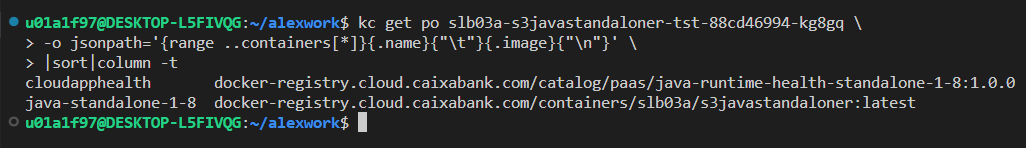
\includegraphics[scale=0.5]{pictures/image18.png}
    \caption{Get all containers parsing a Pod JSON}
    \label{parsing json 1}
\end{figure}
\begin{figure}[H]
    \centering
    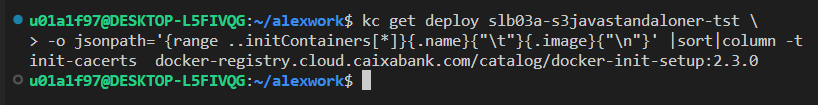
\includegraphics[scale=0.54]{pictures/image19.png}
    \caption{Get all initContainers parsing a Deployment JSON}
    \label{parsing json 2}
\end{figure}

\underline{Example 2} 
\\
\\
Get all ports exposed by a Pod, Deployment or Statefulset.
\begin{codetemplate}{}
\begin{verbatim}
$ kc get RESOURCE_TYPE RESOURCE_NAME \ 
-o jsonpath="{range ..containers[*]}{.name}{"\t"}{.ports}{"\n"}" \ 
|sort|column -t
\end{verbatim}
\end{codetemplate}
\begin{figure}[H]
    \centering
    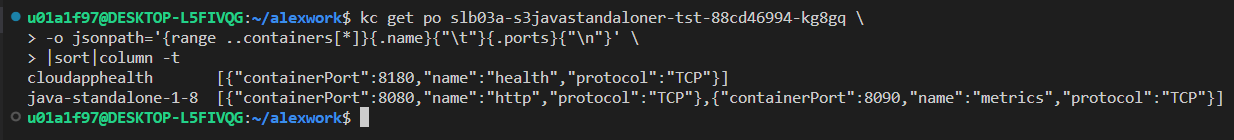
\includegraphics[scale=0.4]{pictures/image20.png}
    \caption{Get all ports exposed in a Pod parsing a Pod JSON}
    \label{parsing json 3}
\end{figure}
\begin{figure}[H]
    \centering
    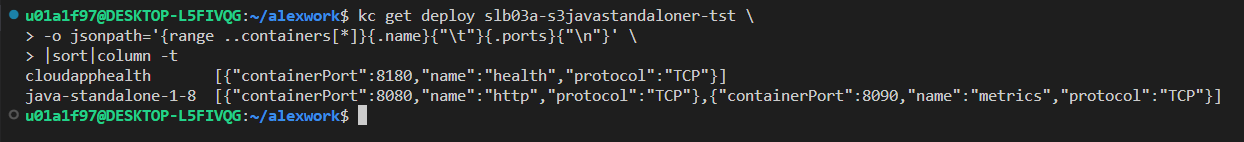
\includegraphics[scale=0.4]{pictures/image21.png}
    \caption{Get all ports exposed in a Pod parsing a Deployment JSON}
    \label{parsing json 4}
\end{figure}

\underline{Example 3} 
\\
\\
Get all Volume Mounts of container called \verb|CONTAINER_NAME| inside a Pod, Deployment or Statefulset.
\begin{codetemplate}{}
\begin{verbatim}
$  kc get RESOURCE_NAME -o jsonpath=\
"{range ..containers[?(@.name == "CONTAINER_NAME")]\
.volumeMounts[*]}.{.name}{"\t"}{.mountPath}{"\n"}" \
|sort|column -t
\end{verbatim}
\end{codetemplate}

\begin{figure}[H]
    \centering
    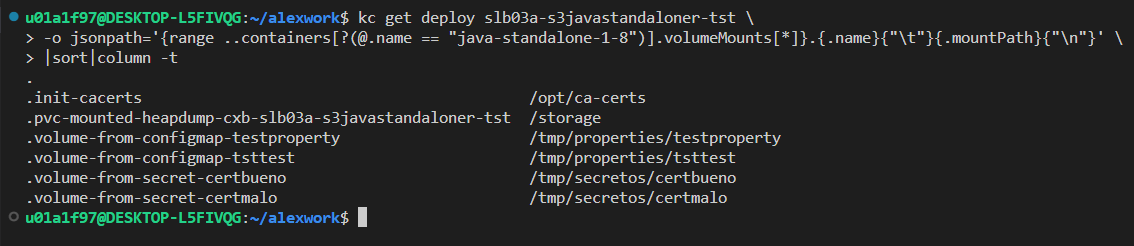
\includegraphics[scale=0.35]{pictures/image23.png}
    \caption{Get all volumeMounts in a container parsing a Deployment JSON}
    \label{parsing json 5}
\end{figure}

\subsection{Ubuntu vs RH7}
Ubuntu es una distribución de Linux que se basa en un kernel Debian, lo que significa que no funciona exactamente igual que otras distribuciones con otros kernel. RH7 al igual que Centos (Open Source) trabajan con un kernel diferente y por tanto los comandos son diferentes. Por ejemplo el gestor de paquetes de Debian es apt-get y el de RH7 es yum.

\subsection{Vagrant}
Vagrant is a tool for building and managing virtual machine environments in a single workflow.

\begin{itemize}
    \item \textbf{vagrant global-status:} nos muestra el estado de todas las maquinas vagrant que tenemos corriendo. Ojo! \textcolor{red}{This data is cached and may not be completely up-to-date (use "vagrant global-status \texttt{--}prune" to prune invalid entries)}.
    \item \textbf{vagrant global-status \texttt{--}prune:} same as before, but up-to-date.
   \item \textbf{vagrant status vagrant\_id or vagrant\_name:} shows the status of the vagrant with "vagrant\_id" or "vagrant\_name" (vagrant\_name == cloudlabxxx)
   \item \textbf{vagrant up vagrant\_name:} initialize a new vagrant with the id "vagrant\_id", it can take a lot of time (15 minutes).
   \item \textbf{vagrant halt vagrant\_id or vagrant\_name:} stops the vagrant
   \item \textbf{vagrant destroy -f vagrant\_id or vagrant\_name:} destroy the vagrant with the id "vagrant\_id", you lose all your configurations, but not your data into /vagrant.
   \item \textbf{ps -ef \texttt{|} grep cloudlabxxx:} show the processes running in vagrant.
   \item \textbf{kill -9 process\_id:} kill the process with "process\_id"
\end{itemize}

\subsection{Red Had Package Installer}
\subsubsection{RPM}
\textbf{RPM (Red Hat Package Manager)} is a free open and \textbf{powerful package management system}. The name refers to file format \textbf{.rpm} and the package manager program itself. An RPM package can contain an arbitrary set of files. Most RPM files are “binary RPMs" (or BRPMs) containing the compiled version of some software. There are also “source RPMs" (or SRPMs) containing the source code used to build a binary package.

It is capable of:

\begin{itemize}
    \item \textbf{Building computer software from source} into easily distributable packages.
    \item \textbf{Installing, updating and uninstalling} packaged software.
    \item \textbf{Querying detailed information} about the packaged software, whether installed or not.
    \item \textbf{Verifying integrity} of packaged software and resulting software installation.
\end{itemize}

\subsubsection{YUM}

\subsection{Timeshift to Backup and Restore Your Linux System}

\subsubsection{Introduction}
Linux is susceptible to system failures caused by incorrect commands or system operations. So if you use Linux on your main computer, you may frequently encounter problems. Fortunately, there are system restoration tools that create snapshots of your files and settings, which you can restore on your system to put it back to its previous functioning point in case any of your operations renders it unusable.

Timeshift works by creating a snapshot of your system using either rsync or btrfs mode, depending on your Linux distro. To do this, what Timeshift essentially does is create a restore point for your system at a time when everything's running smoothly. This backup includes all the system files and settings—and no user files or documents. That way, when you accidentally mess up something on your system while configuring or customizing it, you can restore it back to this restore point and revert all your changes.

\subsubsection{Timeshift Installation}
The first step is install timeshift, depending on your system you will use different commands. For Ubuntu:
\begin{codetemplate}{}
\begin{verbatim}
$ sudo apt install timeshift
\end{verbatim}
\end{codetemplate}

\subsubsection{Create a Snapshot}
\begin{codetemplate}{}
\begin{verbatim}
$ sudo timeshift --create --comments "A new backup" --tags D
\end{verbatim}
\end{codetemplate}

\end{document}
